\date{}
\title{}
\date{}
\usepackage{pgfplots}
\pgfplotsset{compat=1.16}
\begin{document}
\begin{frame}
    \titlepage
\end{frame}



\begin{frame}{last time}
    \begin{itemize}
    \item logistics
        \begin{itemize}
        \item homework, quiz
        \end{itemize}
    \item terms
        \begin{itemize}
        \item hosts, nodes, switches, routers, links
        \item flows
        \end{itemize}
    \item different interfaces / stream abstraction
    \item layered design
    \item wireshark
    \end{itemize}
\end{frame}

\begin{frame}{anonymous feedback}
    \begin{itemize}
    \item ``Can the full logistics slides be posted onto the schedule? Minor typo on the canvas homepage; it says "Submussion site" instead of "Submission site"''
    \end{itemize}
\end{frame}

\subsection{OSI/Internet model}

\usetikzlibrary{calc}

\begin{frame}{OSI model}
\begin{tikzpicture}
\node (osi) at (0,0) {
    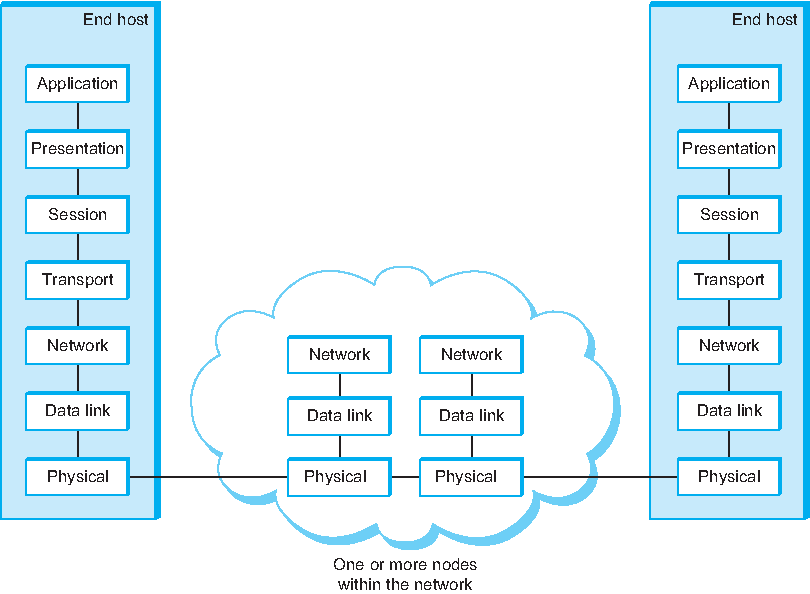
\includegraphics[height=0.75\textheight]{../intro/systemsapproach-1-fig-13.pdf}
};
\coordinate[overlay] (explain loc) at ([yshift=1cm,xshift=0cm]osi.north east);
\tikzset{
    explain box/.style={font=\small,alt=<2>{draw=red}{draw=black},very thick,align=left,at={(explain loc)}, anchor=north west},
    alt explain box/.style={draw=red,ultra thick,anchor=north east,align=left,at={([yshift=-1cm]explain loc)},fill=white},
}
\begin{visibleenv}<2->
\node[overlay,explain box] {
    (7) \myemph<3>{application}: \\ \hspace{.5cm}what requests/etc. \\
    (6) \myemph<3>{presentation}: \\ \hspace{.5cm}data format \\
    (5) \myemph<3>{session}: \\ \hspace{.5cm}manage group of streams \\
    (4) transport: \\ \hspace{.5cm}streams of data \\
    (3) network: \\ \hspace{.5cm}message to correct network \\
    (2) data link: \\ \hspace{.5cm}message $\rightarrow$ bits \\
    \hspace{.5cm}message to correct machine \\
    (1) physical: \\ \hspace{.5cm}send bits/\ldots 
};
\end{visibleenv}
\begin{visibleenv}<3>
\node[overlay,alt explain box] {
    current Internet \\
    usually* layers 5--7 merged together
};
\end{visibleenv}
\end{tikzpicture}
\imagecredit{Figure 13 of Chapter 1 of Computer Networks: A Systems Approach (6th ed) (Peterson and Davie)}
\end{frame}

\begin{frame}<0>{OSI model (text)}
\begin{tabular}{lll} \hline
7 & \myemph<2>{application} & what requests/etc. \\ \hline 
6 & \myemph<2>{presentation} & format of data \\ \hline 
5 & \myemph<2>{session} & coordinate multiple streams \\ \hline
4 & transport & streams of data \\ \hline
3 & network & message to correct network \\ \hline
2 & data link & message to correct machine \\ 
~ & ~ & message into bits/symbols \\
1 & physical & transmit bits/symbols on medium \\
\end{tabular}
\begin{itemize}
\item<2-> \myemph<2>{internet: usually combines layers 7/6/5}
\end{itemize}
\end{frame}

\begin{frame}{OSI model}
    \begin{itemize}
    \item standardized by ISO (International Standards Organization) and ITU (International Telecommunications Union)
    \item full set of protocols\ldots
        \begin{itemize}
        \item file transfer, message sending, directory lookups \ldots
        \end{itemize}
    \item that were often implemented and sometimes used\ldots
    \item but mostly lost out to IETF-standardized Internet protocols
        \begin{itemize}
        \item Internet Engineering Task Force
        \end{itemize}
    \end{itemize}
\end{frame}

\begin{frame}{OSI influence (1)}
    \begin{itemize}
    \item term `layer 7', `layer 4', `layer 3', etc. almost always refer to OSI model
    \item \ldots even though most of Internet does not follow it
        \begin{itemize}
        \item early Internet protocols predate OSI
        \end{itemize}
    \end{itemize}
\end{frame}

\begin{frame}{OSI influence (2)}
    \begin{itemize}
    \item are a lot of Internet protocols influenced by OSI protocols
    \vspace{.5cm}
    \item OSI's DAP (directory access protocol) 
        \begin{itemize}
        \item adapted into IETF's LDAP (lightweight directory access protocol)
        \end{itemize}
    \item OSI presentation layer ASN.1 used in\ldots
        \begin{itemize}
        \item telephony (between telephone companies)
        \item inter-bank messaging
        \item lots of cryptography-related protocols
        \item \ldots
        \end{itemize}
    \item OSI's routing protocol IS-IS still common in large Internet-connected networks
        \begin{itemize}
        \item (adapted to work alongside IETF protocols)
        \end{itemize}
    \end{itemize}
\end{frame}

\begin{frame}{Internet layers}
\small
\begin{tabular}{|l|l|l|p{6cm}|} 
OSI layer & name & examples & purpose \\ \hline
7 & application & HTTP, SSH, & {application-defined meanings}\\
~ & ~ & SMTP, DNS, \ldots & ~ \\ \hline
4 & {transport} & TCP, UDP, \ldots & {reach correct program,\linebreak \myemph<2>{reliablity/streams}} \\ \hline
3 & {network} & IPv4, IPv6, \ldots & {reach correct machine}\linebreak(across networks) \\ \hline
2 & {link} & Ethernet, Wi-Fi, \ldots & {coordinate shared wire/radio}\\ \hline
1 & physical & \ldots & encode bits for wire/radio \\ \hline
\end{tabular}
\end{frame}

\begin{frame}{Internet protocols and layers (non-exhaustive)}
\begin{tikzpicture}
\node[anchor=north west] (int) at (0,0) {
    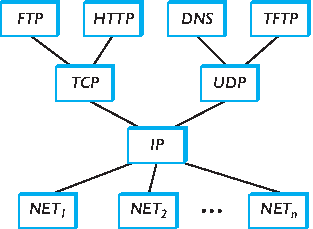
\includegraphics[height=0.75\textheight]{../intro/systemsapproach-1-fig-14.pdf}
};
%\draw[help lines] (0, 0) grid (14, -8);
%\draw[step=2,draw,thick,red] (0, 0) grid (14, -8);
\tikzset{
    layer hi/.style={draw=red,ultra thick},
    layer label/.style={anchor=west},
}
\draw[layer hi] (0, 0) rectangle (9, -1.3);
\node[layer label] at (9.1, -0.65) { application {\it\small OSI layer 7} };
\draw[layer hi] (1.5, -1.8) rectangle (7.5, -3.2);
\node[layer label] at (8.6, -2.5) { transport {\it\small OSI layer 4} };
\draw[layer hi,alt=<2>{fill=red,fill opacity=0.1}] (3.5, -3.6) rectangle (5.6, -4.85);
\node[layer label] at (5.8, -4.2) (net label) { network {\it\small OSI layer 3} };
\draw[layer hi] (0.5, -5.5) rectangle (9, -6.6);
\node[layer label] at (9.1, -6) { data link {\it\small OSI layer 2} };
\begin{visibleenv}<2>
    \node[anchor=west,red,font=\large] at (net label.east) {``narrow waist''};
\end{visibleenv}
\end{tikzpicture}
\imagecredit{Figure 14 of Chapter 1 of Computer Networks: A Systems Approach (6th ed) (Peterson and Davie)}
\end{frame}




\section{interlude: wireshark preview}

% FIXME:
\begin{frame}\frametitle{packet capture tools}
    \begin{itemize}
    \item packet capture = log of everything sent/received on some link(s)
    \item wireshark is popular tool for making, analyzing packet captures
    \vspace{.5cm}
    \item will be showing screenshots from that
    \vspace{.5cm}
    \item you can download these packet captures, follow along in wireshark
    \end{itemize}
\end{frame}

% FIXME: HTTPS

\subsection{some examples in wireshark}
\usetikzlibrary{arrows.meta,decorations.pathreplacing}
\begin{frame}[fragile]{}
\begin{tikzpicture}
\tikzset{
    overlay box/.style={fill=white,fill opacity=0.9}
}
\node[overlay,anchor=north west,inner sep=0mm] (base) at (0, 0) {
    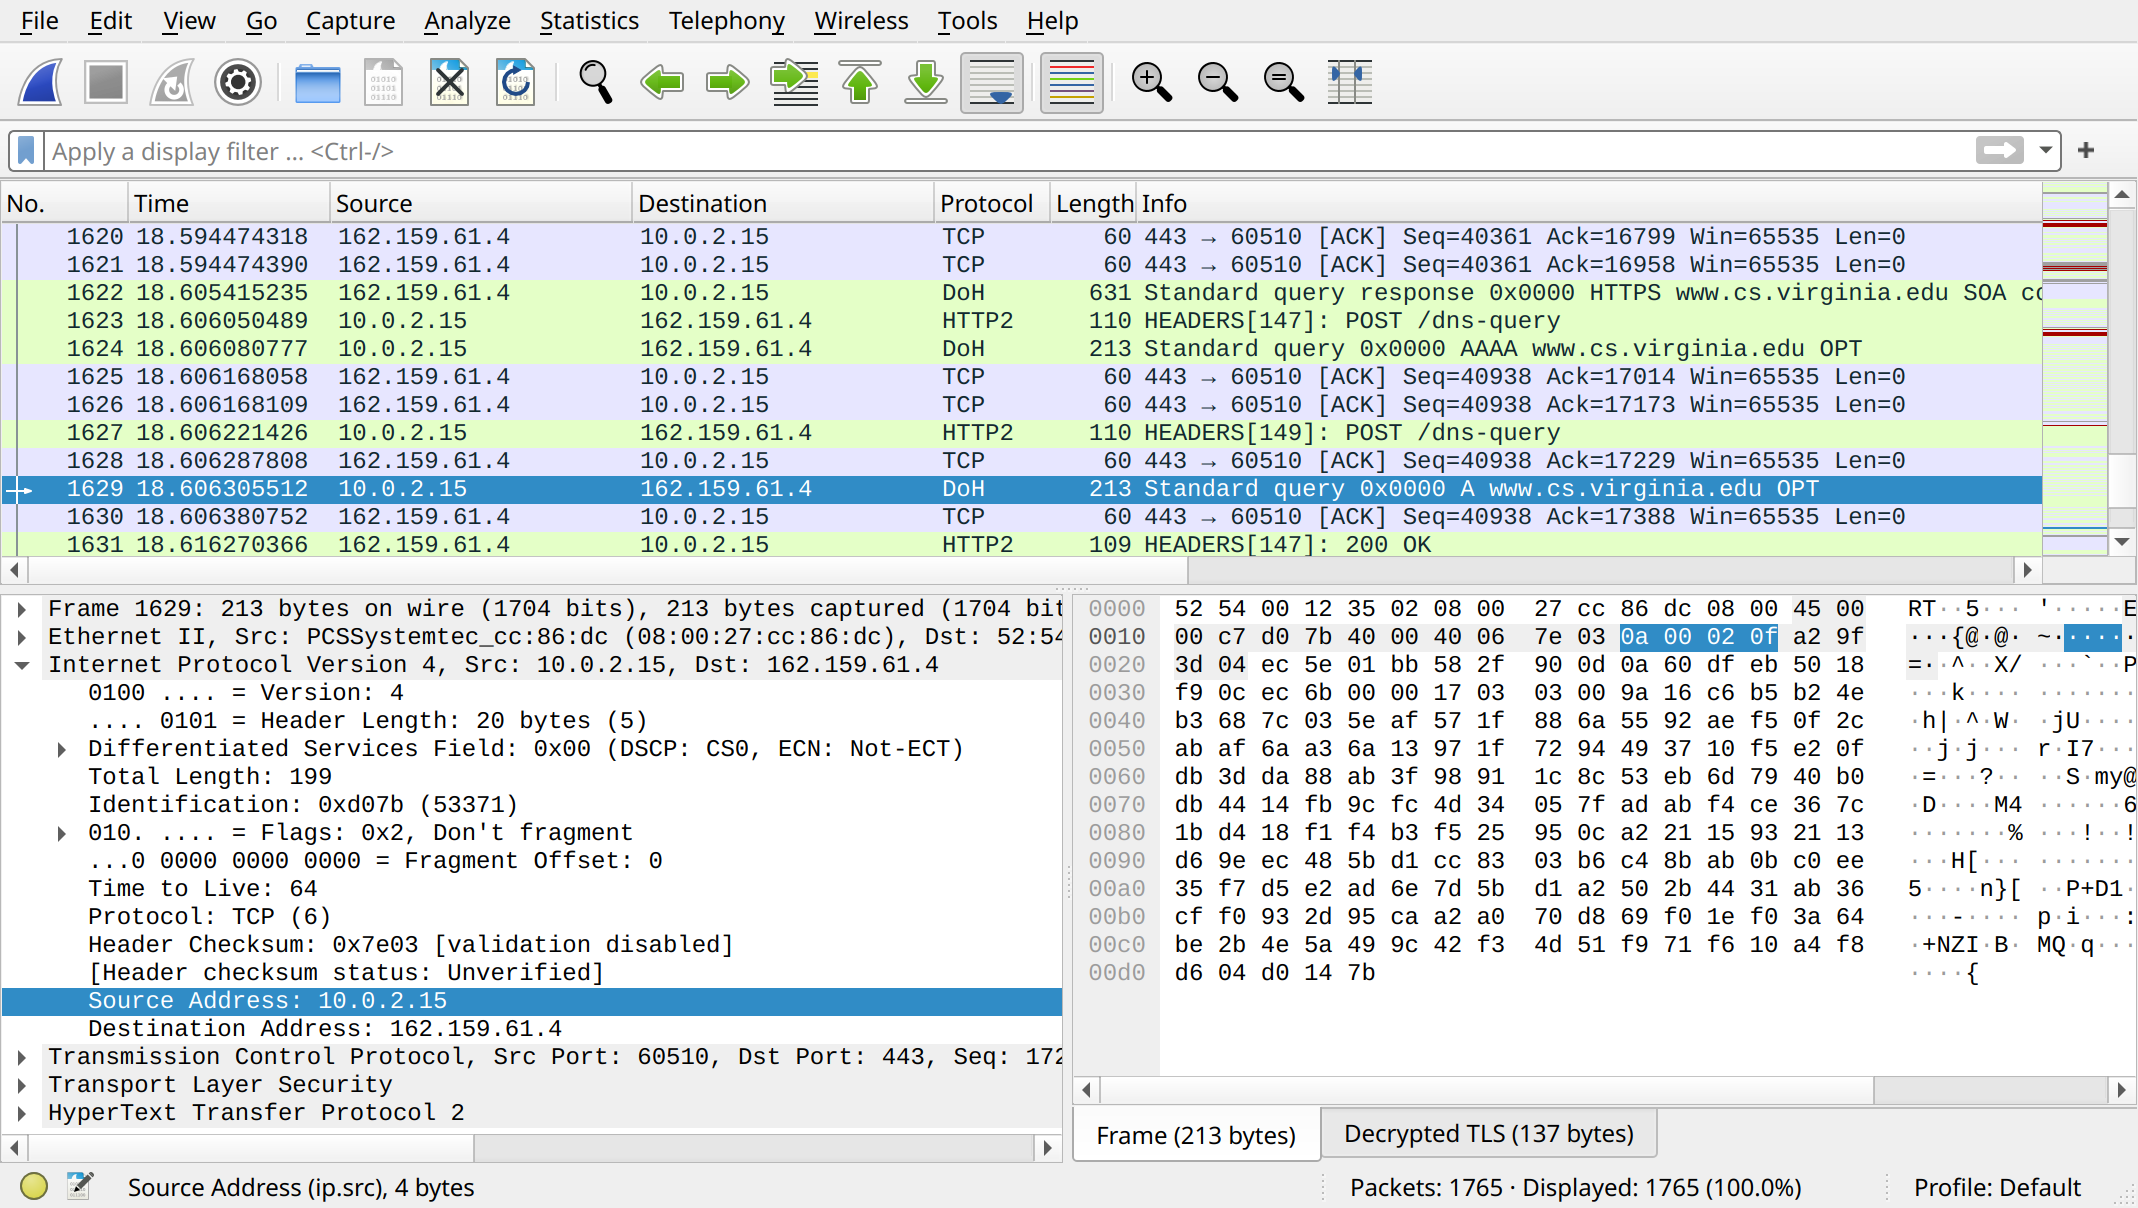
\includegraphics[width=\textwidth]{../intro/wireshark-example1.png}
};
\begin{visibleenv}<1>
    \node[text=red,overlay box] at (7.5, -2) {wireshark window};
\end{visibleenv}
\path (0, 0) rectangle (14.5, -7); % for bounding box
%\draw[overlay,help lines] (0, 0) grid (14, -8);
\begin{visibleenv}<3>
    \path[draw,red,very thick] (0, -1.2) rectangle (14.5, -4)
        node[midway,overlay box] { packet list };
    \path[draw,red,very thick] (0, -4) rectangle (7.25, -7.9)
        node[midway,overlay box] { packet details };
    \path[draw,red,very thick] (7.25, -4) rectangle (14.5, -7.9)
        node[midway,overlay box] { packet bytes };
\end{visibleenv}
\begin{visibleenv}<4>
    \path[draw,red,very thick] (0, -6.7) rectangle (7.2, -6.9);
    \path[draw,red,very thick] (10.93, -4.2) rectangle (12.1, -4.4);
    \path[draw,red,ultra thick] (7.2, -6.8) -- (10.93, -4.3)
        node[midway,above left,overlay box,align=left] {
            hilite in details \\
            shows corresponding bytes
        }
        node[midway,below right,overlay box,font=\fontsize{10}{11}\selectfont,text=black,align=left] {
            this case: \\
            \texttt{10} = \texttt{0x0a} \\
            \texttt{0} = \texttt{0x00} \\
            \texttt{2} = \texttt{0x02} \\
            \texttt{15} = \texttt{0x0f}
        };
\end{visibleenv}
\begin{visibleenv}<5>
    \path[draw,red,very thick] (6.3, -1.2) rectangle (7.15, -4);
    \node[overlay box,anchor=west] at (7.15, -3) (protocol) {`protocol'};
    \node[overlay box,font=\small,anchor=north west] at (protocol.south west) {
        the highest-layer protocol decoded
    };
\end{visibleenv}
\begin{visibleenv}<6-7>
    \begin{scope}
        \begin{pgfinterruptboundingbox}
    \tikzset{invclip/.style={clip,insert path={{[reset cm]
          (-16383.99999pt,-16383.99999pt) rectangle (16383.99999pt,16383.99999pt)
      }}}}
        \path[invclip] (6.3, -3.2) rectangle (7.15, -3.4);
        \end{pgfinterruptboundingbox}

        \fill[overlay,white,fill opacity=0.8] (0, 0) rectangle (14.5, -1.2);
        \fill[white,fill opacity=0.8] (0, -1.2) rectangle (14.5, -4);
        \fill[white,fill opacity=0.8] (7.25, -4) rectangle (14.5, -7.9);
    \end{scope}
    \path[draw,red,very thick] (0, -4) rectangle (7.25, -7.9);
    \tikzset{
        protomark/.style={Latex-,blue,thick},
        protomark brace/.style={blue,thick,decorate,decoration={brace}},
        protomark label/.style={blue,fill=white,fill opacity=0.9},
    }
    \draw[protomark] (7.25, -4.3) -- ++(1, 0) node[right,protomark label] {ethernet};
    \draw[protomark brace] (7.3, -4.5) -- (7.3, -7.1);
        \draw[protomark] (7.4, -5.8) -- ++ (0.75, .6) node[right, protomark label] {
                IPv4 (internet protocol version 4)
        };
    \draw[protomark] (7.25, -7.2) -- ++(1, 1) node[right,protomark label] {
        TCP ({\fontsize{10}{11}\selectfont transmission control protocol})
    };
    \draw[protomark] (7.25, -7.325) -- ++(1, .5) node[right,protomark label] {
        TLS ({\fontsize{10}{11}\selectfont transport layer security})
    };
    \draw[protomark] (7.25, -7.45) -- ++(1, -.2) node[right,protomark label] {
        HTTP/2 ({\fontsize{10}{11}\selectfont hypertext transfer protocol 2})
    };
\end{visibleenv}
\begin{visibleenv}<7>
    \draw[red, very thick] (6.3, -3.2) rectangle (7.15, -3.4);
    \draw[red,Latex-,very thick] (7.15, -3.3) -- ++(1, 0) node[right,align=left,overlay box] {
        DoH is not \\one of these!
    };
\end{visibleenv}
\end{tikzpicture}
\end{frame}

\begin{frame}{}
\begin{tikzpicture}
\tikzset{
    overlay box/.style={fill=white,fill opacity=0.9}
}
\node[overlay,anchor=north west,inner sep=0mm] (base) at (0, 0) {
    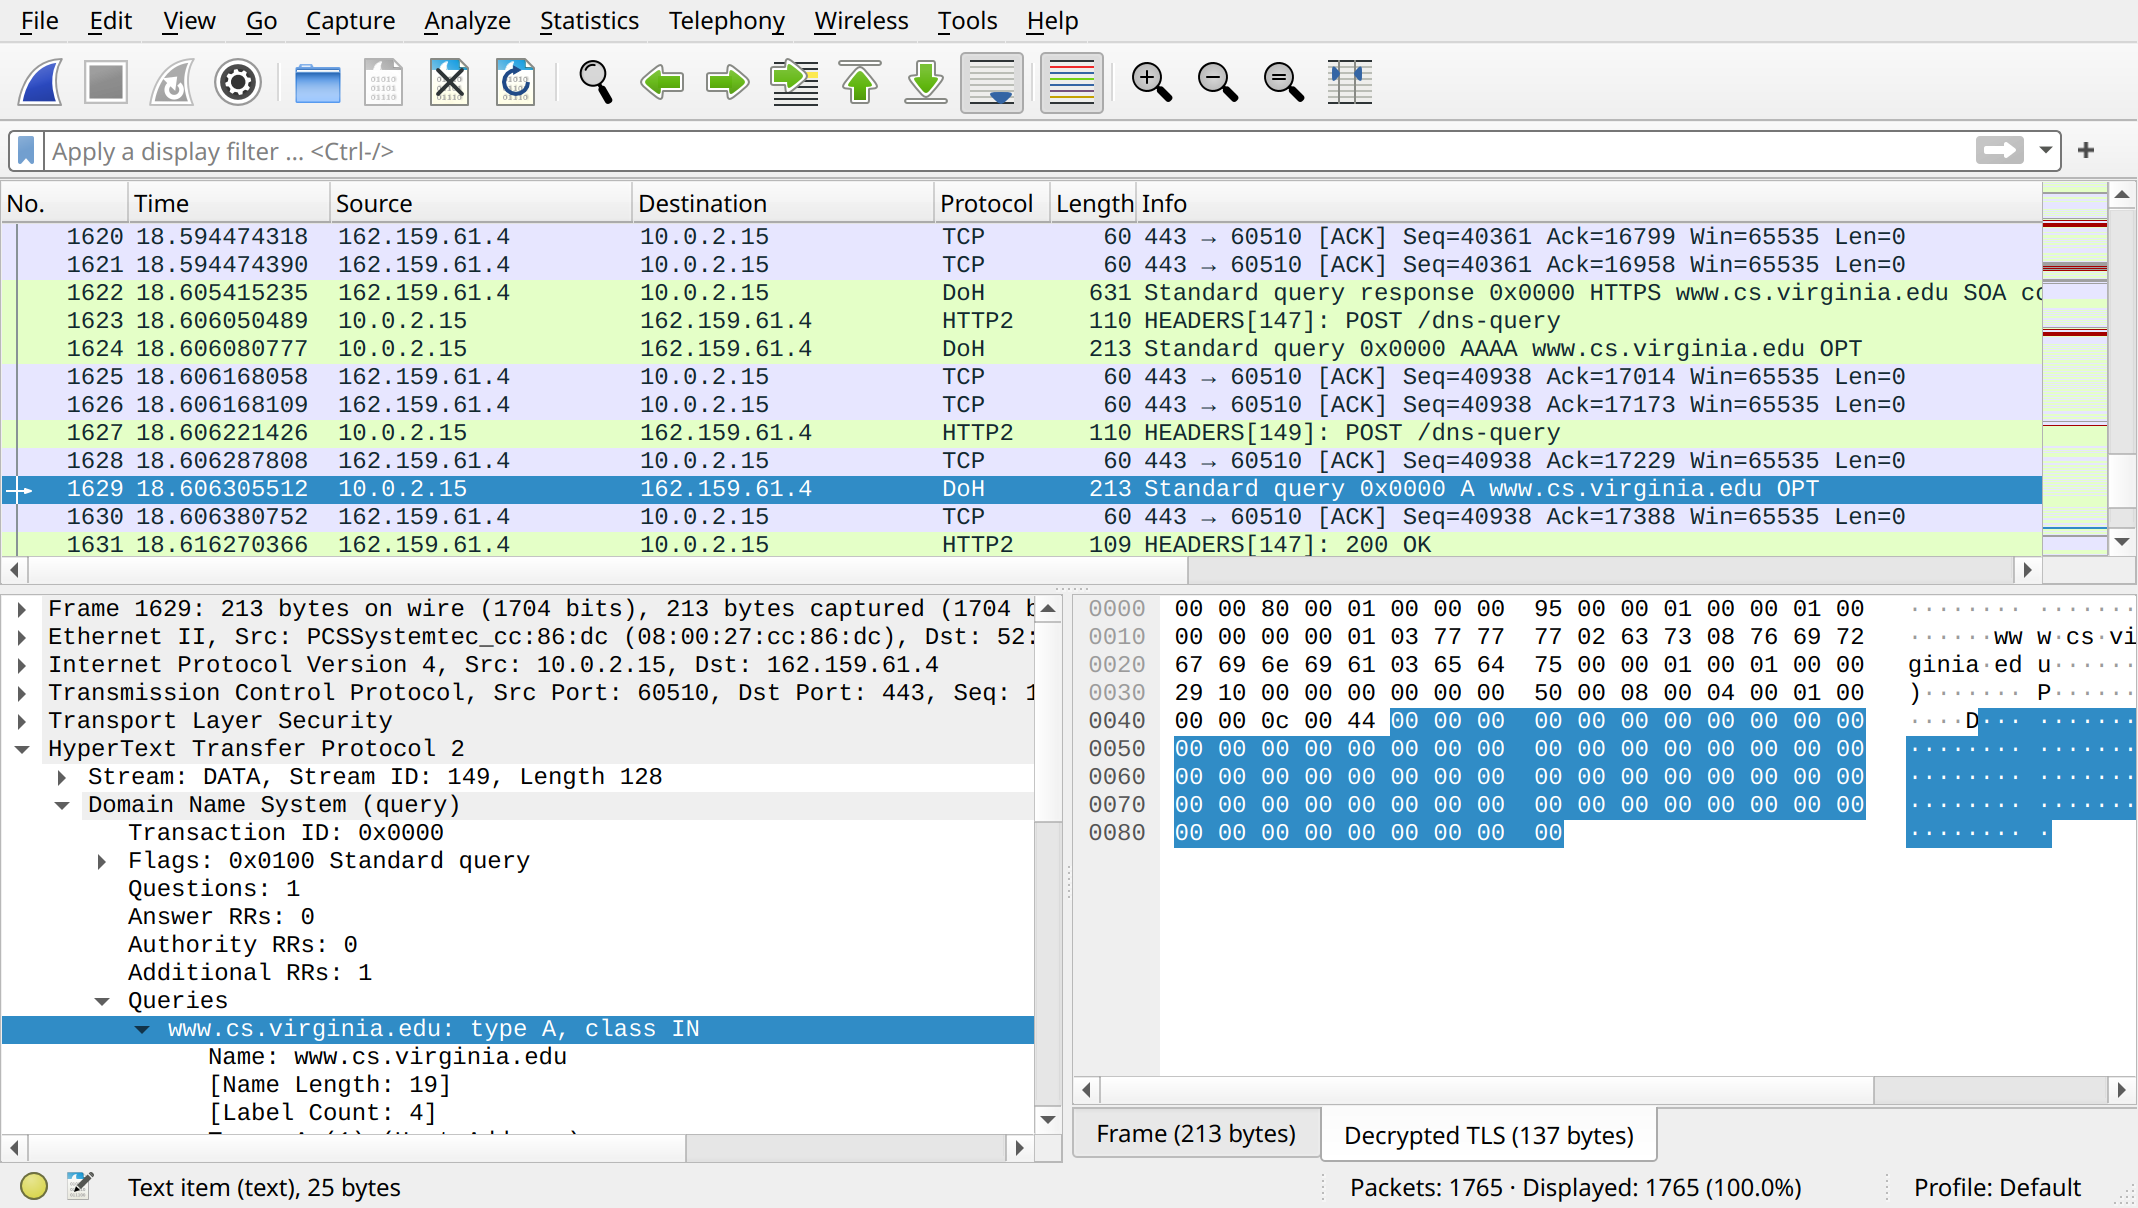
\includegraphics[width=\textwidth]{../intro/wireshark-doh-zoom.png}
};
\path (0, 0) rectangle (14.5, -7); % for bounding box
%\draw[overlay,help lines] (0, 0) grid (14, -8);
    \begin{scope}
        \begin{pgfinterruptboundingbox}
    \tikzset{invclip/.style={clip,insert path={{[reset cm]
          (-16383.99999pt,-16383.99999pt) rectangle (16383.99999pt,16383.99999pt)
      }}}}
        \path[invclip] (6.3, -3.2) rectangle (7.15, -3.4);
        \end{pgfinterruptboundingbox}

        \fill[overlay,white,fill opacity=0.8] (0, 0) rectangle (14.5, -1.2);
        \fill[white,fill opacity=0.8] (0, -1.2) rectangle (14.5, -4);
        \fill[white,fill opacity=0.8] (7.25, -4) rectangle (14.5, -7.9);
    \end{scope}
    \path[draw,red,very thick] (0, -4) rectangle (7.25, -7.9);
    \tikzset{
        protomark/.style={Latex-,blue,thick},
        protomark alt/.style={Latex-,violet,thick,dotted},
        protomark brace/.style={blue,thick,decorate,decoration={brace}},
        protomark brace alt/.style={violet,thick,decorate,decoration={brace}},
        protomark label/.style={blue,fill=white,fill opacity=0.9},
    }
    \draw[protomark] (7.25, -4.3) -- ++(1, .2) node[right,protomark label] {ethernet};
    \draw[protomark] (7.25, -4.5) -- ++ (1, -.2) node[right, protomark label] {
                IPv4 (internet protocol version 4)
        };
    \draw[protomark] (7.25, -4.6) -- ++(1, -.6) node[right,protomark label] {
        TCP ({\fontsize{10}{11}\selectfont transmission control protocol})
    };
    \draw[protomark] (7.25, -4.8) -- ++(1, -1) node[right,protomark label] {
        TLS ({\fontsize{10}{11}\selectfont transport layer security})
    };
    \draw[protomark brace] (7.3, -5) -- (7.3, -7.9);
        \draw[protomark] (7.4, -6.5) -- ++ (0.75, 0) node[right, protomark label] {
            HTTP/2 ({\fontsize{10}{11}\selectfont hypertext transfer protocol 2})
        };
    \draw[protomark brace alt] (7.5, -5.5) -- (7.5, -7.9);
        \draw[protomark alt] (7.6, -6.85) -- ++ (0.75, -.5) node[right, protomark label] {
            DNS (domain name system)
        };
    \draw[red, very thick] (6.3, -3.2) rectangle (7.15, -3.4);
    \draw[red,Latex-,very thick] (7.15, -3.3) -- ++(1, 0) node[right,align=left,overlay box] {
        DoH = DNS over HTTPS
    };
\end{tikzpicture}
\end{frame}

\begin{frame}[fragile]{}
\providecommand{\doHilite}[6]{
    %\doHilite{Y offset start protocol list}{Y offset end protocol list}
    %         {X offset corner data}{Y offset corner data}
    %         {X offset other corner data}{Y offset other corner data}
    \path[draw,red,very thick] (0, -3.95 - #1 * 0.206) rectangle (7.25, -3.95 - #2 * 0.206);
    \path[draw,red,very thick] (7.95 + #3, -4.2059 - #4 * 0.2059) -- (7.95 + #3, -3.95 - #4 * 0.2059)
            -- (12.8, -3.95 - #4 * 0.2059)
            |- (7.95 + #5, -4 - #6 * 0.2059) 
            |- (7.95, -4 - #6 * 0.2059 - .2059) |- cycle;
}
\providecommand{\doHiliteOneDataLine}[6]{
    %\doHilite{Y offset start protocol list}{Y offset end protocol list}
    %         {X offset corner data}{Y offset corner data}
    %         {X offset other corner data}{Y offset other corner data}

    \path[draw,red,very thick] (0, -3.95 - #1 * 0.207) rectangle (7.25, -4 - #2 * 0.207);
    \path[draw,red,very thick] (7.95 + #3, -4.207 - #4 * 0.207) -- (7.95 + #3, -4 - #4 * 0.207)
            %-- (12.8, -4 - #4 * 0.207)
            |- (7.95 + #5, -4 - #6 * 0.207) 
            |- (7.95, -4 - #6 * 0.207 - .207) |- cycle;
}
\begin{tikzpicture}
\tikzset{
    overlay box/.style={fill=white,fill opacity=0.9},
}
\node[overlay,anchor=north west,inner sep=0mm] (base) at (0, 0) {%
\only<1-2>{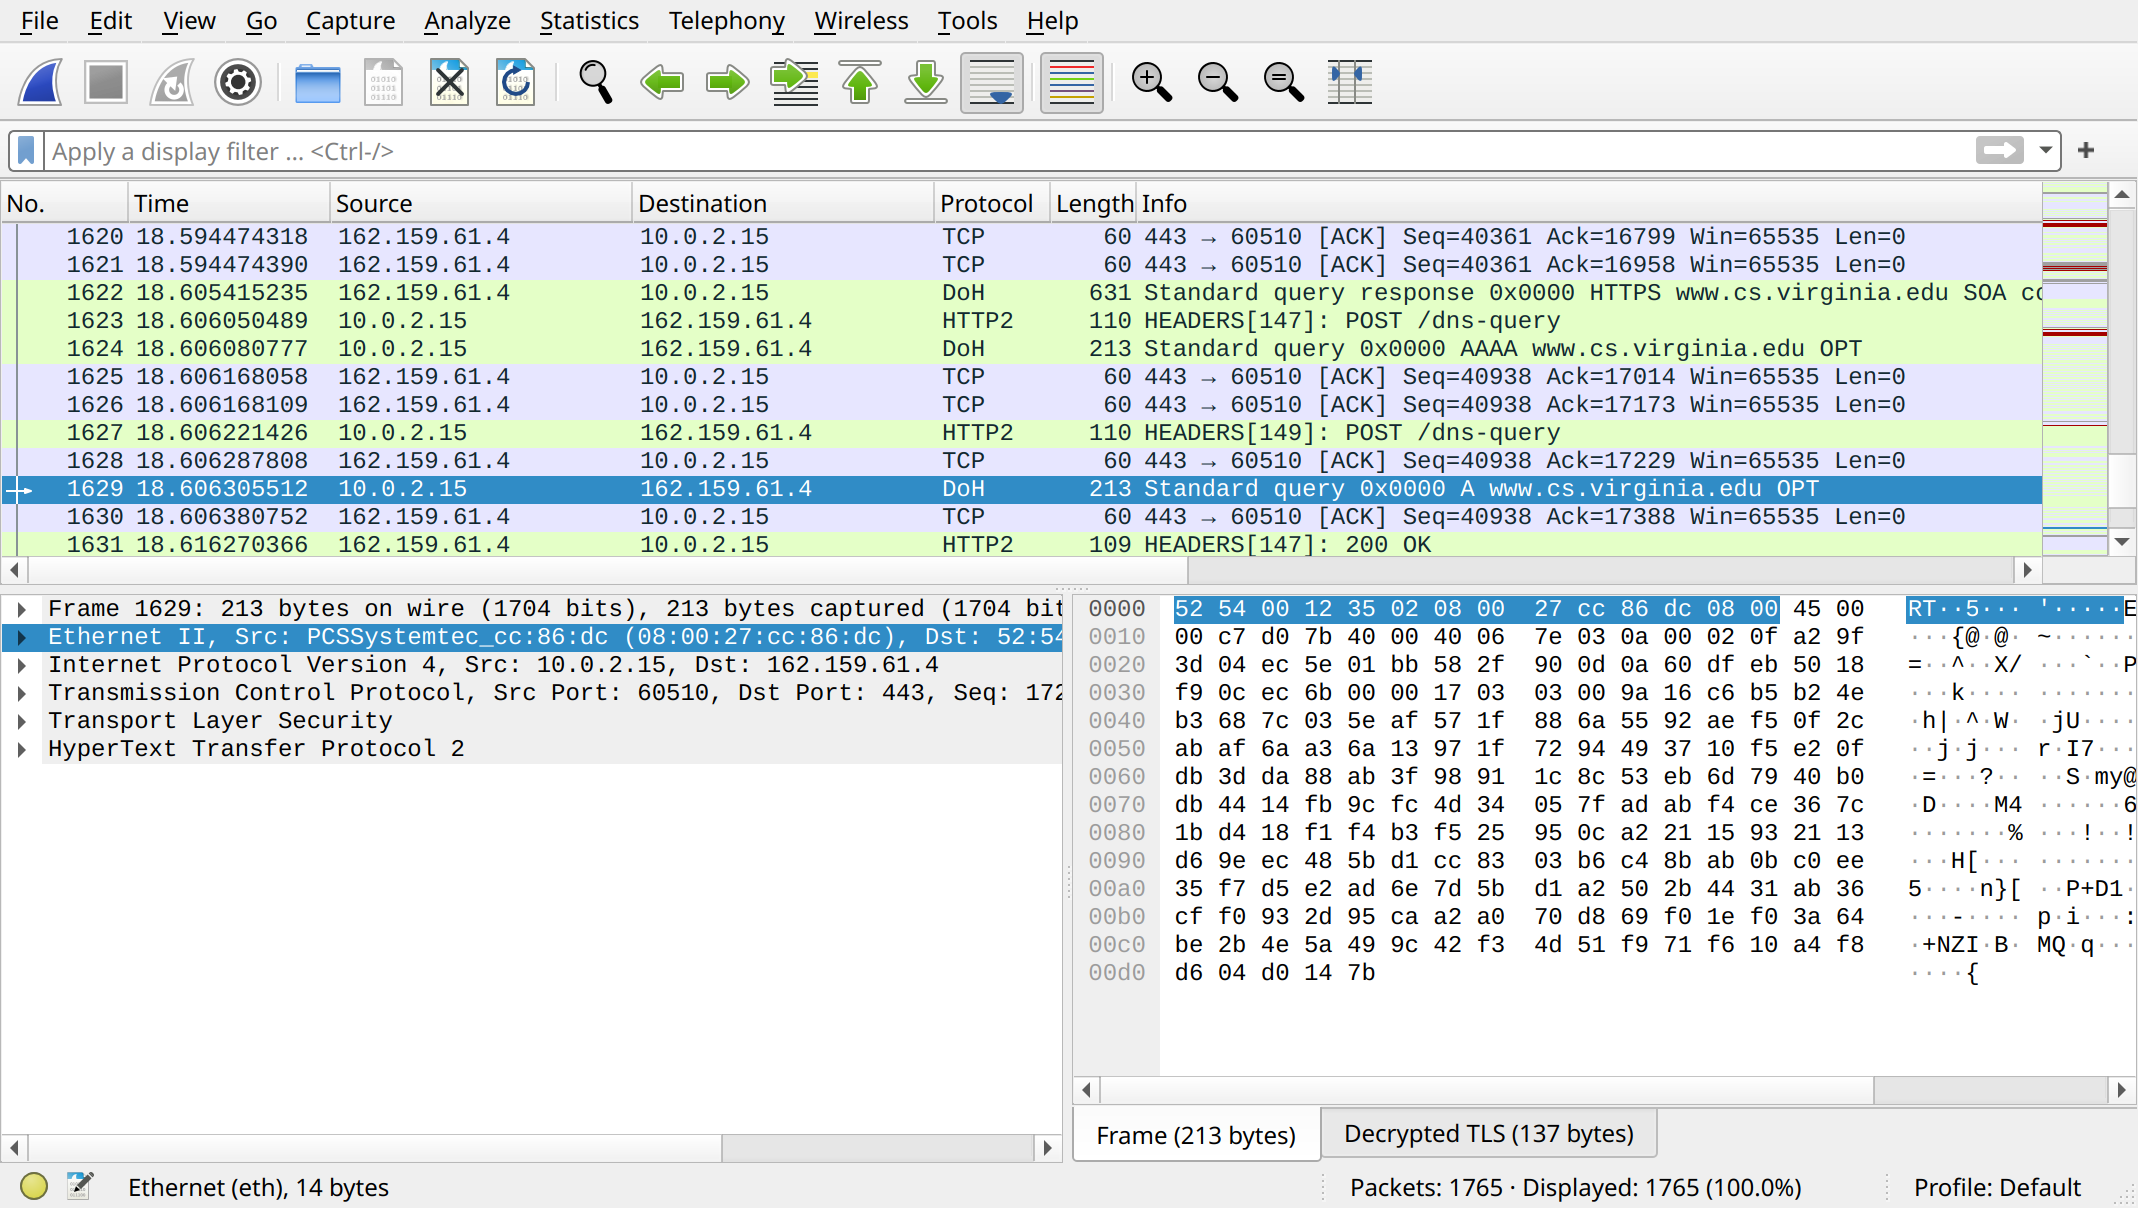
\includegraphics[width=\textwidth]{../intro/wireshark-hi-ethernet.png}}%
\only<3-4>{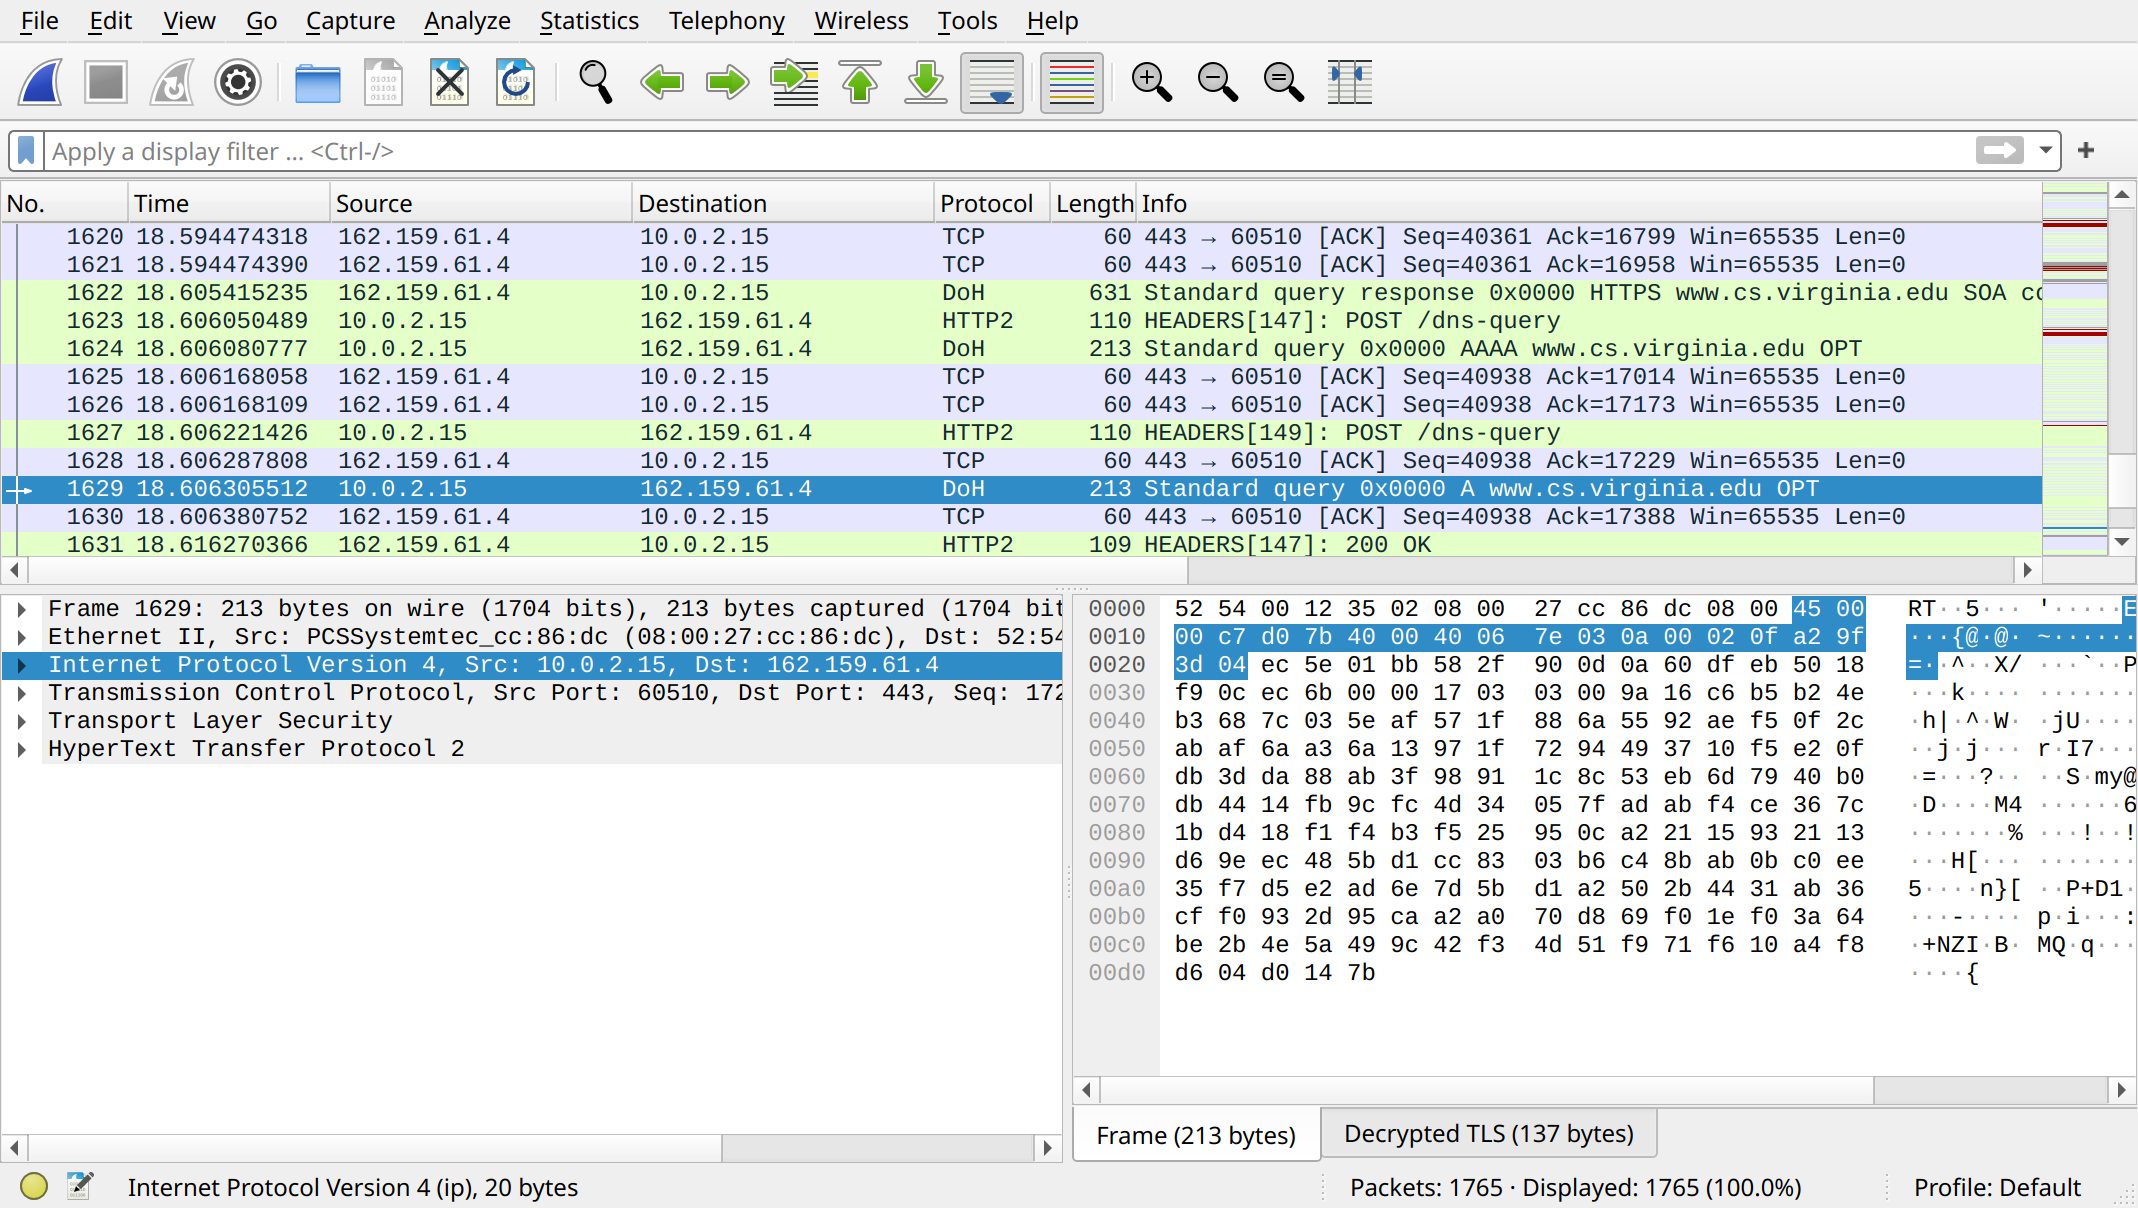
\includegraphics[width=\textwidth]{../intro/wireshark-hi-ipv4.png}}%
\only<5-6>{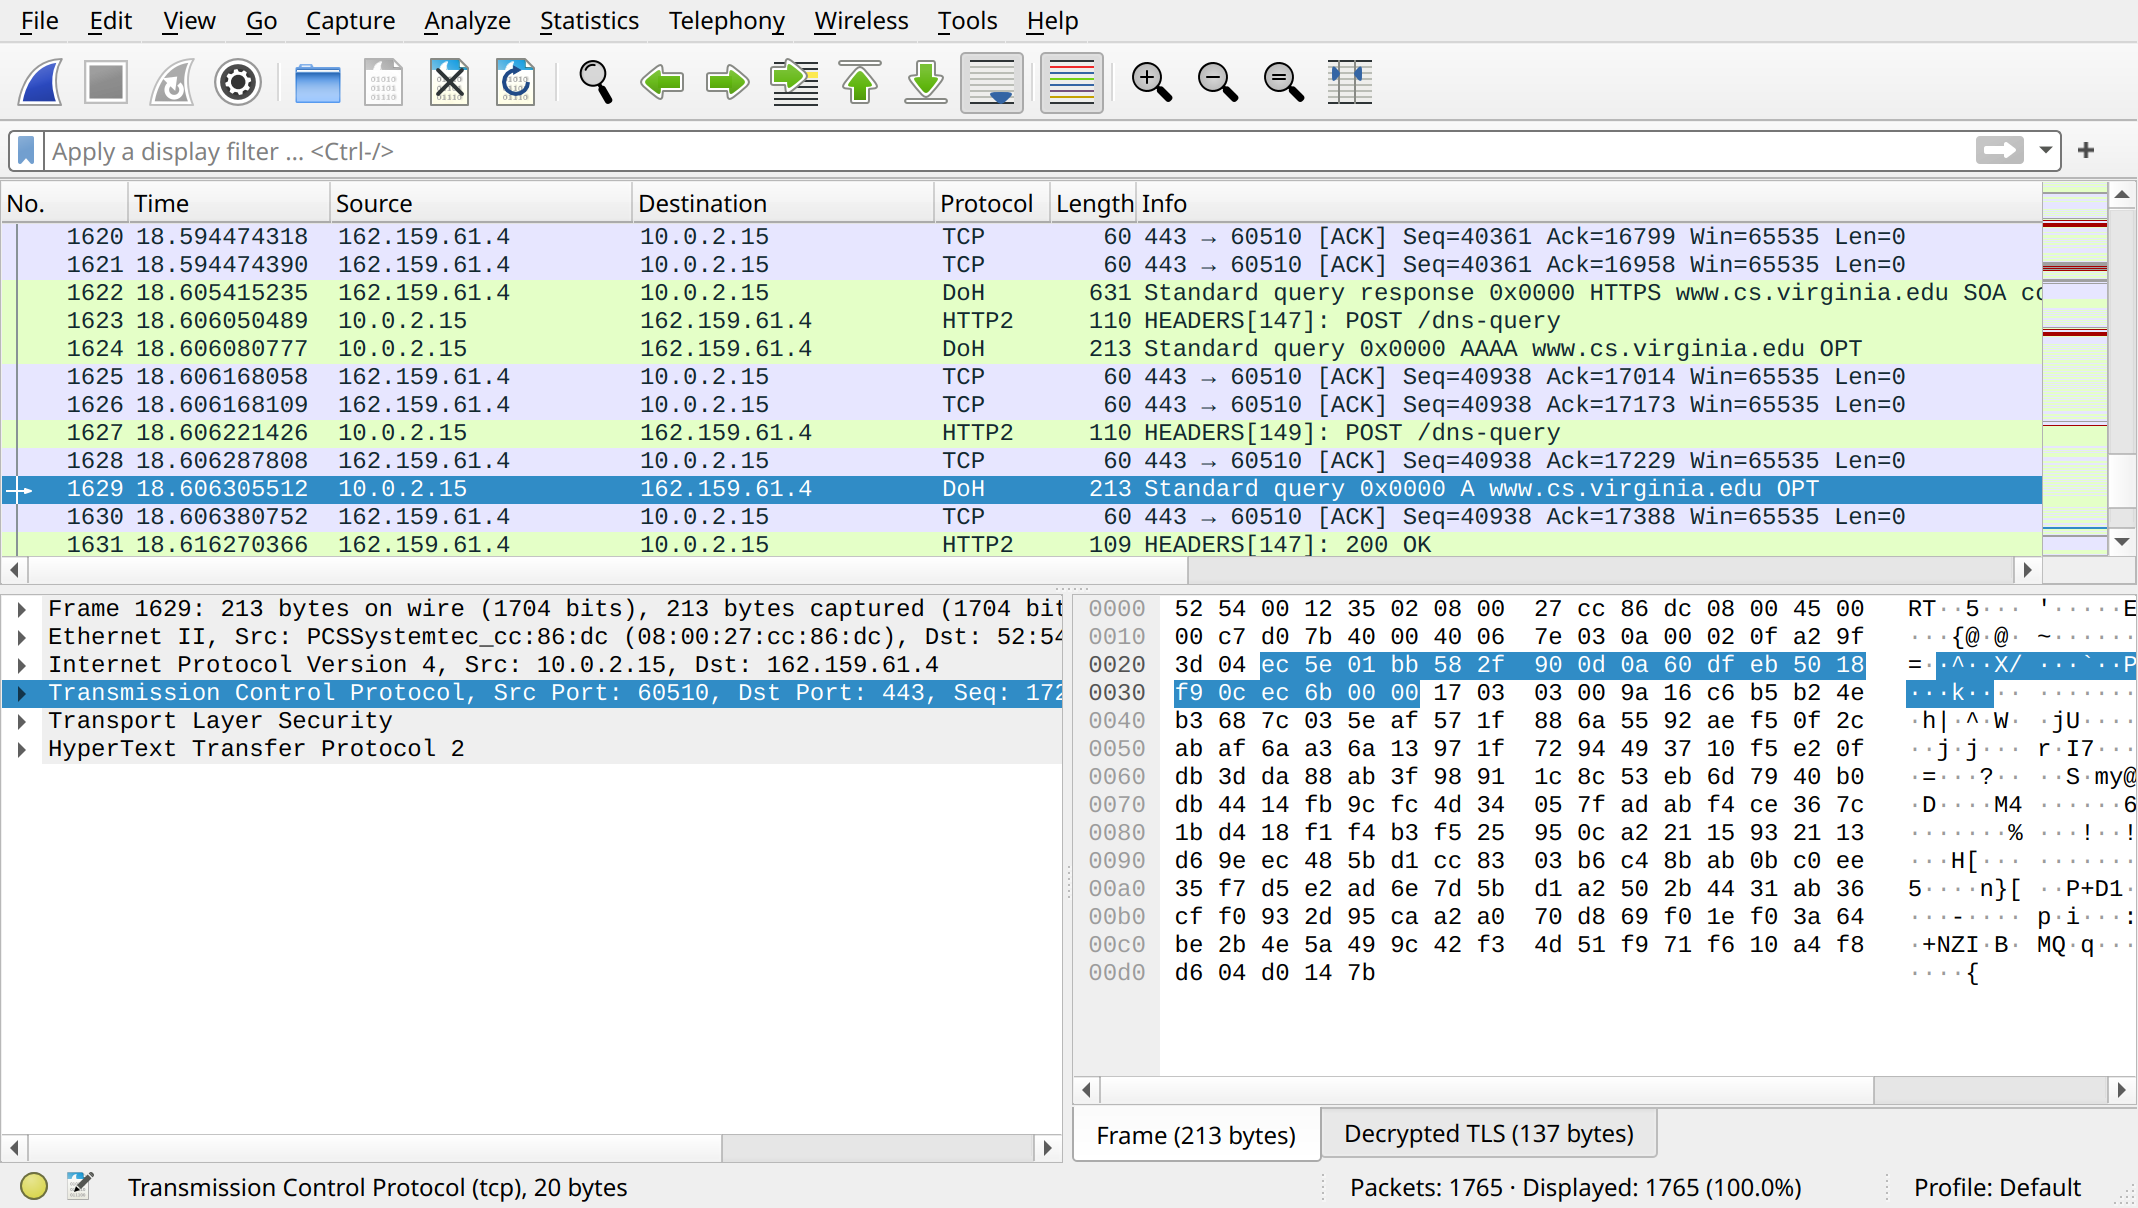
\includegraphics[width=\textwidth]{../intro/wireshark-hi-tcp.png}}%
\only<7-8>{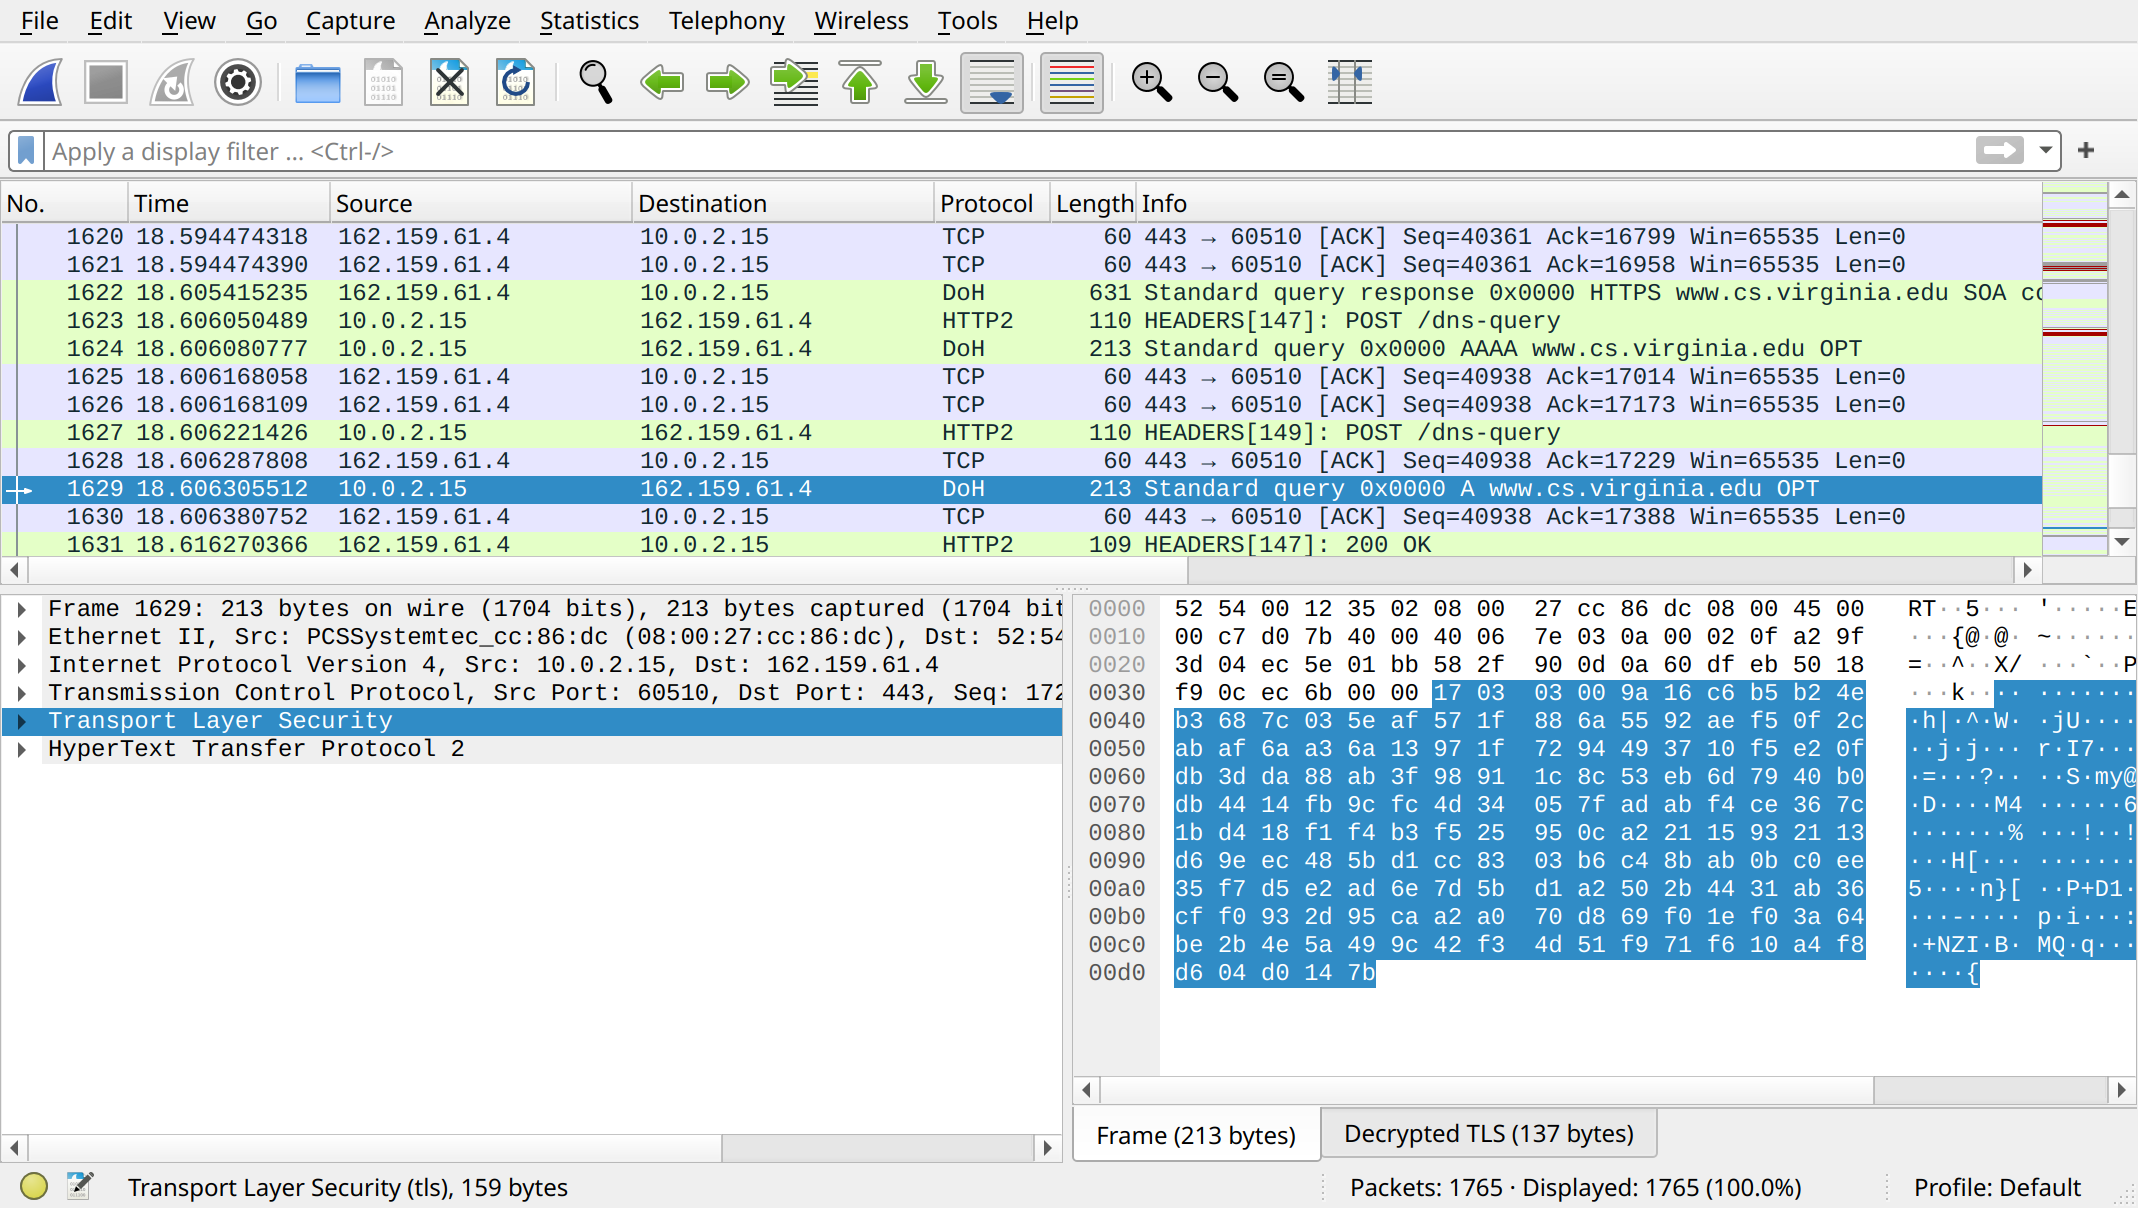
\includegraphics[width=\textwidth]{../intro/wireshark-hi-tls.png}}%
\only<9-11>{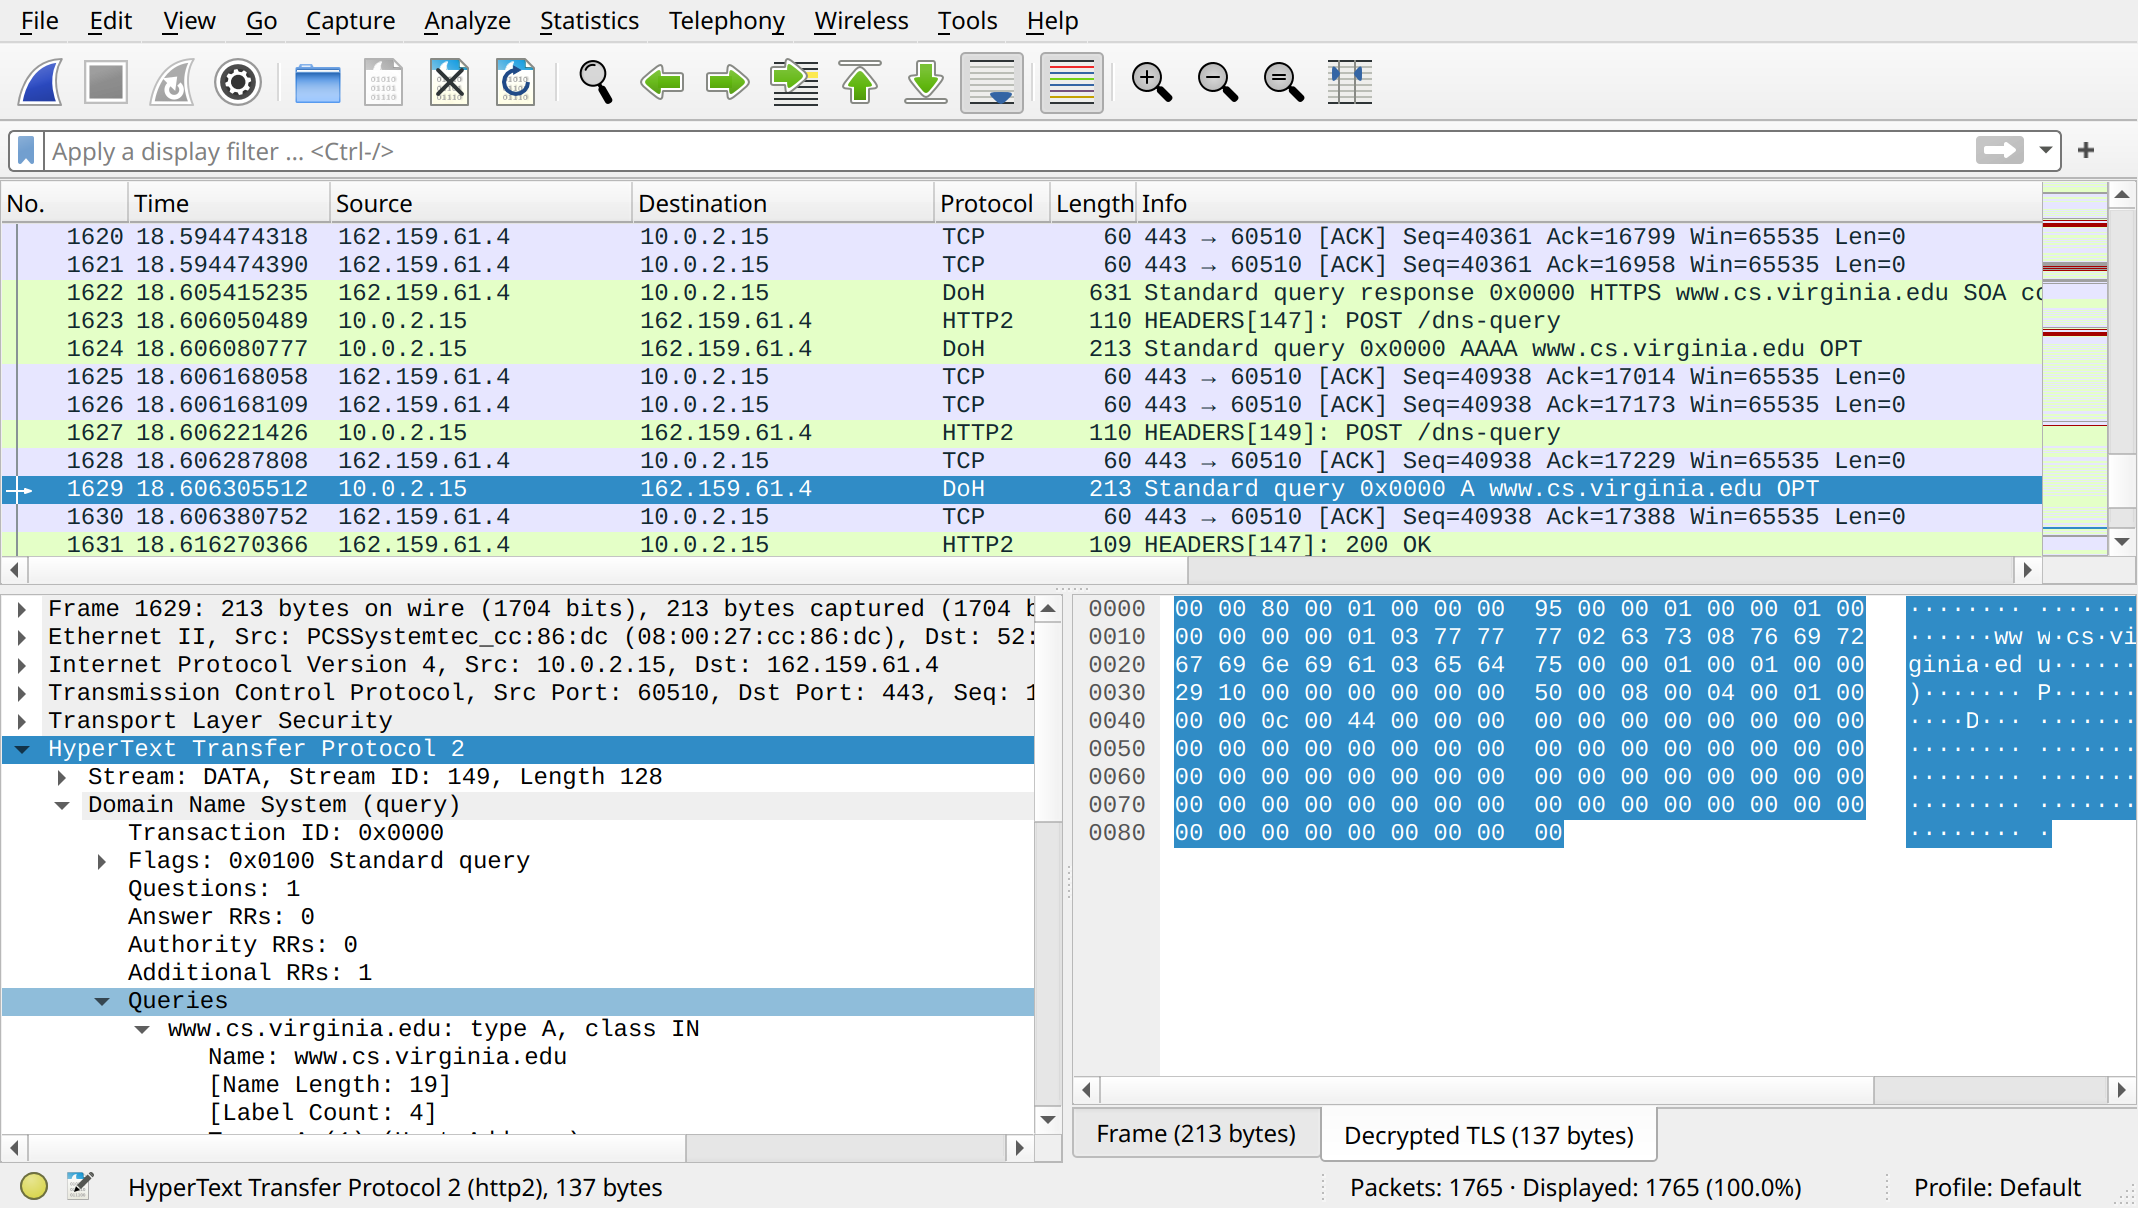
\includegraphics[width=\textwidth]{../intro/wireshark-hi-http.png}}%
\only<12-13>{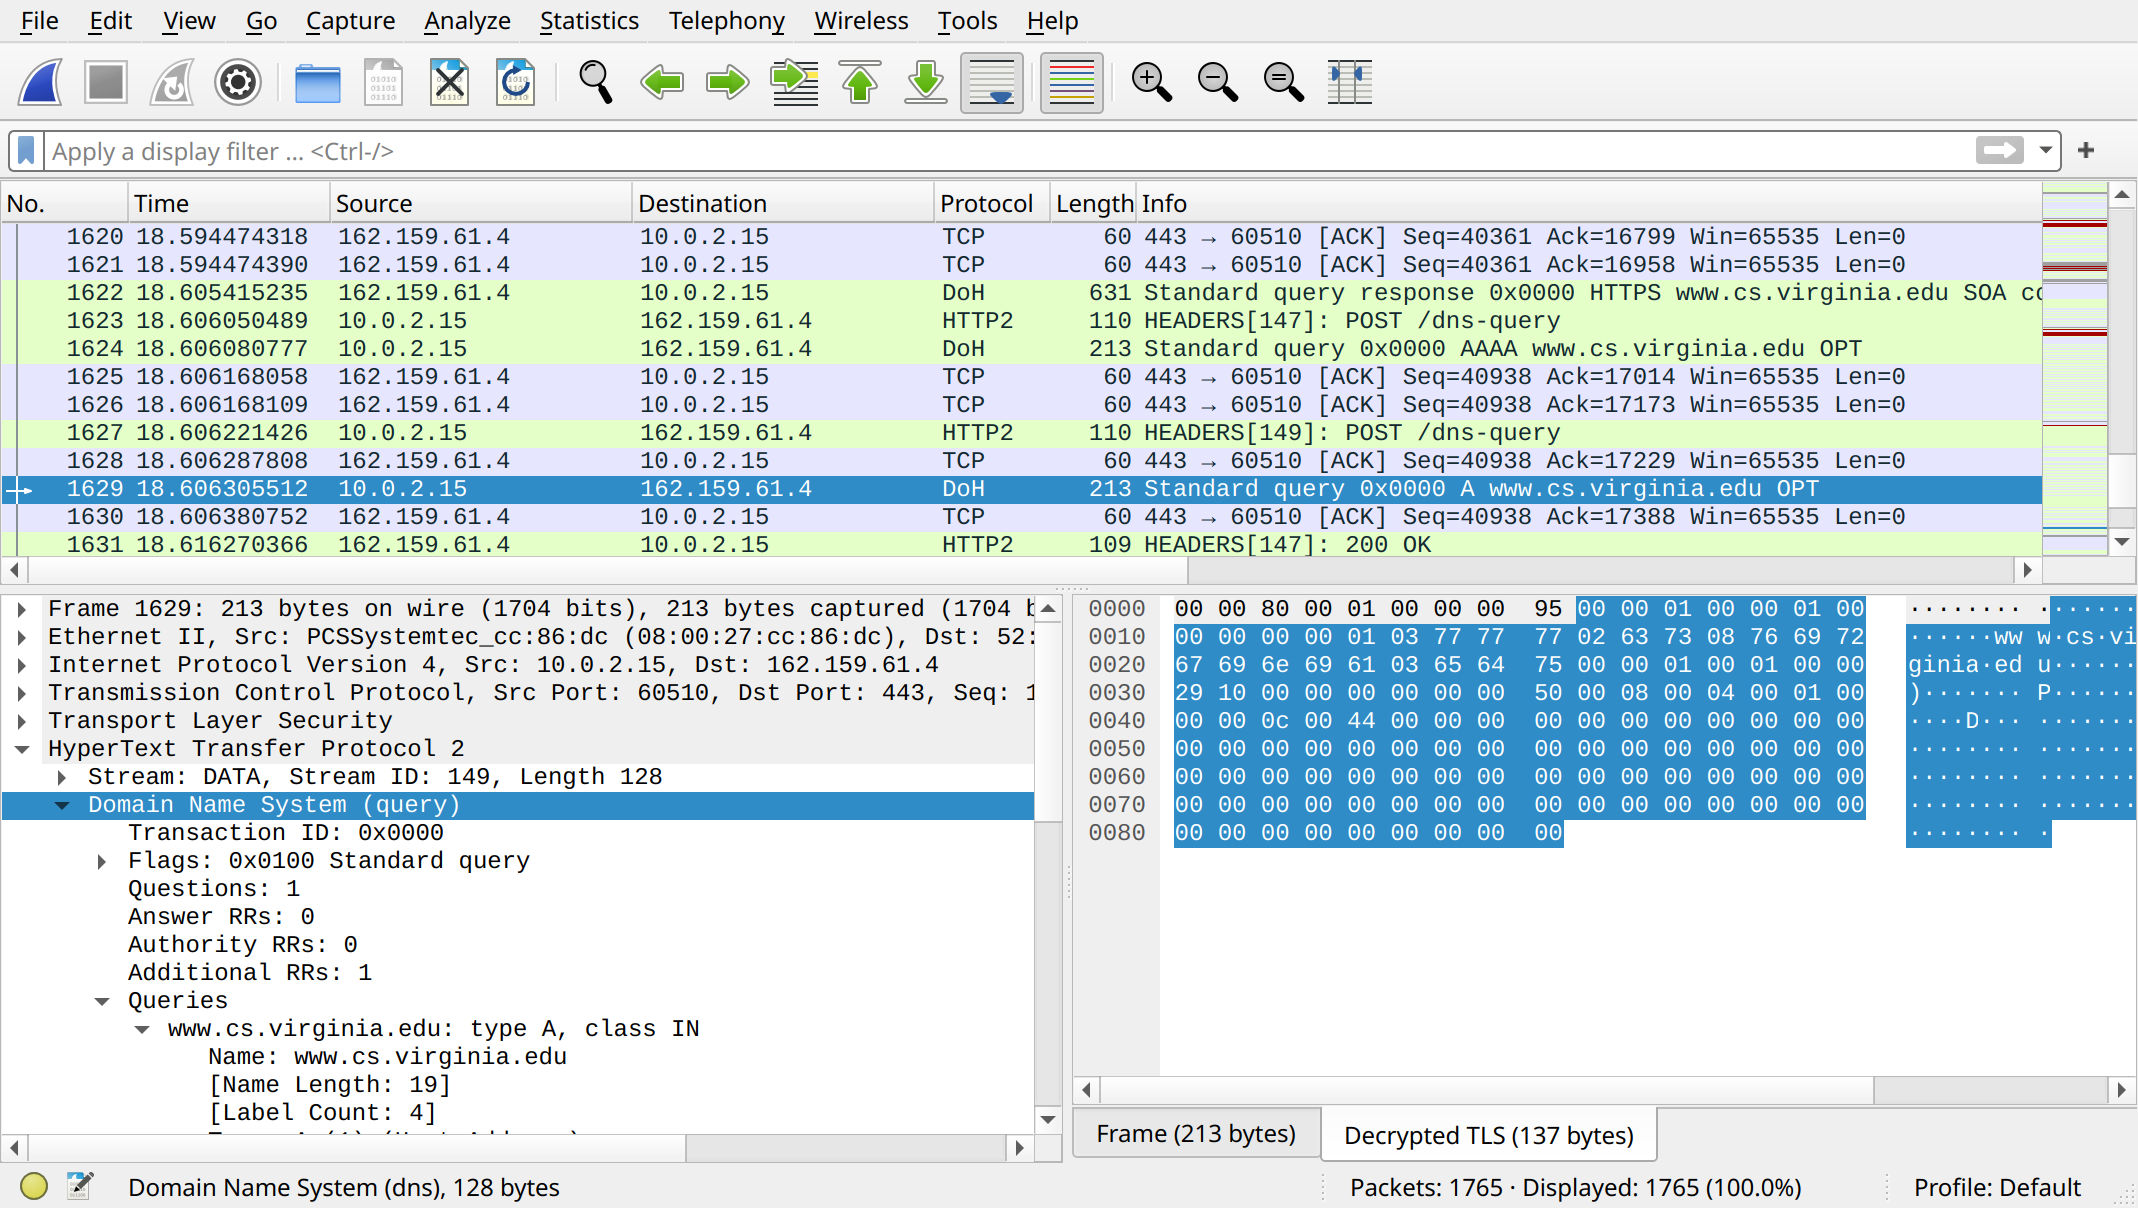
\includegraphics[width=\textwidth]{../intro/wireshark-hi-dns-in-tls.png}}%
};
%\draw[overlay,help lines] (0, 0) grid (14, -8);
\path (0, 0) rectangle (14.5, -7); % for bounding box

\begin{visibleenv}<1> % ethernet
    \doHiliteOneDataLine{1}{2}{0}{0}{4.2}{0}
\end{visibleenv}
\begin{visibleenv}<3> % IP
    \doHilite{2}{3}{4.2}{0}{0.5}{2}
\end{visibleenv}
\begin{visibleenv}<5> % TCP
    \doHilite{3}{4}{0.5}{2}{1.7}{3}
\end{visibleenv}
\begin{visibleenv}<7> % TLS
    \doHilite{4}{5}{1.7}{3}{1.4}{12}
\end{visibleenv}
\begin{visibleenv}<9> % HTTP, decrypted TLS
    \path[draw,red,very thick] (8.9, -7.5) rectangle (11.3, -7.9);
    \node[align=left,overlay box,anchor=south] at (10.4, -7.5) {
        setup step: got Firefox to output \\
        cryptographic keys ({\fontsize{10}{11}\selectfont using \tt SSLKEYLOGFILE})
    };
\end{visibleenv}
\begin{visibleenv}<10> % HTTP
    \doHilite{5}{6}{0}{0}{2.69}{8}
\end{visibleenv}
\begin{visibleenv}<12> % DNS
    \doHilite{7}{8}{2.7}{0}{2.69}{8}
\end{visibleenv}
\end{tikzpicture}
\end{frame}

% FIXME: show multiple related packets --- emphasize filter window
\begin{frame}{}
\begin{tikzpicture}
\tikzset{
    overlay box/.style={fill=white,fill opacity=0.9}
}
\node[overlay,anchor=north west,inner sep=0mm] (base) at (0, 0) {
    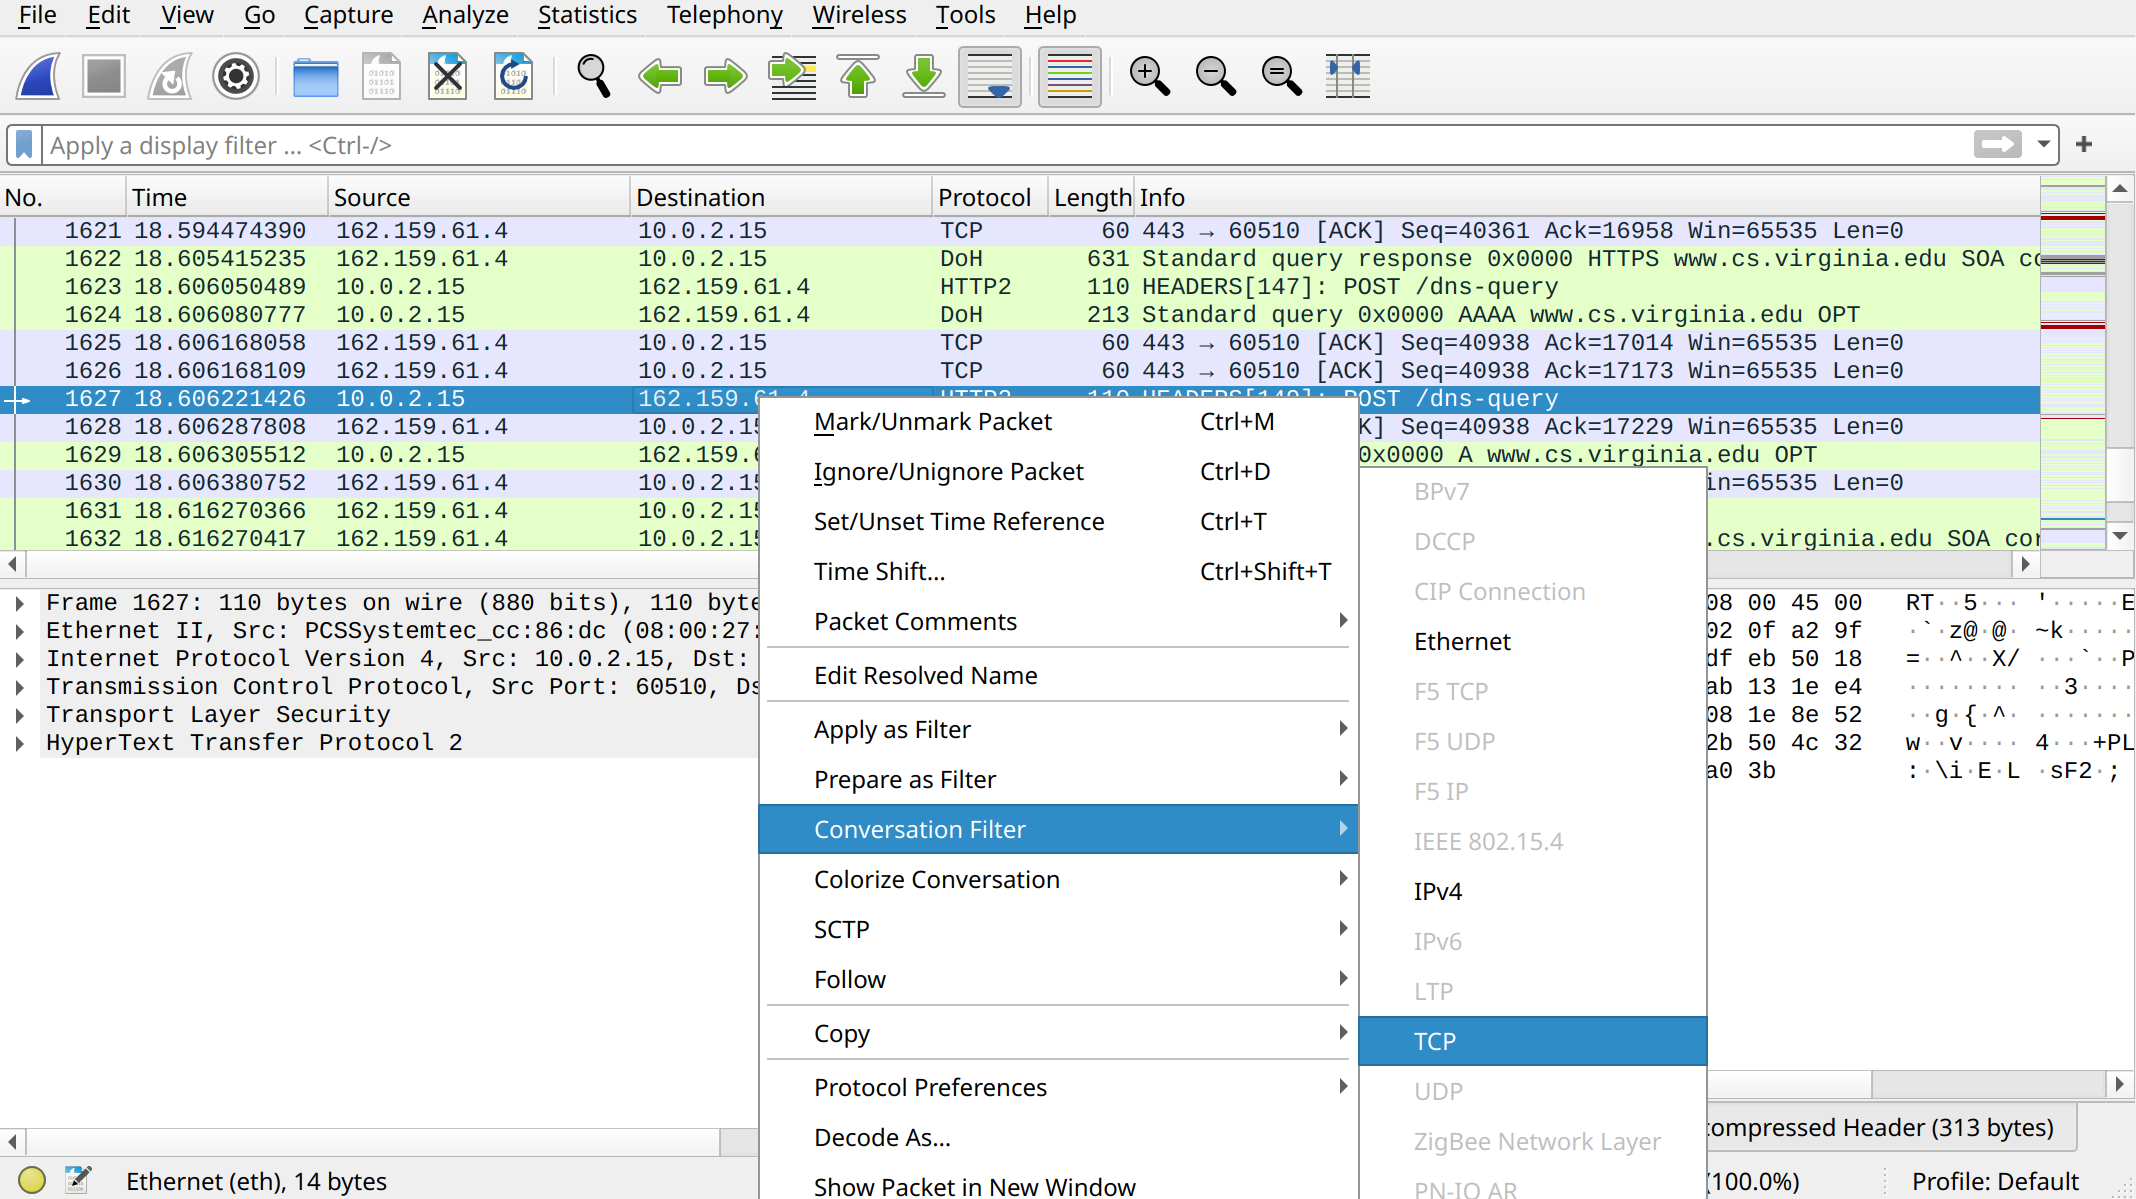
\includegraphics[width=\textwidth]{../intro/wireshark-menu-tcp-filter.png}
};
\path (0, 0) rectangle (14.5, -7); % for bounding box
\end{tikzpicture}
\end{frame}

\begin{frame}{}
\begin{tikzpicture}
\tikzset{
    overlay box/.style={fill=white,fill opacity=0.9}
}
\node[overlay,anchor=north west,inner sep=0mm] (base) at (0, 0) {
    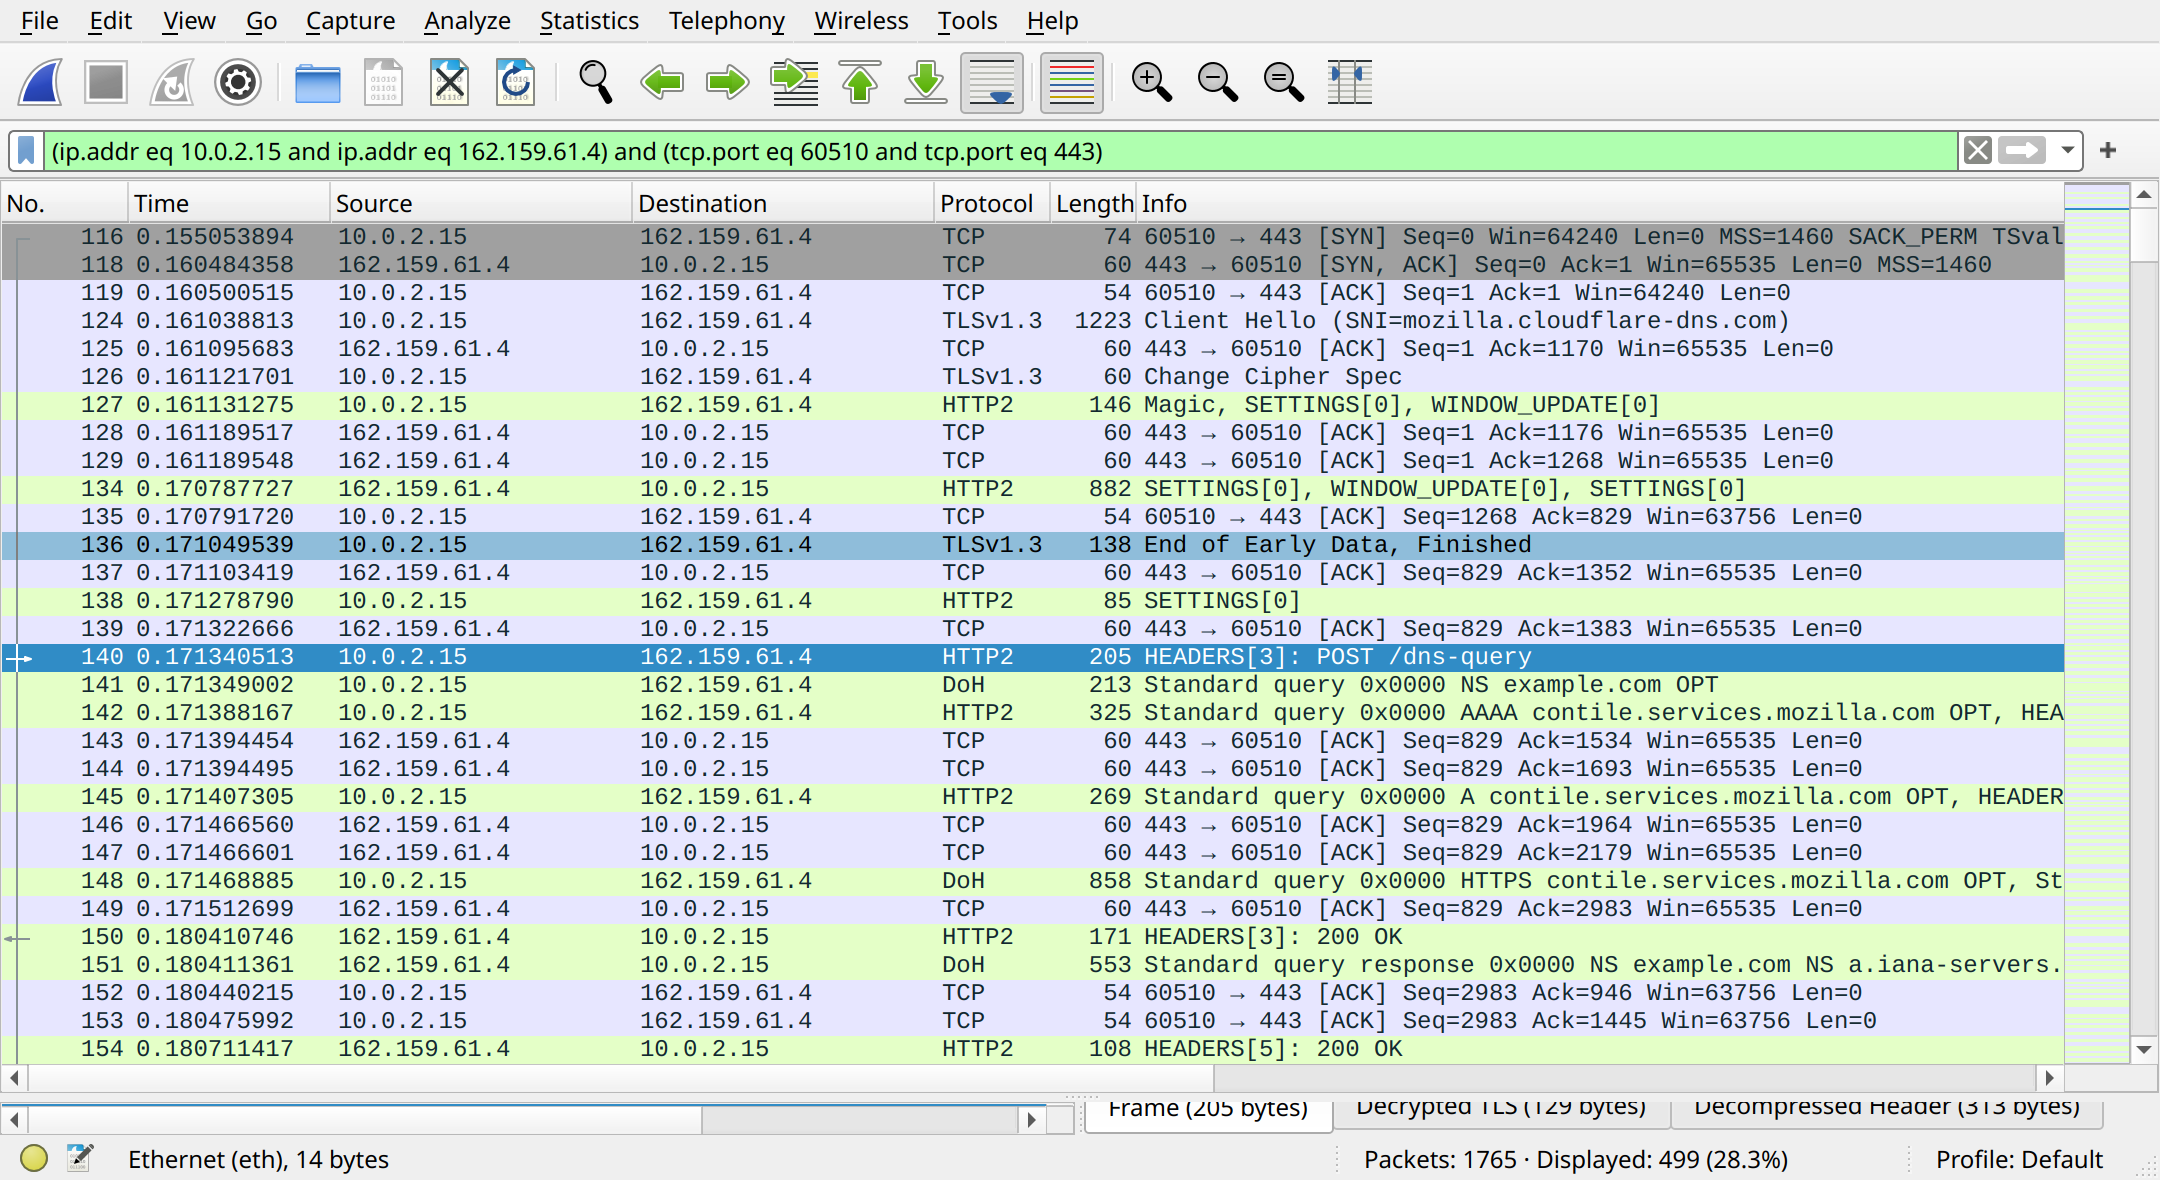
\includegraphics[width=\textwidth]{../intro/wireshark-filtered.png}
};
\path (0, 0) rectangle (14.5, -7); % for bounding box
%\draw[overlay,help lines] (0, 0) grid (14, -8);
%\draw[overlay,help lines,dotted] (0, 0) grid[step=0.2] (14, -8);
\begin{visibleenv}<1>
    \path[draw, red, very thick] (0.3, -0.9) rectangle (13.15, -1.15);
    \node[anchor=north,overlay box,text=red] (filter expr label) at (6.5, -1.15) {
        filter expression 
    };
    \node[anchor=north,overlay box,font=\fontsize{10}{11}\selectfont,align=left] at (filter expr label.south) {
        based on address ($\sim$ machine) and port number ($\sim$ program/socket) fields  \\
        usually means all part of one socket connection
    };
    \path[draw, red, very thick] (10.3, -7.6) rectangle (12.1, -7.9);
    \node[anchor=south,overlay box,text=red] at (11.4, -7.6) {
        499 packets in ``conversation''
    };
\end{visibleenv}
\begin{visibleenv}<2>
    \path[draw,red, very thick] (0, -1.9) rectangle (.85, -2.24);
    \path[draw,red, very thick] (0, -3) rectangle (.85, -3.37);
    \node[overlay box,anchor=west,text=red] at (.85, -2.5) {
        some packets not shown from filter
    };
\end{visibleenv}
\begin{visibleenv}<3>
    \path[draw,red,very thick] (6.25, -1.47) rectangle (7.1, -7.2);
    \node[align=left,overlay box,anchor=south east,text=red] at (6.25, -3) {
        highest layer used \\
        in each packet
    };
    \node[align=left,overlay box,anchor=north east,text=black,font=\fontsize{10}{11}] at (6.25, -3) {
        connection only `for' \\
        DNS over HTTPS (DoH) \\
        but many packets \\
        only needed for \\
        bookkeeping for \\
        the `lower' layers
    };
\end{visibleenv}
\begin{visibleenv}<4>
    \path[draw,red,very thick] (2.2, -1.47) rectangle (6.25, -7.2);
    \node[align=left,overlay box,anchor=west] at (6.25, -4) {
        bookkeeping packets sent \\
        in both directions
    };
\end{visibleenv}
\end{tikzpicture}
\end{frame}



\subsection{end-to-end argument}

\begin{frame}<1>[label=endToEndStatement]{end-to-end argument}
    \begin{itemize}
    \item Saltzer, Reed, Clark, ``End-to-End Arguments in System Design''
    \item ``The function in question can completely and correctly be implemented 
    \myemph<2>{only with the knowledge and help of the application standing at the end points} of the communication
    system. Therefore, providing that questioned function as a feature of the communication
    system itself is not possible. (Sometimes 
    \myemph<3>{an incomplete version of the function provided by the communication system may be useful as a performance enhancement}.)''
    \end{itemize}
\end{frame}

\againframe<2>{endToEndStatement}

\begin{frame}{example: reliable file transfer}
    \begin{itemize}
    \item want to make sure correct data transferred
    \vspace{.5cm}
    \item want to protect against:
        \begin{itemize}
        \item \myemph<2>{error in hardware/software on sending machine reading file}
        \item \myemph<2|3>{bits being flipped in memory on forwarding machine}
        \item communication system flipping bits in data
        \item \myemph<2>{hosts crashing during communication}
        \end{itemize}
    \vspace{.5cm}
    \item<2-> \myemph<2>{\it communication system can't help a lot of these things}
    \item<3-> \myemph<3>{\it authors experienced router with bad memory/processor}
    \end{itemize}
\end{frame}

\begin{frame}{solution: end-to-end checks}
    \begin{itemize}
    \item want reliable transfer: compare final files (with hash or similar)
    \vspace{.5cm}
    \item ``end-to-end'' --- doesn't care what middle systems do
    \end{itemize}
\end{frame}


\againframe<3>{endToEndStatement}

\begin{frame}{end-to-end in practice}
    \begin{itemize}
    \item ``narrow waist'' of IP doesn't provide many gaurnetees
        \begin{itemize}
        \item no gaurentees about reliable transmission, duplicate suppression, message order, \ldots
        \end{itemize}
    \item but try to provide good service (``best effort'')
    \vspace{.5cm}
    \item in design: typically middle systems won't know/care about what's forwarded
        \begin{itemize}
        \item but many exceptions
        \end{itemize}
    \end{itemize}
\end{frame}


\begin{frame}{interlude: quiz}
\end{frame}

\begin{frame}{bits on medium}
    \begin{itemize}
    \item we'll focus on switched networks to start
        \begin{itemize}
        \item deal with problem of sharing medium [much] later
        \end{itemize}
    \item start with: lets say we can send bits on wire/etc.
        \begin{itemize}
        \item subject for first assignment
        \end{itemize}
    \end{itemize}
\end{frame}


\section{framing}

\subsection{aligning the bits}

\usetikzlibrary{fit,matrix}
\begin{frame}{aligning bits}
    \begin{itemize}
    \item let's transmit these (binary) messages:
        \begin{itemize}
        \item \tt 001
        \item \tt 0110
        \item \tt 0010
        \end{itemize}
    \end{itemize}
\begin{tikzpicture}
\matrix[tight matrix no line,nodes={text width=.35cm,font=\large\tt}] (msg) {
|[alias=s1]| 0 \& 0 \& |[alias=e1]| 1 \& |[alias=s2]| 0 \& 1 \& 1 \& |[alias=e2]| 0 \& 
|[alias=s3]| 0 \& 0 \& 1 \& |[alias=e3]| 0 \\
};
\foreach \x in {1,2,3} {
    \node[inner sep=0mm,outer sep=0mm,draw,red,very thick,fit=(s\x) (e\x),alt=<2>{opacity=0.1}] {};
}
\end{tikzpicture}
\begin{itemize}
\item<2-> problem: can't tell where messages/start end
\end{itemize}
\end{frame}


\subsection{size strategy}

\usetikzlibrary{decorations.pathreplacing}
\begin{frame}{size `header'}
\begin{itemize}
    \item let's transmit these (binary) messages:
        \begin{itemize}
        \item \tt 001
        \item \tt 0110
        \item \tt 0010
        \end{itemize}
    \item put 3-bit message size at beginning of messages
\end{itemize}
\begin{tikzpicture}
\matrix[tight matrix no line,nodes={text width=.35cm,font=\large\tt}] (msg) {
|[alias=h1]| 0 \& 1 \& 1 \& |[alias=s1]| 0 \& 0 \& |[alias=e1]| 1 \& 
|[alias=h2]| 1 \& 0 \& 0 \& |[alias=s2]| 0 \& 1 \& 1 \& |[alias=e2]| 0 \& 
|[alias=h3]| 1 \& 0 \& 0 \& |[alias=s3]| 0 \& 0 \& 1 \& |[alias=e3]| 0 \\
};
\foreach \x in {1,2,3} {
    \node[inner sep=0mm,outer sep=0mm,draw,green,very thick,fit=(s\x) (e\x)] {};
    \node[inner sep=0mm,outer sep=0mm,fill=blue,fill opacity=0.1,very thick,fit=(h\x) (s\x.west)] {};
    \draw[very thick,decorate,decoration={brace,mirror}] 
        ([xshift=.1cm,yshift=-.1cm]h\x.south west) -- ([xshift=-.1cm,yshift=-.1cm]e\x.south east) {};
}
\end{tikzpicture}
\begin{itemize}
\item read header, then determine number of bits to read before next header
\item<2-> assumption: \myemph<2>{no gaps between messages?}
    \begin{itemize}
    \item need to transmit \textit{something} in between messages
    \end{itemize}
\end{itemize}
\end{frame}



\subsection{start/end symbol strategy}

\begin{frame}{start/end symbol}
    \begin{itemize}
    \item alternate idea: use bit sequence to mark beginning/end
    \item example choice: send 010 between each frame
    \item send extra 010s when no frames to send
    \end{itemize}
\begin{tikzpicture}
\matrix[tight matrix no line,nodes={text width=.35cm,font=\large\tt}] (msg) {
|[alias=h1]| 0 \& 1 \& 0 \& |[alias=s1]| 0 \& |[alias=bform1s]| 0 \& |[alias=e1,alias=bform1e]| 1 \& 
|[alias=h2]| 0 \& 1 \& 0 \& |[alias=s2,alias=bform2s]| 0 \& |[alias=bform2e]| 1 \& 1 \& |[alias=e2]| 0  \&
|[alias=h3]| 0 \& 1 \& 0 \& |[alias=s3]| 0 \& |[alias=false start,alias=bform3s]| 0 \& |[alias=bform3e]| 1 \& |[alias=e3,alias=false end]| 0 \& |[alias=h4]| 0 \& 1 \& 0 \& |[alias=s4]| ~ \\
};
\foreach \x in {1,2,3} {
    \node[inner sep=0mm,outer sep=0mm,draw,green,alt=<2>{opacity=0.1},very thick,fit=(s\x) (e\x)] {};
}
\foreach \x in {1,2,3,4} {
    \node[inner sep=0mm,outer sep=0mm,fill=blue,fill opacity=0.1,alt=<3>{fill opacity=0.05},very thick,fit=(h\x) (s\x.west)] {};
}
\foreach \x in {1,2,3} {
    \draw[very thick,decorate,decoration={brace,mirror}] 
        ([xshift=.1cm,yshift=-.1cm]s\x.south west) -- ([xshift=-.1cm,yshift=-.1cm]e\x.south east) {};
    \begin{visibleenv}<3>
    \fill[fill opacity=0.1,red,draw=violet,ultra thick,dotted] (bform\x s.south west) rectangle (bform\x e.north east);
    \end{visibleenv}
}
\begin{visibleenv}<2>
\node[draw=red,ultra thick,fit=(false start) (false end),inner sep=1mm,outer sep=0mm] {};
\end{visibleenv}
\end{tikzpicture}
\begin{itemize}
\item<2-> problem: \myemph<2>{messages can contain \texttt{010} or end with \texttt{01}}
\item<3-> one solution: replace \texttt{01} in messages with \texttt{011}
    \begin{itemize}
    \item (need to undo replacement when receiving)
    \end{itemize}
\end{itemize}
\begin{visibleenv}<3->
\begin{tikzpicture}
\matrix[tight matrix no line,nodes={text width=.35cm,font=\large\tt}] (msg) {
|[alias=h1]| 0 \& 1 \& 0 \& |[alias=s1]| 0 \& |[alias=xform1s]| 0 \& 1 \& |[alias=xform1e,alias=e1]| 1 \&  
|[alias=h2]| 0 \& 1 \& 0 \& |[alias=s2,alias=xform2s]| 0 \& 1 \& |[alias=xform2e]| 1 \& 1 \& |[alias=e2]| 0 \&
|[alias=h3]| 0 \& 1 \& 0 \& |[alias=s3]| 0 \&|[alias=xform3s]| 0 \& 1 \& |[alias=xform3e,alias=e3]| 1 \& |[alias=e3]| 0 \& |[alias=h4]| 0 \& 1 \& 0 \& |[alias=s4]| ~ \\
};
\foreach \x in {1,2,3} {
    \node[inner sep=0mm,outer sep=0mm,draw,green,alt=<2>{opacity=0.1},very thick,fit=(s\x) (e\x)] {};
}
\foreach \x in {1,2,3,4} {
    \node[inner sep=0mm,outer sep=0mm,fill=blue,fill opacity=0.1,alt=<3>{fill opacity=0.05},very thick,fit=(h\x) (s\x.west)] {};
}
\foreach \x in {1,2,3} {
    \draw[very thick,decorate,decoration={brace,mirror}] 
        ([xshift=.1cm,yshift=-.1cm]s\x.south west) -- ([xshift=-.1cm,yshift=-.1cm]e\x.south east) {};
    \fill[fill opacity=0.1,red,draw=violet,ultra thick,dotted] (xform\x s.south west) rectangle (xform\x e.north east);
}
\end{tikzpicture}
\end{visibleenv}
\end{frame}

\begin{frame}[fragile]{escaping?}
    \begin{itemize}
    \item can think of replacement similar to escaping strings in C
        \begin{itemize}
        \item start/end marker is \verb|"|
        \item \verb|"| $\rightarrow$ \verb|\"|
        \item \verb|\| $\rightarrow$ \verb|\\|
        \end{itemize}
    \item represent \verb|foo \R"3"13\| using \verb|"foo \\R\"3\"13\\"|
    \item but needed tweaks to idea to work with bits instead of bytes
    \vspace{.5cm}
    \item<2-> some physical layers allow transmitting bytes at a time
    \item<2-> example: upcoming assignment
    \item<2-> framing protocols for those (example: PPP) use \textbackslash-like idea
    \end{itemize}
\end{frame}

\begin{frame}{help from physical layer?}
    \begin{itemize}
    \item suppose instead of transmitting 0 or 1
    \item \ldots physical layer transmits 0 or 1 or 2 or 3 or 4
    \item probably going to `waste' one of these values
        \begin{itemize}
        \item example: transmit every two bits as 0 or 1 or 2 or 3
        \end{itemize}
    \vspace{.5cm}
    \item<2-> idea: take advantage of leftover `symbol' 4
    \item<2-> use it to send start/end
        \begin{itemize}
        \item similar idea used in many versions of Ethernet
        \end{itemize}
    \end{itemize}
\end{frame}


\subsection{aside: start/end ambiguity}
\begin{frame}{bad choice of start/end (1)}
    \begin{itemize}
    \item [this slide added 6 Sep 2024]
    \item let's say we choose delimiter \texttt{0000}
    \item what do we need to escape?
    \end{itemize}
\begin{tabular}{l}
A. any 0000 \\
A. any 000 \\
B. any 00 \\
C. any 0 \\
\end{tabular}
\end{frame}

\begin{frame}{bad choice of start/end (1)}
    \begin{itemize}
    \item sending \texttt{10} and \texttt{01}
        \begin{itemize}
        \item {\tt \myemph{10}0000\myemph{01}0000}
        \end{itemize}
    \item sending \texttt{1} and \texttt{001}
        \begin{itemize}
        \item {\tt \myemph{1}0000\myemph{001}0000}
        \end{itemize}
    \vspace{.5cm}
    \item oops!
    \item textbook example: start/end = {\tt 01111110}
    \end{itemize}
\end{frame}



\subsection{types of transmission errors}

% FIXME: worth keeping?
\begin{frame}<1>[label=transmitErrorType]{types of transmission errors}
    \begin{itemize}
    \item \myemph<2>{desynchronization}:
        \begin{itemize}
        \item missing bits/bytes
        \item adding bits/bytes
        \end{itemize}
    \item \myemph<3>{flipping bits}
        \begin{itemize}
        \item from `noise'/`interference'
        \end{itemize}
    \end{itemize}
\end{frame}

\againframe<2>{transmitErrorType}

\begin{frame}{desynchronization and framing (1)} 
    \begin{itemize}
    \item with purely size-based framing 
        \begin{itemize}
        \item almost all future sizes messed up
        \end{itemize}
    \end{itemize}
\begin{tikzpicture}
\tikzset{
    disappears/.style={opacity=0.1},
}
\matrix[tight matrix no line,nodes={text width=.35cm,font=\large\tt,name prefix=norm-}] (msg) {
|[alias=h1]| 0 \& 1 \& 1 \& |[alias=s1]| 0 \& 1 \& |[alias=e1]| 0 \& 
|[alias=h2]| 1 \& 0 \& 0 \& |[alias=s2]| 0 \& 1 \& 1 \& |[alias=e2]| 0 \& 
|[alias=h3]| 1 \& 0 \& 0 \& |[alias=s3]| 0 \& 1 \& 1 \& |[alias=e3]| 1 \& \ldots \& ~ \& \ldots \\
};
\matrix[anchor=north west,tight matrix no line,nodes={text width=.35cm,font=\large\tt,name prefix=bad-}] (msg alt)
at ([yshift=-1cm]msg.south west) {
|[disappears]| \sout{0} \& |[alias=h1]| 1 \& 1 \& 0 \& |[alias=s1]| 1 \& 0 \& 
1 \& 0 \& 0 \& |[alias=e1]| 0 \& |[alias=h2]| 1 \& 1 \& 0 \& 
|[alias=s2]| 1 \& 0 \& 0 \& 0 \& 1 \& |[alias=e2]| 1 \& |[alias=h3]| 1 \& |[alias=s3]| \ldots \& |[alias=e3]| ~ \& \ldots \\
};
\foreach \x in {1,2,3} {
    \foreach \pfx in {norm,bad} {
        \node[inner sep=0mm,outer sep=0mm,draw,green,very thick,fit=(\pfx-s\x) (\pfx-e\x)] {};
        \node[inner sep=0mm,outer sep=0mm,fill=blue,fill opacity=0.1,very thick,fit=(\pfx-h\x) (\pfx-s\x.west)] {};
        \draw[very thick,decorate,decoration={brace,mirror}] 
            ([xshift=.1cm,yshift=-.1cm]\pfx-h\x.south west) -- ([xshift=-.1cm,yshift=-.1cm]\pfx-e\x.south east) {};
    }
}
\end{tikzpicture}
\end{frame}

\begin{frame}{desynchronization and framing (2)}
\begin{itemize}
\item with start/end marker idea
    \begin{itemize}
    \item can have start/end-marker corrupted or added by corruption
    \item may mess up multiple frames, but will eventually be resync'd
    \end{itemize}
\end{itemize}
\begin{tikzpicture}
\tikzset{
    disappears/.style={opacity=0.1},
}
\matrix[tight matrix no line,nodes={text width=.35cm,font=\large\tt,name prefix=norm-}] (msg norm) {
|[alias=h1]| 0 \& 1 \& 0 \& |[alias=s1]| 0 \& |[alias=xform1s]| 0 \& 1 \& |[alias=xform1e,alias=e1]| 1 \&  
|[alias=h2]| 0 \& 1 \& 0 \& |[alias=s2,alias=xform2s]| 0 \& 1 \& |[alias=xform2e]| 1 \& 1 \& |[alias=e2]| 0 \&
|[alias=h3]| 0 \& 1 \& 0 \& |[alias=s3]| 0 \&|[alias=xform3s]| 0 \& 1 \& |[alias=xform3e,alias=e3]| 1 \& |[alias=e3]| 0 \& |[alias=h4]| 0 \& 1 \& 0 \& |[alias=s4]| ~ \\
};
\matrix[tight matrix no line,nodes={text width=.35cm,font=\large\tt,name prefix=bad-},
    anchor=north west] (msg bad) at ([yshift=-1cm]msg norm.south west) {
|[alias=h1]| 0 \& 1 \& 0 \& |[alias=s1]| 0 \& |[alias=xform1s]| 0 \& 1 \& |[alias=xform1e,alias=e1]| 1 \&  
|[]| 0 \& |[disappears]| \sout{1} \& 0 \& |[alias=xform2s]| 0 \& 1 \& |[alias=xform2e]| 1 \& 1 \& |[alias=e1]| 0 \&
|[alias=h2]| 0 \& 1 \& 0 \& |[alias=s2]| 0 \&|[alias=xform3s]| 0 \& 1 \& |[alias=xform3e,alias=e3]| 1 \& |[alias=e2]| 0 \& |[alias=h3]| 0 \& 1 \& 0 \& |[alias=s3]| ~ \\
};
\foreach \pfx/\maxM/\maxH/\maxS in {norm/3/4/3,bad/2/3/3} {
    \foreach \x in {1,...,\maxM} {
        \node[inner sep=0mm,outer sep=0mm,draw,green,very thick,fit=(\pfx-s\x) (\pfx-e\x)] {};
        \draw[very thick,decorate,decoration={brace,mirror}] 
            ([xshift=.1cm,yshift=-.1cm]\pfx-s\x.south west) -- ([xshift=-.1cm,yshift=-.1cm]\pfx-e\x.south east) {};
    }
    \foreach \x in {1,...,\maxH} {
        \node[inner sep=0mm,outer sep=0mm,fill=blue,fill opacity=0.1,very thick,fit=(\pfx-h\x) (\pfx-s\x.west)] {};
    }
    \foreach \x in {1,...,\maxS} {
        \fill[fill opacity=0.1,red,draw=violet,ultra thick,dotted] (\pfx-xform\x s.south west) rectangle (\pfx-xform\x e.north east);
    }
}
\end{tikzpicture}
\end{frame}

\begin{frame}{fixed-sized frames}
    \begin{itemize}
    \item suppose all packets are same size
    \item ``clock-based framing''
    \item example: SONET looks for start symbol every 810 bytes
        \begin{itemize}
        \item if starts being missing, try to resync
        \end{itemize}
    \end{itemize}
\end{frame}

\againframe<3>{transmitErrorType}

\begin{frame}{flipping bits?}
    \begin{itemize}
    \item flipping bits basically has same problems as synchornization
        \begin{itemize}
        \item can corrupt sizes and start/end markers
        \item can add extra start/end markers
        \end{itemize}
    \end{itemize}
\end{frame}


\section{checksums}
\begin{frame}{checksums}
    \begin{itemize}
    \item unsolved issue: will generate frames with bad data
    \vspace{.5cm}
    \item could rely on other layers to deal with that, but\ldots
        \begin{itemize}
        \item a lot better to detect this early
        \end{itemize}
    \end{itemize}
\end{frame}

\begin{frame}{checksum idea}
    \begin{itemize}
    \item instead of sending ``message''
    \vspace{.5cm}
    \item say Hash(``message'') = 0xABCDEF12
    \item then send ``0xABCDEF12,message''
    \vspace{.5cm}
    \item when receiving, recompute hash
    \item discard message if checksum doesn't match
    \end{itemize}
\end{frame}

\begin{frame}{checksum functions}
    \begin{itemize}
    \item hashes used to check messages called \textit{checksums}
    \item used at data link layer and upper layers
        \begin{itemize}
        \item lots of places networks want to check messages aren't corrupted
        \end{itemize}
    \vspace{.5cm}
    \item provides high probability we discard corrupted messages
        \begin{itemize}
        \item larger checksum $\rightarrow$ higher probability
        \end{itemize}
    \end{itemize}
\end{frame}

\begin{frame}[fragile]{example common checksums}
    \begin{itemize}
    \item IPv4, TCP ---
        \begin{itemize}
        \item based on one's complement sum of data+metadata treated as 16-bit numbers
        \item one's complement addition = add normally with wraparound + add carry bit at end
        \item efficient to implement on processor with addition
        \item easy to compute incrementally
        \end{itemize}
    \item Ethernet
        \begin{itemize}
        \item 32-bit ``cyclic redundancy code''
        \item easy to compute fast in hardware
        \item always detects up to 3 bits flipped (for sizes used in Ethernet)
        \end{itemize}
    \end{itemize}
\end{frame}

\begin{frame}{beyond checksums}
    \begin{itemize}
    \item checksums \textit{detect} errors pretty reliably
    \vspace{.5cm}
    \item can send some extra bits can \textit{correct} some errors pretty reliably
    \item ``error correcting code''
        \begin{itemize}
        \item efficient ways to do this? covered in ECE/CS 4434
        \end{itemize}
    \end{itemize}
\end{frame}


\section{framing assignment}
\begin{frame}\frametitle{framing homework}
    \begin{itemize}
    \item implement send+receive messages (strings of bytes) using bits
    \item \texttt{send\_message(MESSAGE)}
    \item \texttt{handle\_bit\_from\_network(BIT)}
        \begin{itemize}
        \item calls \texttt{got\_message\_function(MESSAGE)}
        \end{itemize}
    \vspace{.5cm}
    \item but:
        \begin{itemize}
        \item need to indicate message boundaries somehow
        \item need to handle bit flips and missing bits without losing everything
        \end{itemize}
    \end{itemize}
\end{frame}

\begin{FragileFrame}
\frametitle{bit bytearrays}
\begin{Verbatim}[fontsize=\fontsize{9}{10}]
# In the given code for the assignment:
def bytes_to_bits(the_bytes):
    result = bytearray()
    for a_byte in the_bytes:
        for i in range(8):
            result.append(0 if (a_byte & (0x1 << i)) == 0 else 1)
    return result
\end{Verbatim}
\begin{itemize}
    \item \verb|bytes_to_bytes(b'\x93') == bytearray([1,0,0,1, 0,0,1,1])|
    \item using bytearray of \texttt{0}s and \texttt{1}s
    \item (because Python doesn't have convenient bitarray type)
\end{itemize}
\end{FragileFrame}



\section{physical layer, briefly}

\subsection{types of physical media}
\usetikzlibrary{matrix}
\begin{frame}{physical media}
\begin{tikzpicture}
\tikzset{
    credit/.style={label distance=.5mm,font=\fontsize{5}{6}\selectfont,align=left},
    type/.style={label distance=.2mm,font=\small\strut,visible on=<2>},
}
\matrix[every node/.style={anchor=north,draw,inner sep=0mm},column sep=5mm,row sep=3mm] {
\node[draw,label={[credit]south:Hustvedt, CC BY-SA 3.0, via Wikimedia Commons},
    label={[type]north:fiber carrying light}] (fo) {
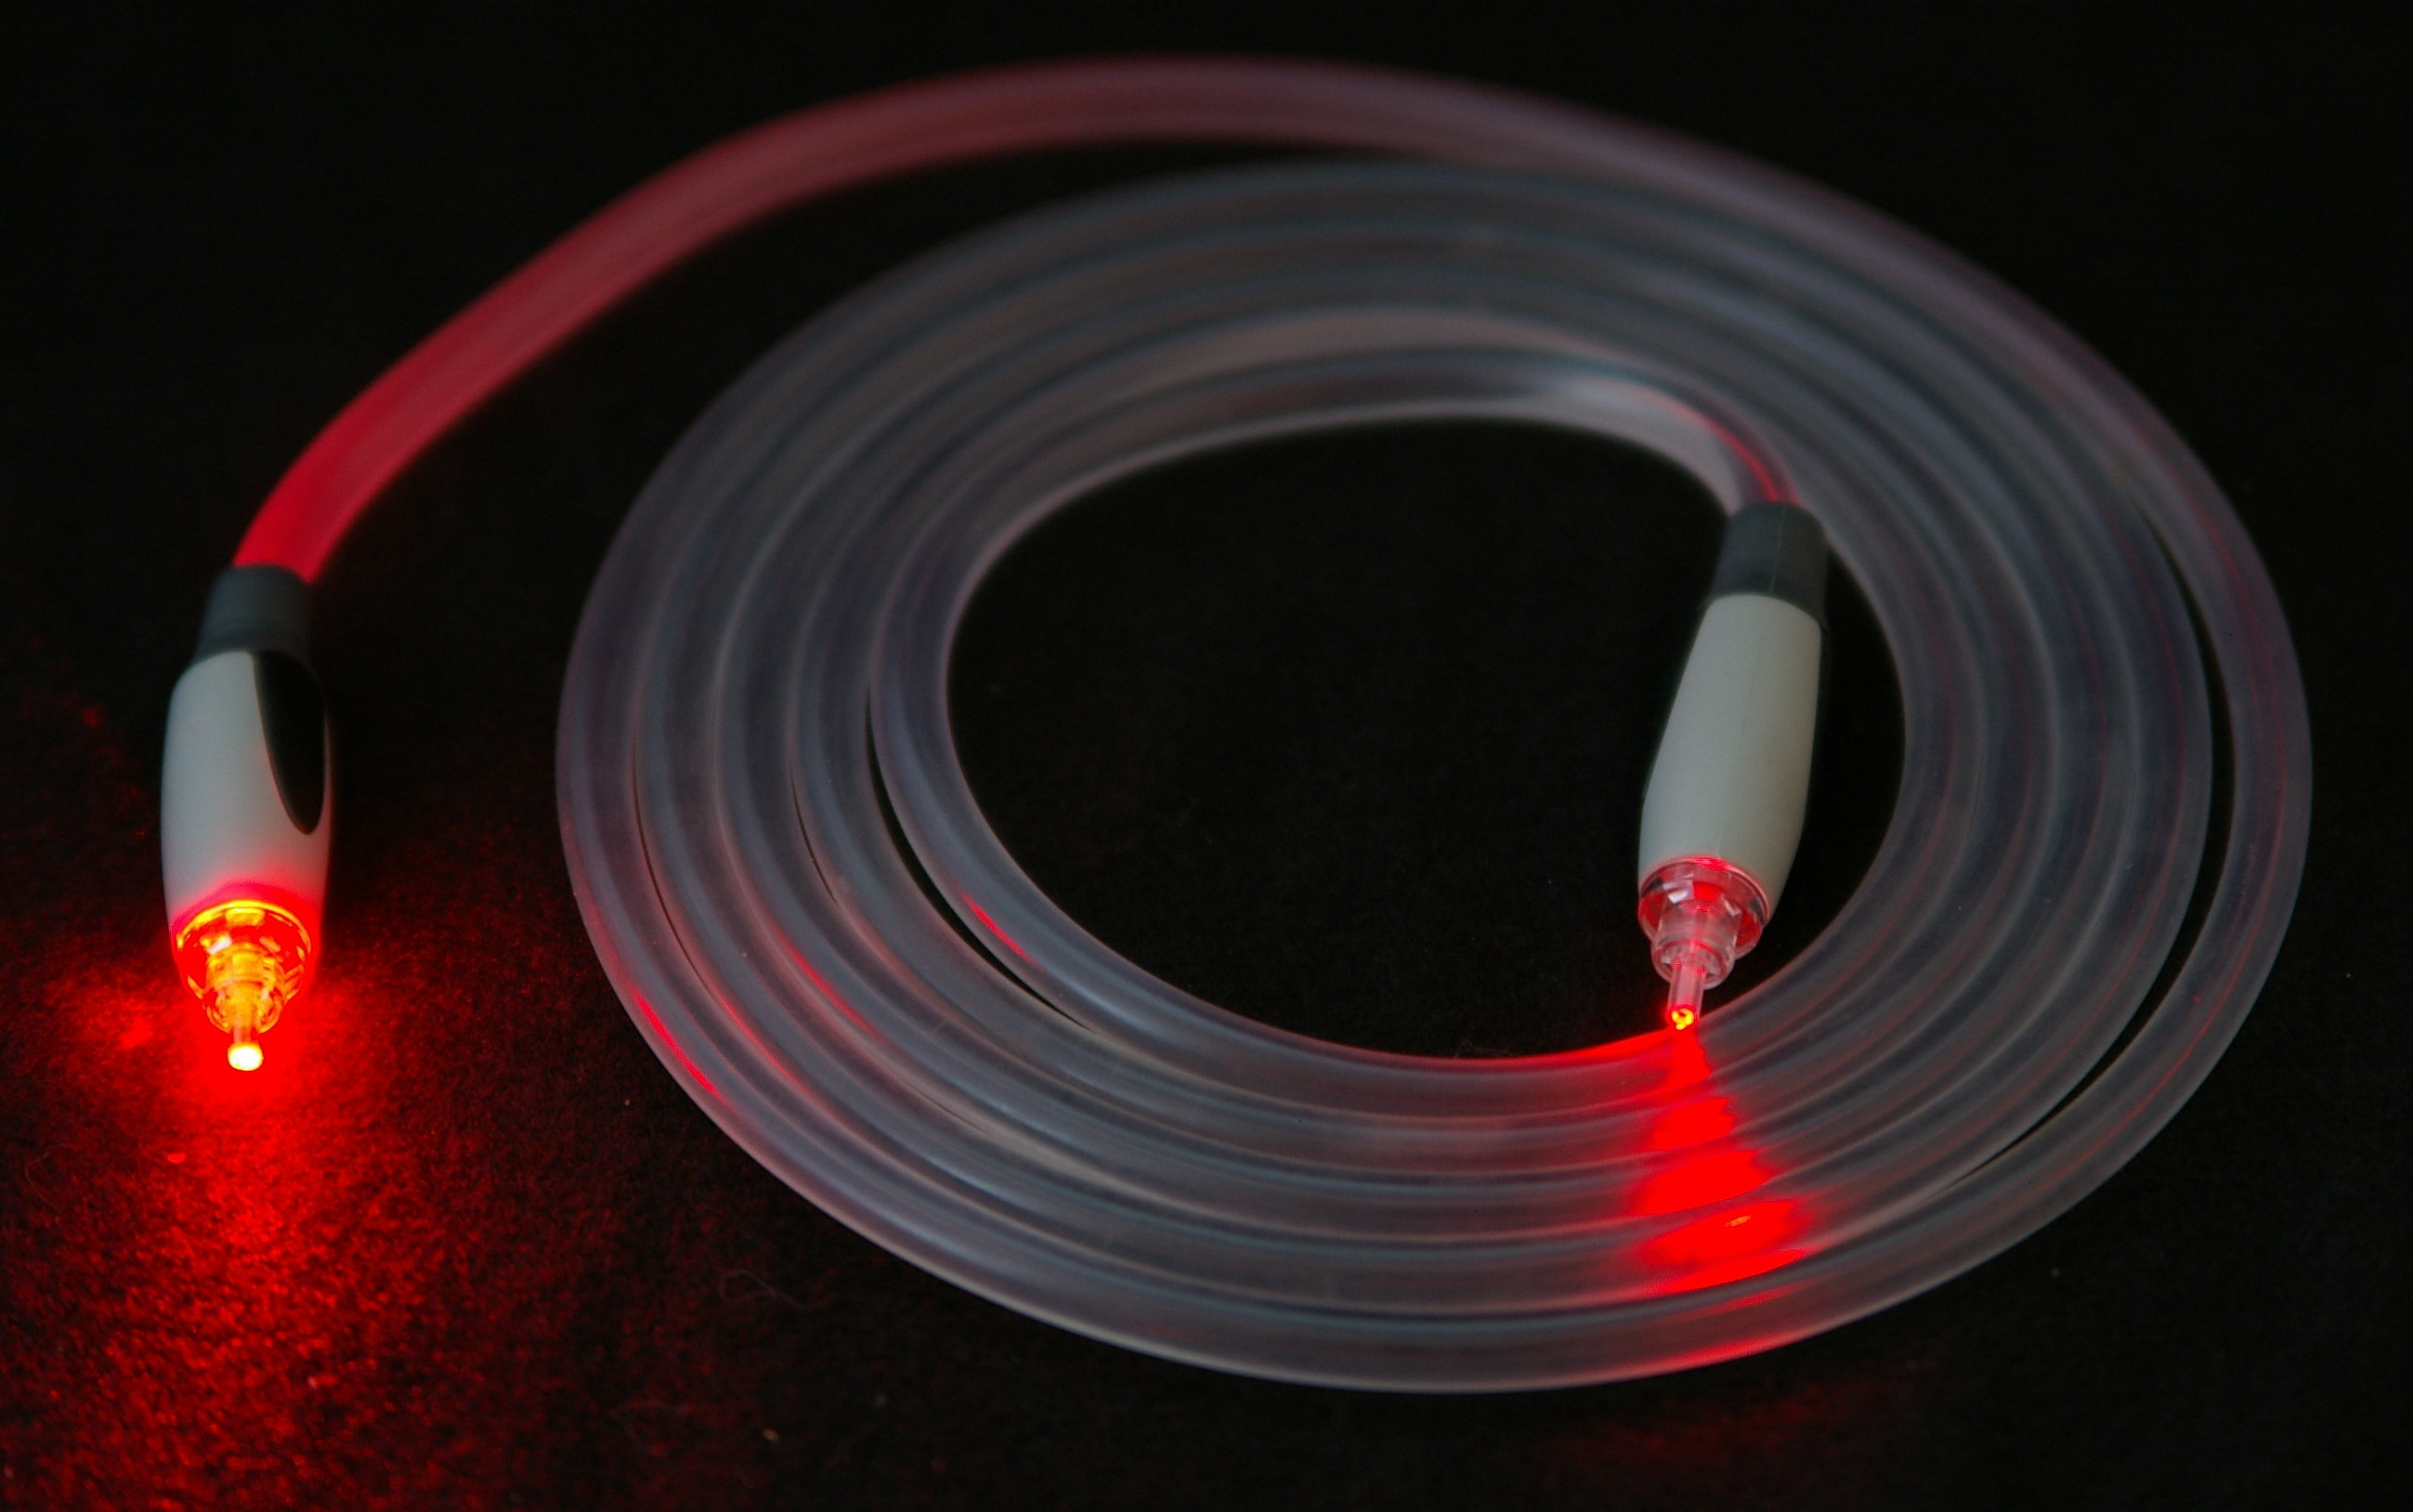
\includegraphics[width=4.3cm]{../physical/Fiber_optic_illuminated.jpeg}
}; \&
\node[draw,label={[credit]south:Dmitry G, CC BY-SA 3.0, via Wikimedia Commons},
      label={[type]north:bundle of wires}] (eth)  {
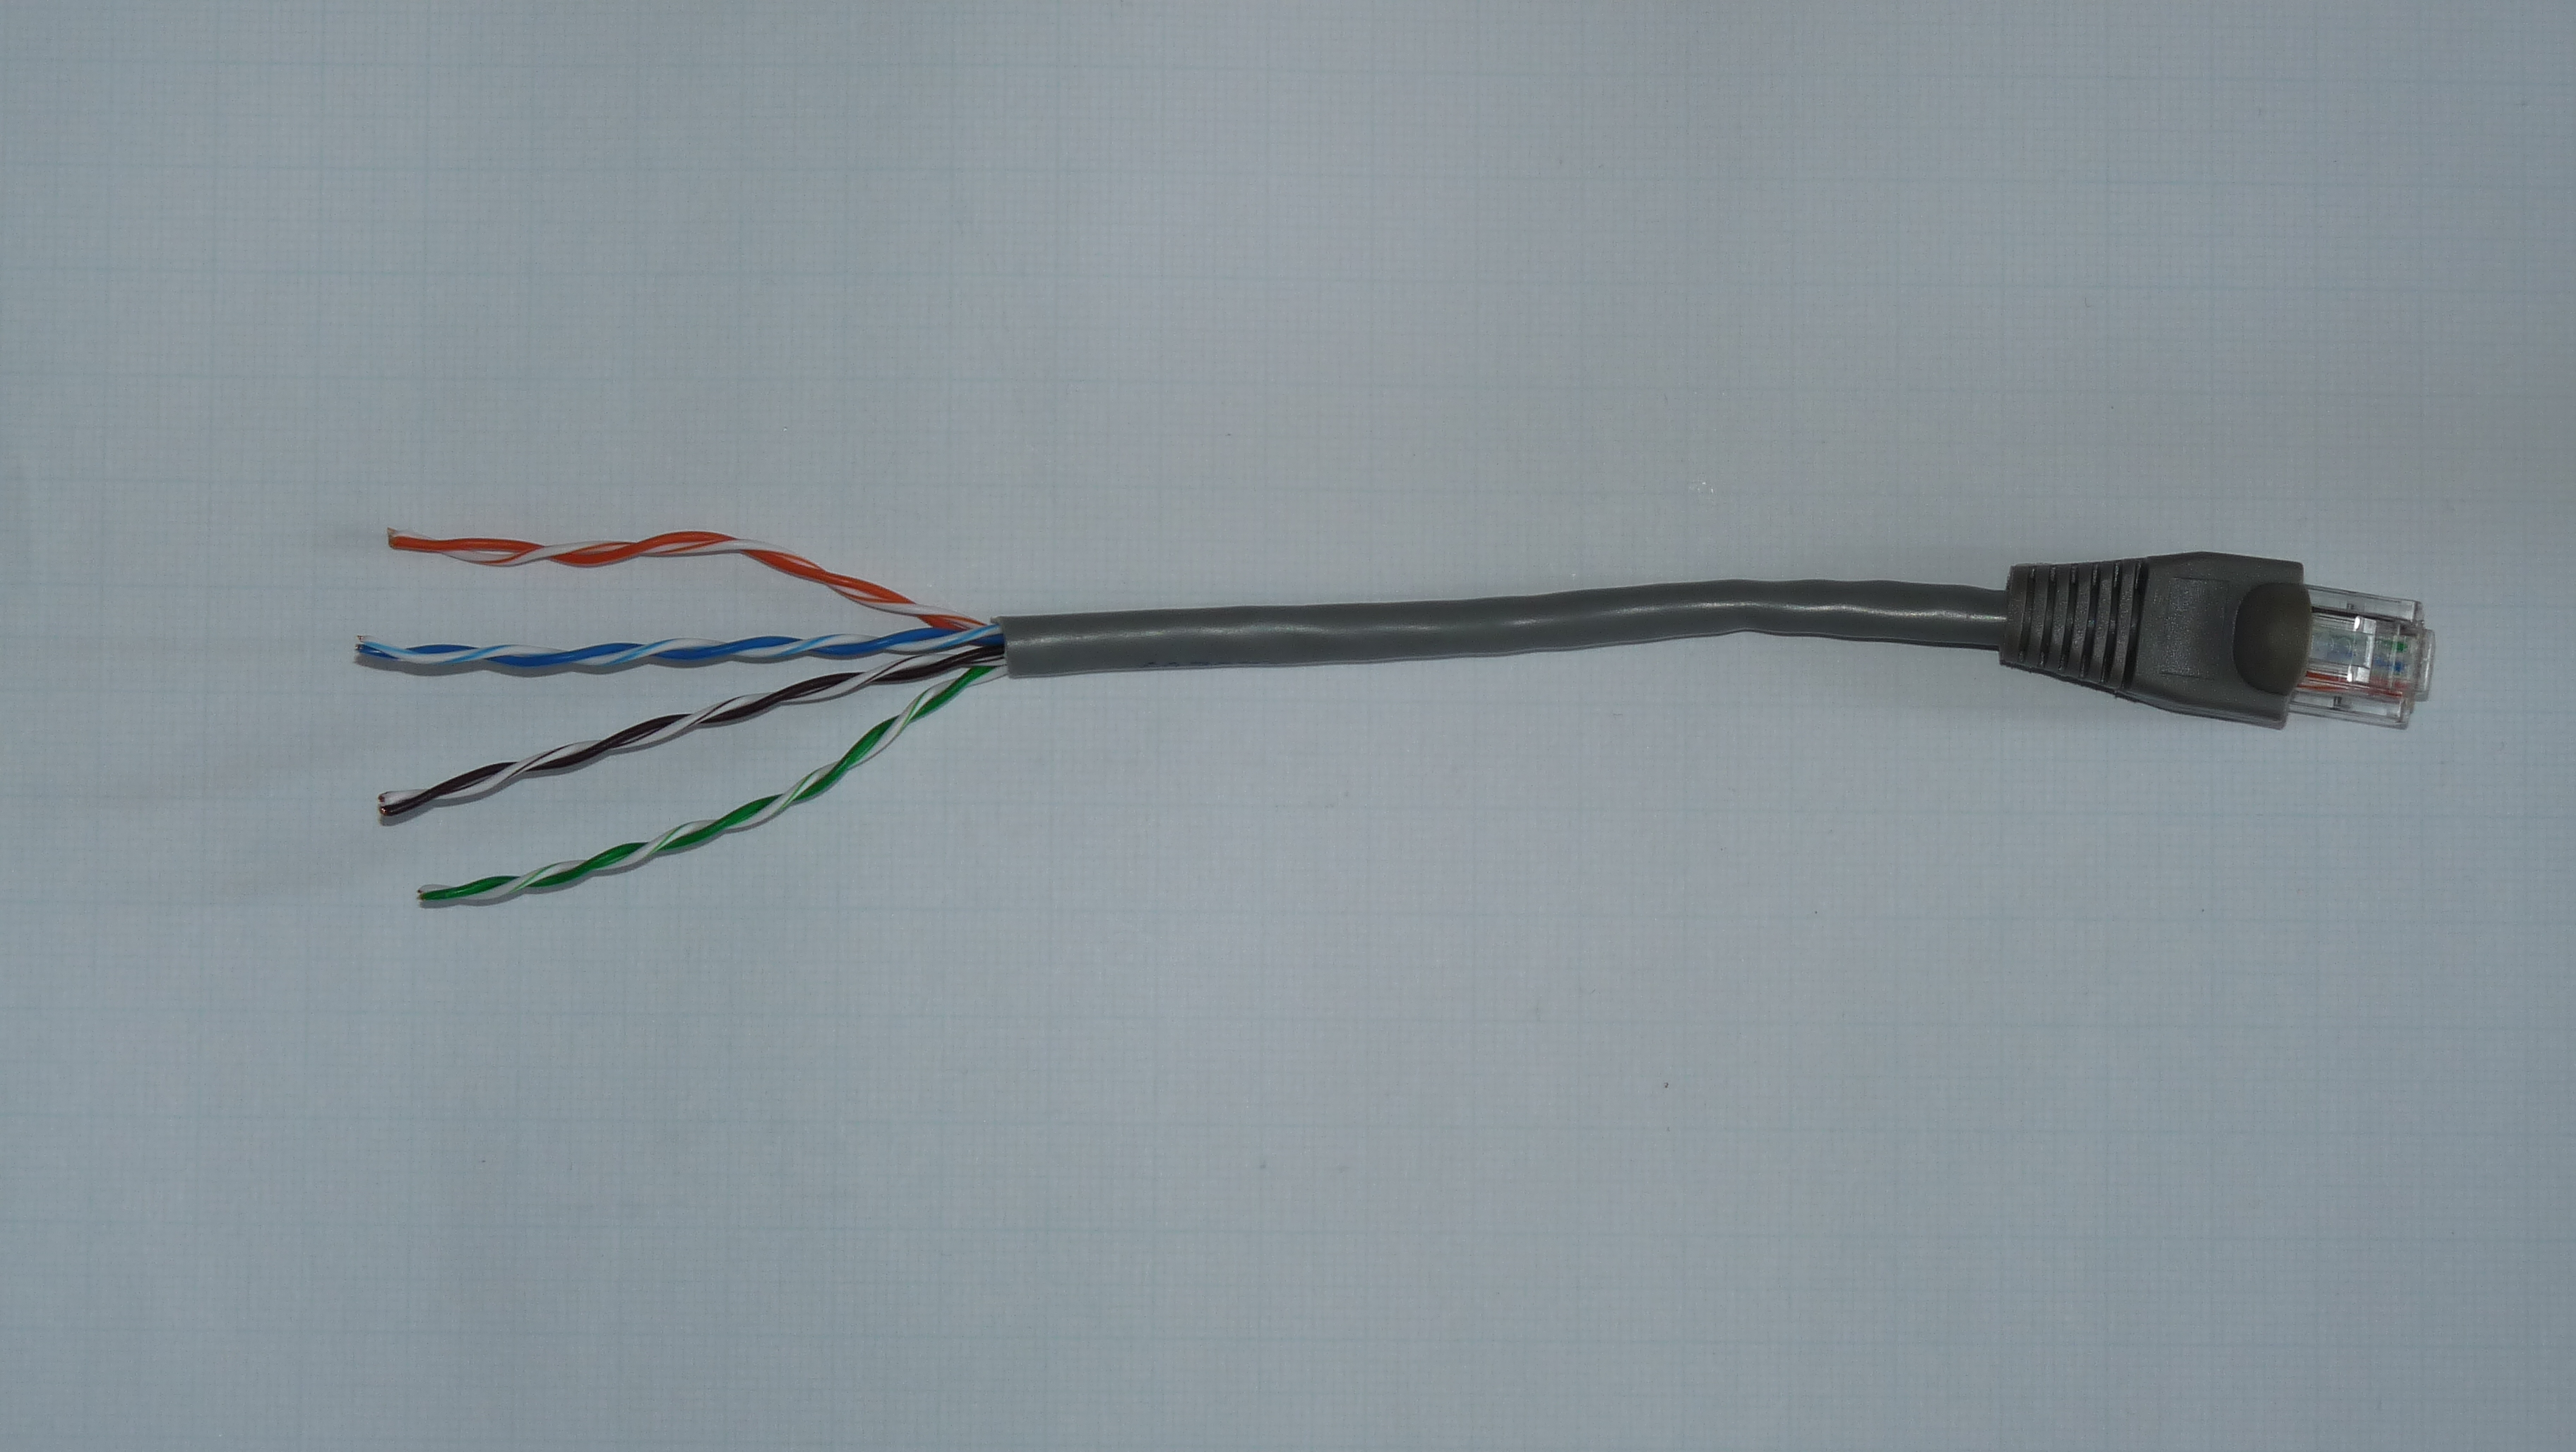
\includegraphics[width=4.3cm]{../physical/Ethernet_cable.jpeg}
}; \&
\node[draw,label={[credit]south:Adamantios, CC BY-SA 3.0, via Wikimedia Commons},
      label={[type]north:infrared through air}] (fso)  {
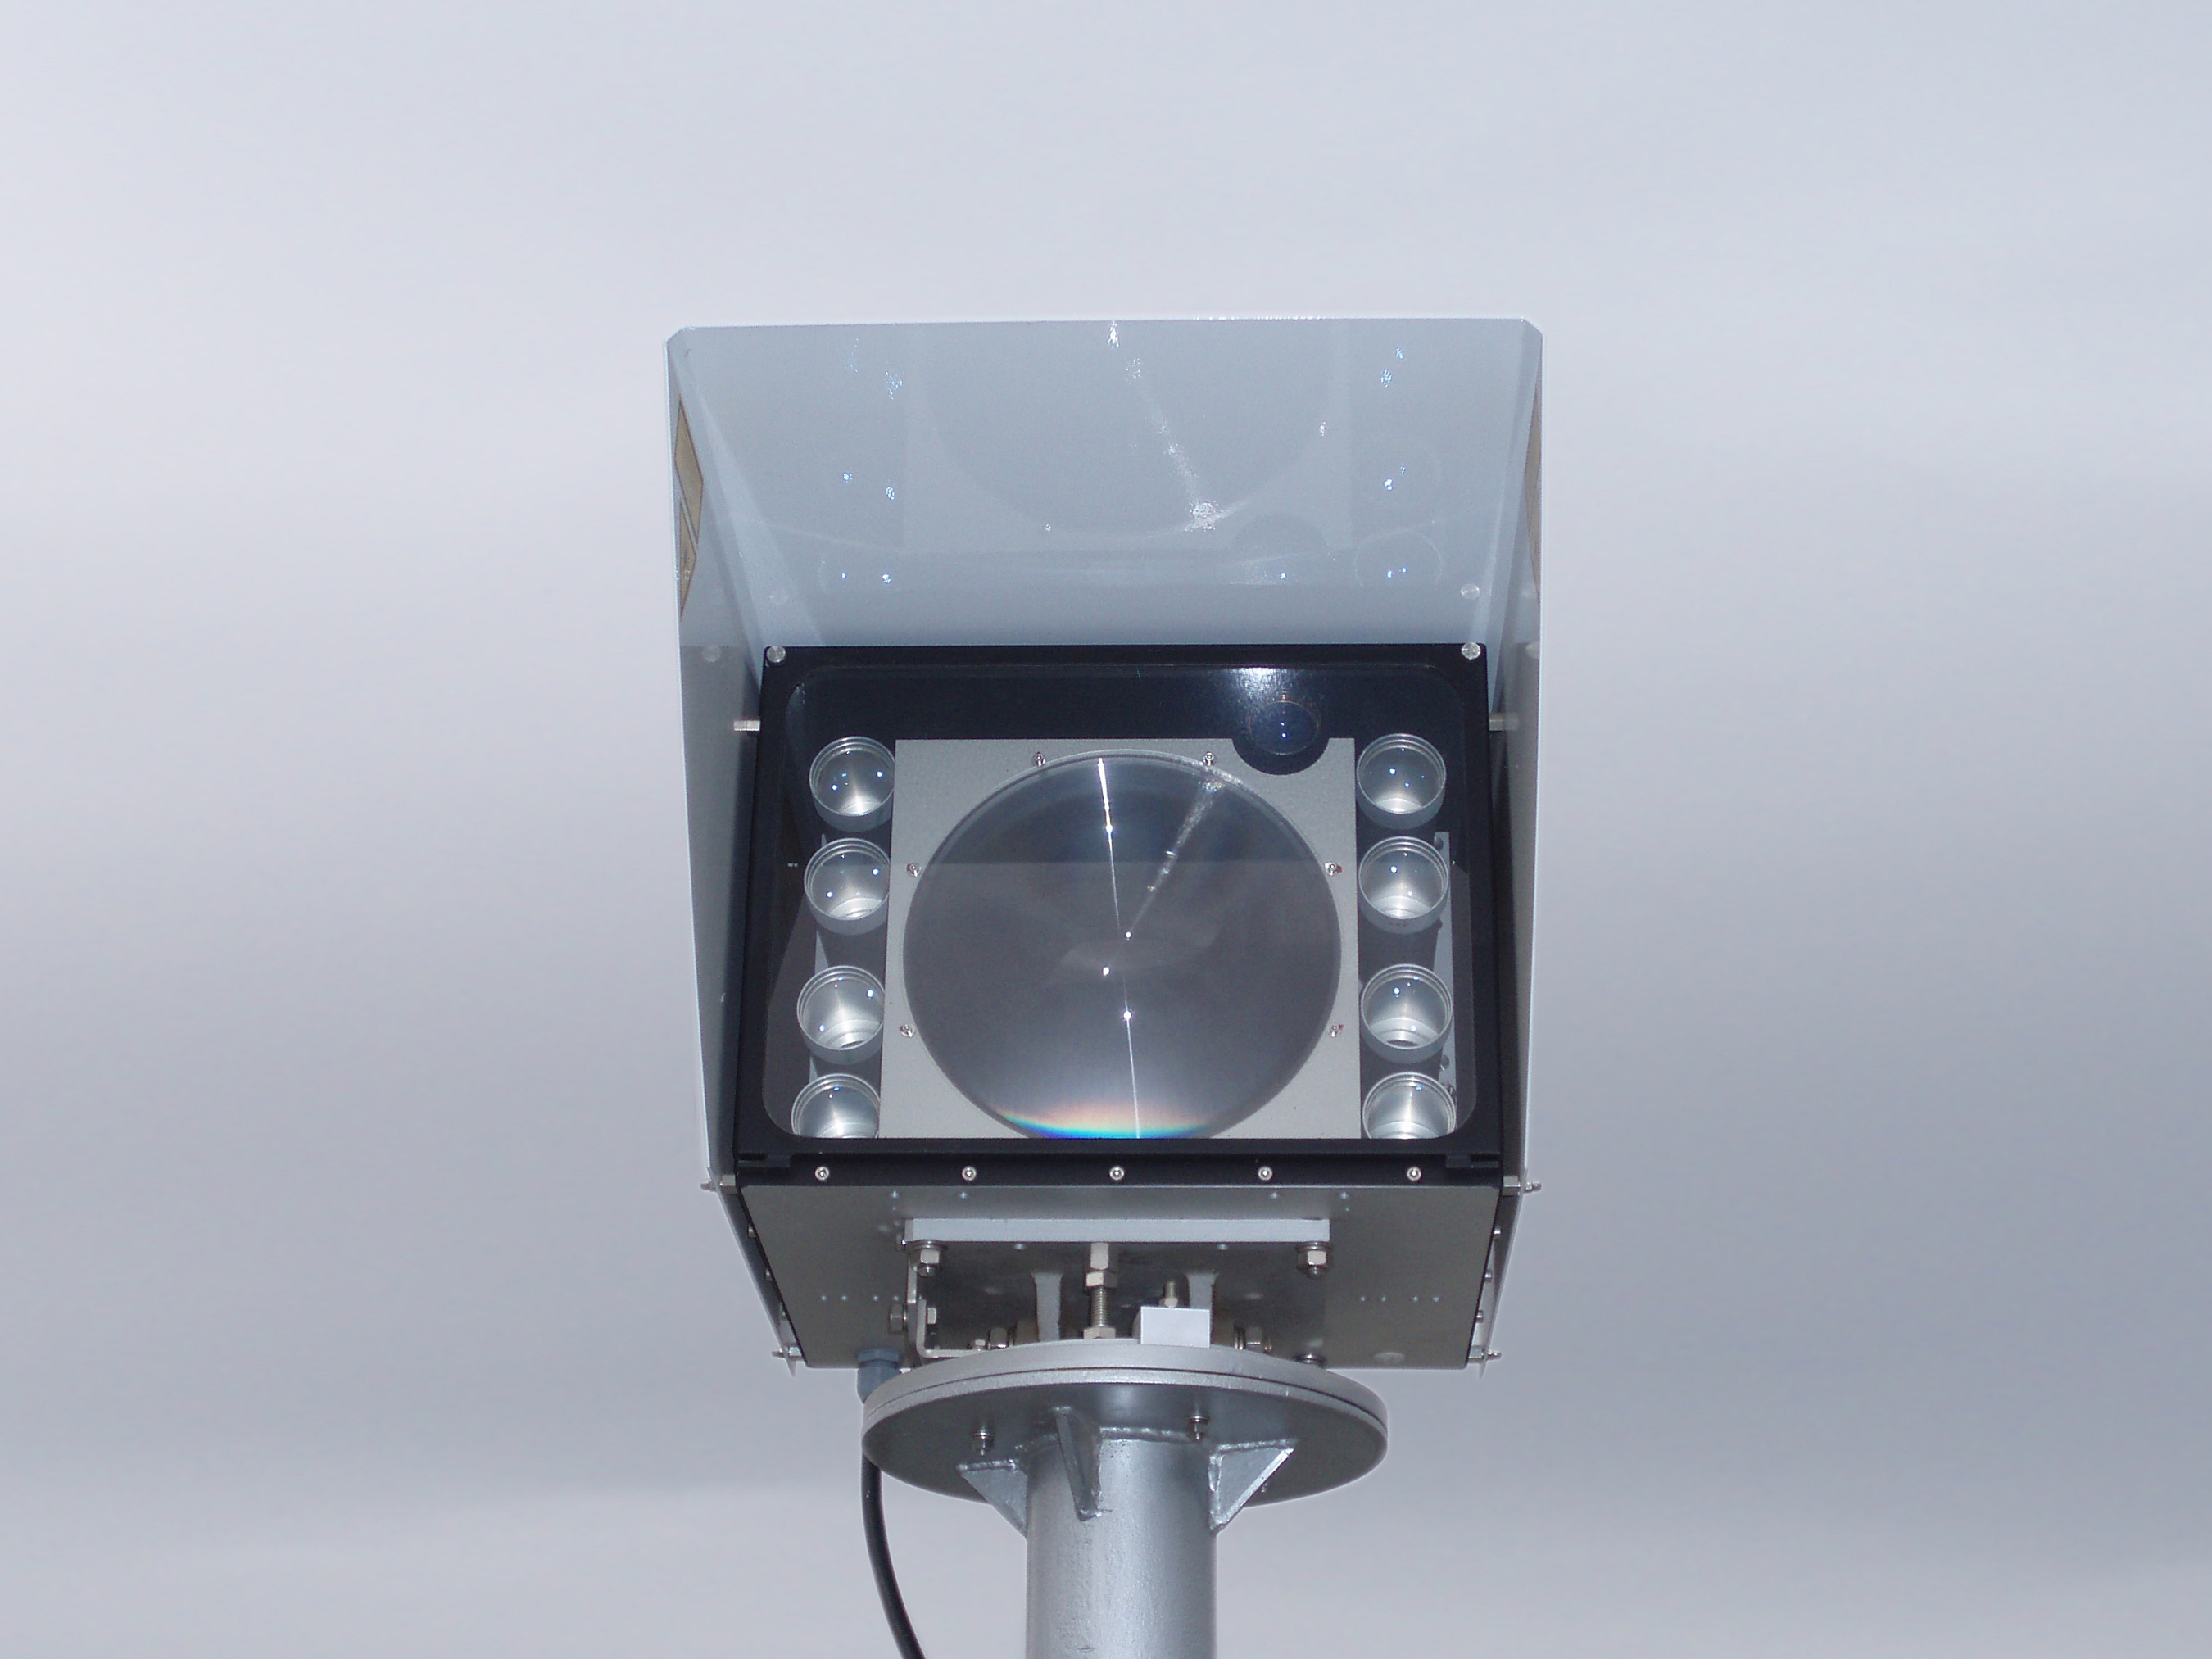
\includegraphics[width=3.7cm]{../physical/FSO-gigabit-laser-link-0a.jpeg}
}; \\
\node[draw,label={[credit]south:FDominec, CC BY-SA 3.0, via Wikimedia Commons},
      label={[type]north:single wire}] (coax)  {
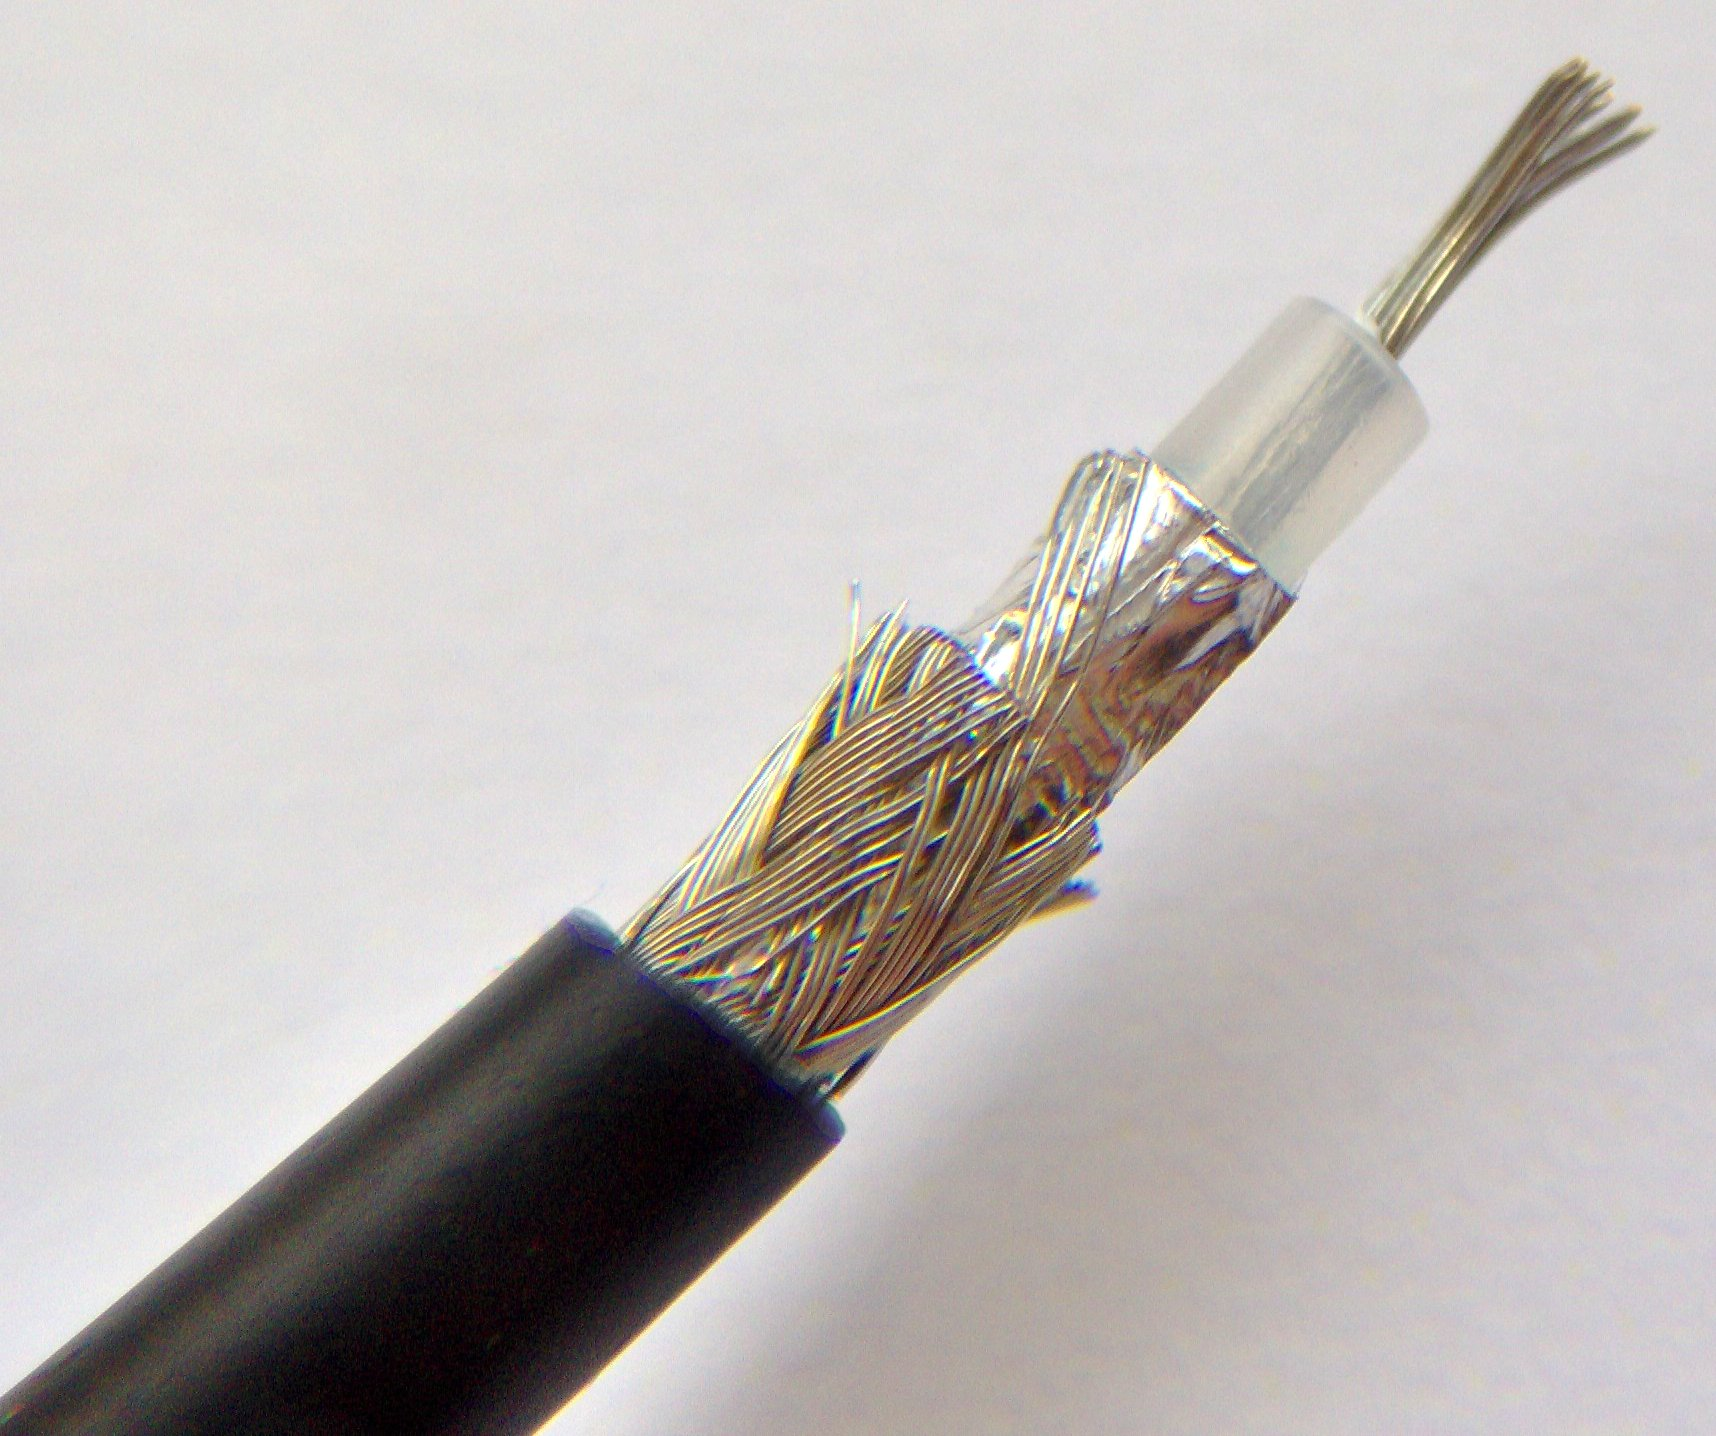
\includegraphics[width=3.3cm]{../physical/Coaxial_cable_cut.jpeg}
}; \&
\node[draw,label={[credit]south:Evan-Amos, via Wikimedia Commons},
      label={[type]north:radio}] (wifi)  {
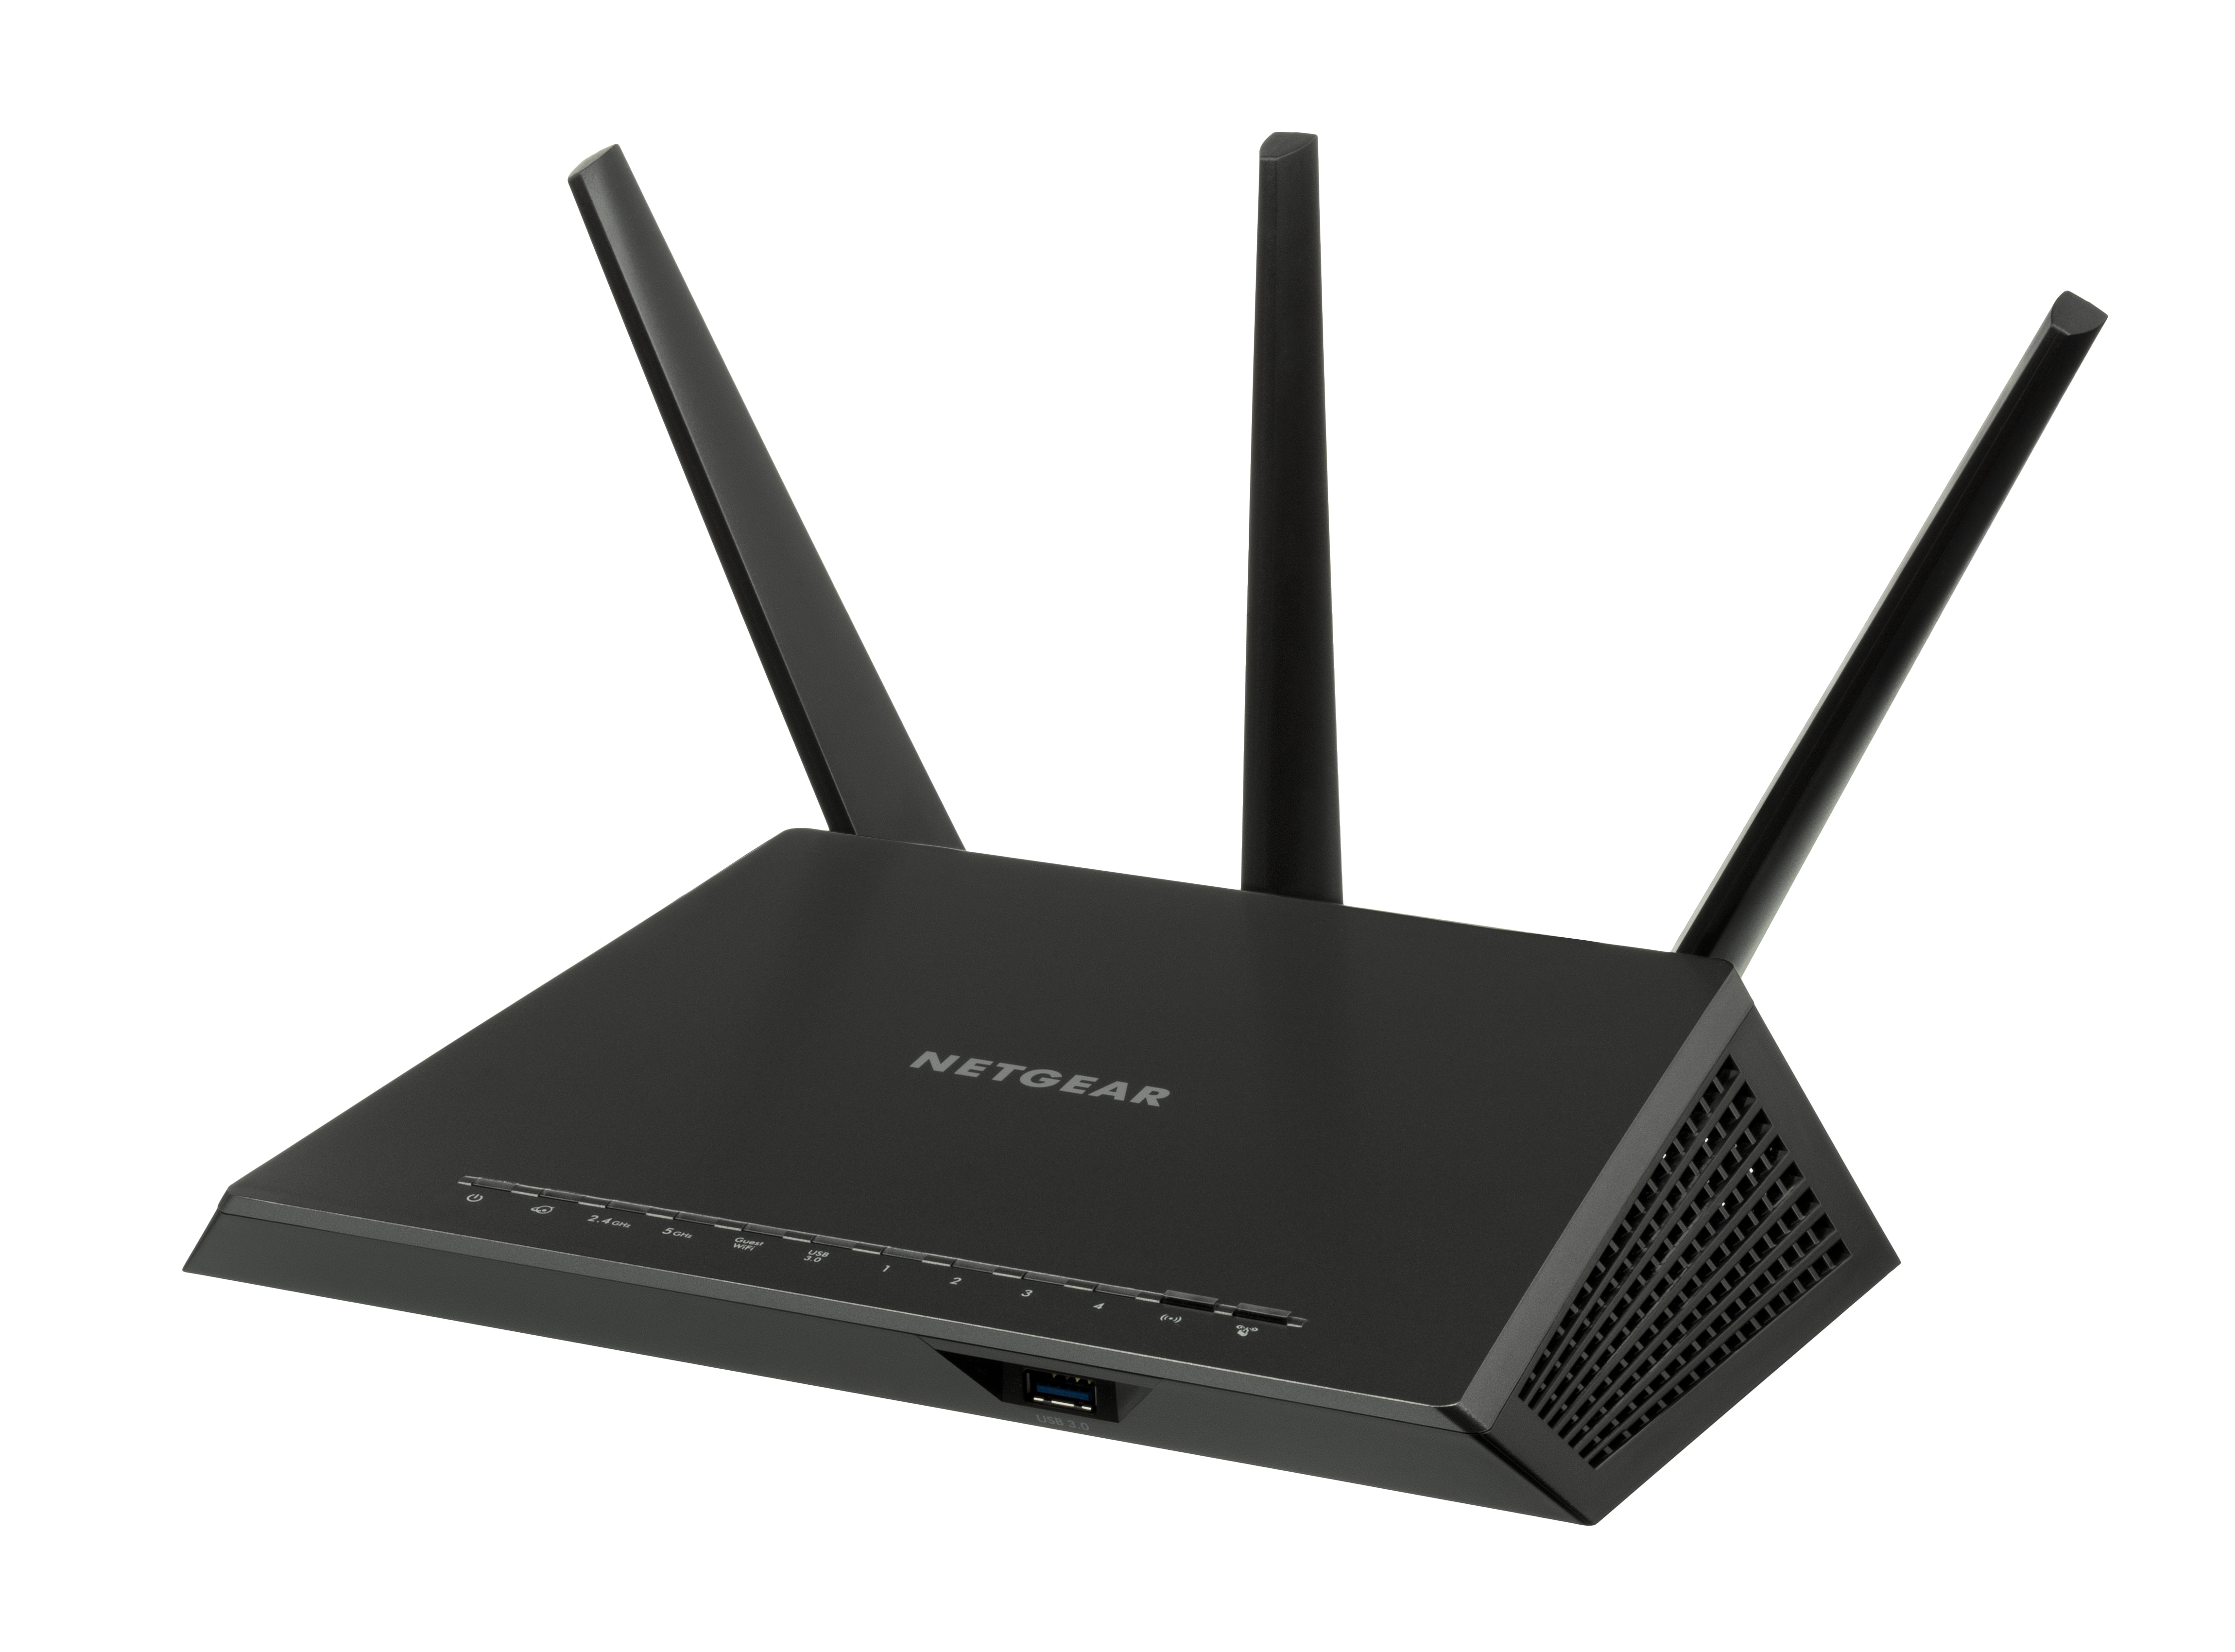
\includegraphics[width=3.7cm]{../physical/Netgear-Nighthawk-AC1900-WiFi-Router.jpeg}
}; \& \node[draw=none] (dotdot place) {}; \\
};
\node[draw=none,font=\Huge,anchor=center] (dotdot) at (wifi.east -| dotdot place.center){\ldots};
\end{tikzpicture}
\end{frame}


\subsection{transmitting a signal}
\usetikzlibrary{arrows.meta,calc,fadings,patterns}
\begin{frame}{transmitting a signal}
    \begin{itemize}
    \item can vary\ldots
        \begin{itemize}
        \item voltage
        \item radio/light intensity 
        \item radio/light frequency
        \item \ldots
        \end{itemize}
    \end{itemize}
\begin{tikzpicture}
\tikzset{
    axis/.style={draw,ultra thick,-Latex},
    signal/.style={draw,very thick,violet},
    axis label/.style={draw,thin,font=\small},
},
\begin{pgfonlayer}{fg}
    \draw[axis] (0, 0) -- (0, 3);
    \draw[axis] (0, 0) -- (14, 0);
\end{pgfonlayer}
\draw[axis label] (0, .3) -- ++ (-.2, 0) node[left] {low};
\draw[axis label] (0, 2.1) -- ++ (-.2, 0) node[left] {high};
\begin{scope}
    \clip (0, 0) rectangle (14, 3);
    %\begin{scope}[yshift=.3cm,y=1.8cm]
    %\draw[signal] (0, 0) -- (3, 0) -- (3, 1) -- (5, 1) -- (5, 0) -- (9, 0) -- (9, 1) -- (11, 1) -- (11, 0) -- (16, 0);
    %\end{scope}
    \begin{scope}[yshift=.3cm,y=0.6cm]
    \draw[signal] (0, 0) -- (3, 0) -- (3, 1) -- (5, 1) -- (5, 3) -- (9, 3) -- (9, 1) -- (11, 1) -- (11, 2) --
        (13, 2) -- (13, 0) -- (15, 0);
    \end{scope}
    \fill[white,path fading=west] (12, 0) rectangle (13.8, 3);
    \fill[white] (13.8, 0) rectangle (14, 3);
\end{scope}
\end{tikzpicture}
\end{frame}

\begin{frame}{some simplifying assumptions}
    \begin{itemize}
    \item signal low/high --- no in between
    \item only one `channel' 
        \begin{itemize}
        \item won't have multiple wires/antennas/frequencies/etc.
        \item won't modulate different things same time
        \end{itemize}
    \item want to send receive bits (0 or 1)
    \end{itemize}
\begin{tikzpicture}
\tikzset{
    axis/.style={draw,ultra thick,-Latex},
    signal/.style={draw,very thick,violet},
    axis label/.style={draw,thin,font=\small},
},
\begin{pgfonlayer}{fg}
    \draw[axis] (0, 0) -- (0, 3);
    \draw[axis] (0, 0) -- (14, 0);
\end{pgfonlayer}
\draw[axis label] (0, .3) -- ++ (-.2, 0) node[left] {low};
\draw[axis label] (0, 2.1) -- ++ (-.2, 0) node[left] {high};
\begin{scope}
    \clip (0, 0) rectangle (14, 3);
    \begin{scope}[yshift=.3cm,y=1.8cm]
    \draw[signal] (0, 0) -- (3, 0) -- (3, 1) -- (5, 1) -- (5, 0) -- (9, 0) -- (9, 1) -- (11, 1) -- (11, 0) -- (16, 0);
    \end{scope}
    \fill[white,path fading=west] (12, 0) rectangle (13.8, 3);
    \fill[white] (13.8, 0) rectangle (14, 3);
\end{scope}
\end{tikzpicture}
\end{frame}

\begin{frame}{clocking}
\begin{tikzpicture}
\tikzset{
    axis/.style={draw,ultra thick,-Latex},
    signal/.style={draw,very thick,violet},
    axis label/.style={draw,thin,font=\small},
    value/.style={font=\tt},
},
\begin{pgfonlayer}{fg}
    \draw[axis] (0, 0) -- (0, 3);
    \draw[axis] (0, 0) -- (14, 0);
\end{pgfonlayer}
\draw[axis label] (0, .3) -- ++ (-.2, 0) node[left] {low};
\draw[axis label] (0, 2.1) -- ++ (-.2, 0) node[left] {high};
\begin{scope}
    \clip (0, 0) rectangle (14, 3);
    \begin{scope}[yshift=.3cm,y=1.8cm]
    \draw[signal] (0, 0) -- (2.85, 0) -- (2.85, 1) -- (5.05, 1) -- (5.05, 0) -- (9.05, 0) -- (9.05, 1) -- (11.1, 1) -- (11.1, 0) -- (16, 0);
    \end{scope}
    \fill[white,path fading=west] (12, 0) rectangle (13.8, 3);
    \fill[white] (13.8, 0) rectangle (14, 3);
\end{scope}
\begin{visibleenv}<2,5>
\begin{scope}[yshift=-.8cm,xshift=1cm,x=2cm]
\foreach \x/\v in {0/0,1/1,2/0,3/0,4/1,5/0,6/0} {
    \draw[thick,dotted] (\x, -0.5) -- ++(0, 4.5cm);
    \node[value,anchor=north] at (\x+0.5, 0) {\v};
}
\end{scope}
\end{visibleenv}
\begin{visibleenv}<4,5>
\begin{scope}
\clip[overlay] (0, -10) rectangle (15, 10);
\begin{scope}[yshift=-.2cm,xshift=1.35cm,x=1.6cm]
\foreach \x/\v in {-1/0,0/0,1/1,2/0,3/0,4/0,5/1,6/0,7/0,8/0} {
    \draw[thick,dashed] (\x, -.5) -- ++(0, 4cm);
    \node[value,anchor=north] at (\x+0.5, 0) {\v};
}
\end{scope}
\end{scope}
\end{visibleenv}
\begin{visibleenv}<3,5>
\begin{scope}[yshift=-1.3cm,xshift=1cm,x=1cm]
\foreach \x/\v in {0/0,1/0,2/1,3/1,4/0,5/0,6/0,7/0,8/1,9/1,10/0,11/0} {
    \draw[thick,dashed] (\x, -.5) -- ++(0, 5cm);
    \node[value,anchor=north] at (\x+0.5, 0) {\v};
}
\end{scope}
\end{visibleenv}
\end{tikzpicture}
\end{frame}

\begin{frame}{keeping a clock}
\begin{tikzpicture}
\tikzset{
    axis/.style={draw,ultra thick,-Latex},
    signal/.style={draw,very thick,violet},
    axis label/.style={draw,thin,font=\small},
    value/.style={font=\tt},
},
\begin{pgfonlayer}{fg}
    \draw[axis] (0, 0) -- (0, 3);
    \draw[axis] (0, 0) -- (14, 0);
\end{pgfonlayer}
\draw[axis label] (0, .3) -- ++ (-.2, 0) node[left] {low};
\draw[axis label] (0, 2.1) -- ++ (-.2, 0) node[left] {high};
\begin{scope}
    \clip (0, 0) rectangle (14, 3);
    \begin{scope}[yshift=.3cm,y=1.8cm]
    \draw[signal] (0, 0) -- (2.85, 0) -- (2.85, 1) -- (5.05, 1) -- (5.05, 0) -- (9.05, 0) -- (9.05, 1) -- (11.1, 1) -- (11.1, 0) -- (16, 0);
    \end{scope}
    \fill[white,path fading=west] (12, 0) rectangle (13.8, 3);
    \fill[white] (13.8, 0) rectangle (14, 3);
\end{scope}

\begin{scope}[yshift=-4cm]
    \begin{pgfonlayer}{fg}
        \draw[axis] (0, 0) -- (0, 3);
        \draw[axis] (0, 0) -- (14, 0);
    \end{pgfonlayer}
    \draw[axis label] (0, .3) -- ++ (-.2, 0) node[left] {low};
    \draw[axis label] (0, 2.1) -- ++ (-.2, 0) node[left] {high};
    \begin{scope}
        \clip (0, 0) rectangle (14, 3);
        \begin{scope}[yshift=.3cm,y=1.8cm]
        \begin{visibleenv}<2->
        \draw[signal,alt=<3->{opacity=0.1}]
            (0, 1) -- (1, 1) -- (1, 0) -- (2, 0) -- (2, 1) 
        -- (2.95, 1) -- (2.95, 0) -- (4, 0) -- (4, 1) -- (5.08, 1) -- (5.08, 0)
        -- (6, 0) -- (6, 1) -- (7.05, 1) -- (7.05, 0) -- (8, 0) -- (8, 1)
        -- (8.95, 1) -- (8.95, 0) -- (10, 0) -- (10, 1) -- (11.0, 1) -- (11.0, 0)
        -- (12, 0) -- (12, 1) -- (13, 1) -- (13, 0) -- (14, 0) -- (14, 1) --(15, 1);
        \end{visibleenv}
        \begin{visibleenv}<3-4>
        \draw[signal]
            (0, 1) -- (1, 1) -- (1, 0) -- (2, 0) -- (2, 1) 
        -- (2.85, 1) edge[red] (2.85, 0) (2.85,0) -- (3.9, 0) edge[red] (3.9, 1) (3.9, 1)-- (5.05, 1) edge[red] (5.05, 0)
        (5.05, 0)
        -- (6, 0) -- (6, 1) -- (7.05, 1) -- (7.05, 0) -- (8, 0) -- (8, 1)
        -- (9.05, 1) edge[red] (9.05, 0) (9.05, 0) -- (10.05, 0) edge[red] (10.05, 1) (10.05, 1) -- (11.1, 1) edge[red] (11.1, 0) (11.0, 0)
        -- (12, 0) -- (12, 1) -- (13.1, 1) edge[red] (13.1, 0) (13.1, 0) -- (14, 0) -- (14, 1) --(15, 1);
        \end{visibleenv}
        \end{scope}
        \fill[white,path fading=west] (12, 0) rectangle (13.8, 3);
        \fill[white] (13.8, 0) rectangle (14, 3);
    \end{scope}
\end{scope}
\begin{visibleenv}<2->
    \begin{scope}[yshift=-.2cm,xshift=1cm,x=2cm]
    \foreach \x/\v in {0/0,1/1,2/0,3/0,4/1,5/0,6/0} {
        \node[value,anchor=north] at (\x+0.5, 0) {\v};
    }
    \end{scope}
    \begin{scope}[yshift=-.2cm]
    \foreach \loc in {1,2.95,5.08,7.05,8.95,11,13,15} {
        \draw[thick,dashed] (\loc, -4) -- ++(0, 7);
    }
    \end{scope}
\end{visibleenv}
\begin{visibleenv}<3-4>
    \begin{scope}[yshift=-.2cm]
    \tikzset{
        marked/.style={red,ultra thick},
    }
    \foreach \loc/\mark in {1/,2.85/marked,5.05/marked,7.05/,9.05/marked,11.1/marked,13.1/marked,15.1/} {
        \draw[thick,dashed,\mark] (\loc, -4) -- ++(0, 7);
    }
    \end{scope}
\end{visibleenv}
\end{tikzpicture}
\end{frame}

\begin{frame}{self-synchronizing?}
    \begin{itemize}
    \item can resynchronize clock by looking for transitions
    \item but doesn't work if lots of consecutive 0s or 1s
    \vspace{.5cm}
    \item also, need to know where low and high point is
    \item important to have transitions to low/high to calibrate this
    \end{itemize}
\end{frame}

\begin{frame}{Manchester encoding}
\begin{tikzpicture}
\node (fig) { 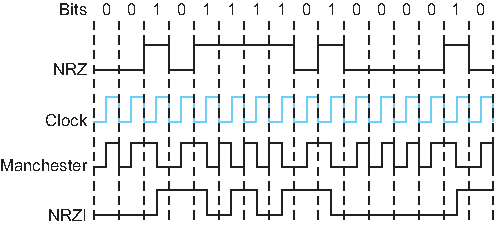
\includegraphics[width=0.9\textwidth]{../physical/SysApproach-2-Fig-25.pdf} };
\end{tikzpicture}
\imagecredit{Figure 25 from Section 2.2 of \textit{Computer Networks: A Systems Approach} (6th ed) (Peterson and Davie)}
\end{frame}

\begin{frame}{problem with Manchester}
    \begin{itemize}
    \item fixed the problem of too few transitions
    \vspace{.5cm}
    \item but now most transitions don't send information
    \item means we aren't making goo duse of wire/etc. capacity
    \vspace{.5cm}
    \item there are more clever compromises
        \begin{itemize}
        \item (example: 4B5B encoding)
    \end{itemize}
\end{frame}

\begin{frame}{other better encoding options}
    \begin{itemize}
    \item vary more than just one thing
        \begin{itemize}
        \item example: pulse amplitude and duration
        \end{itemize}
    \item use more than just low/high
    \item \ldots much more
    \vspace{.5cm}
    \item probably covered in ECE Signals course?
    \end{itemize}
\end{frame}


\subsection{synchronizing (short)}


\begin{frame}{self-synchronizing?}
    \begin{itemize}
    \item can resynchronize clock by looking for transitions
    \item but doesn't work if lots of consecutive 0s or 1s
    \vspace{.5cm}
    \item also, need to know where low and high point is
    \item important to have transitions to low/high to calibrate this
    \end{itemize}
\end{frame}

\begin{frame}{self-sync and `start-message'}
    \begin{itemize}
    \item one idea: set start-message to have lots of 0/1/0/1/0/1/0/1/etc.
        \begin{itemize}
        \item something 10Mbit Ethernet does
        \end{itemize}
    \item but probably not enough to ensure things stay in sync on big message
    \vspace{.5cm}
    \item alternate strategy --- use encoding that adds extra transitions
    \item example: Manchester encoding
    \end{itemize}
\end{frame}


\subsectoin{better options?}
\begin{frame}{other better encoding options}
    \begin{itemize}
    \item vary more than just one thing
        \begin{itemize}
        \item example: pulse amplitude and duration
        \end{itemize}
    \item use more than just low/high
    \item \ldots much more
    \vspace{.5cm}
    \item probably covered in ECE Signals course?
    \end{itemize}
\end{frame}




\section{simple reliablity}

\subsection{adding acknowledgments}
\usetikzlibrary{arrows.meta,shapes.misc,decorations.pathreplacing}

\begin{frame}{dealing with network message lost}
\begin{tikzpicture}
\tikzset{
    box/.style={draw,thick,minimum width=2cm},
    message/.style={draw,thick,-Latex},
    failure/.style={draw,ultra thick,red,cross out,minimum width=1cm,minimum height=1cm},
}
\begin{scope}
\draw[box] (0, 0) rectangle ++(2, -3) 
    node[midway,align=center] {machine\\ A};
\draw[box] (13, 0) rectangle ++(2, -3) 
    node[midway,align=center] {machine\\B};
\draw[message] (2, -1) -- (13, -2) node[pos=0.35, above, sloped] {``The meeting is at 12pm.''};
\end{scope}
\draw[ultra thick] (0, -3.5) -- ++ (13,0);
\begin{scope}[yshift=-4cm]
\draw[box] (0, 0) rectangle ++(2, -3) 
    node[midway,align=center] {machine\\A};
\draw[box] (13, 0) rectangle ++(2, -3) 
    node[midway,align=center] {machine\\B};
\draw[message] (2, -1) -- (9, -1.5) 
    node[pos=0.5,above,sloped] {``The meeting is at 12pm.''}
    node[failure] {};
\end{scope}
\end{tikzpicture}
\end{frame}

\begin{frame}{handling lost message: acknowledgements}
\begin{tikzpicture}
\tikzset{
    box/.style={thick},
    message/.style={draw,thick,-Latex},
    failure/.style={draw,ultra thick,red,cross out,minimum width=1cm,minimum height=1cm},
}
\begin{scope}
\draw[box] (0, 0) rectangle ++(2, -8) 
    node[midway,align=center] {machine\\A};
\draw[box] (13, 0) rectangle ++(2, -8) 
    node[midway,align=center] {machine\\B};
\draw[message] (2, -0.5) -- (13, -1) node[pos=0.35, above, sloped] {``The meeting is at 12pm.''};
\draw[message] (13, -1.5) -- (2, -2) node[pos=0.25, sloped,below] {Got it!};
\end{scope}
\end{tikzpicture}
\end{frame}

\begin{frame}{handling lost message}
\begin{tikzpicture}
\tikzset{
    box/.style={thick},
    message/.style={draw,thick,-Latex},
    failure/.style={draw,ultra thick,red,cross out,minimum width=1cm,minimum height=1cm},
}
\draw[box] (0, 0) rectangle ++(2, -8) 
    node[midway,align=center] {machine\\A};
\draw[box] (13, 0) rectangle ++(2, -8) 
    node[midway,align=center] {machine\\B};
%\draw[message] (2, -0.5) -- (13, -1) node[pos=0.35, above, sloped] {``The meeting is at 12pm.''};
\draw[message] (2, -0.5) -- (9, -1) 
    node[pos=0.5,above,sloped] {``The meeting is at 12pm.''}
    node[failure] {};
\begin{visibleenv}<2->
\draw[decorate,decoration={brace}] (2.1, -1) -- (2.1, -3) 
    node[midway,right,align=left] {
        ``timeout'' \\
        A doesn't get reply \\
        after waiting too long
    };
\end{visibleenv}
\begin{visibleenv}<3->
\draw[message] (2, -4) -- (13, -5) node[pos=0.35, above, sloped] {``The meeting is at 12pm.''};
\draw[message] (13, -5.5) -- (2, -6) node[pos=0.5, sloped,below] {Got it!};
\end{visibleenv}
\end{tikzpicture}
\end{frame}

\begin{frame}{protocol so far}
    \begin{itemize}
    \item on sender: until ACK received:
        \begin{itemize}
        \item (re)send frame of data
        \item wait fixed amount of time for ACK
        \end{itemize}
    \vspace{.5cm}
    \item on receiver: continuously:
        \begin{itemize}
        \item wait for frame of data
        \item send ACK back
        \end{itemize}
    \end{itemize}
\end{frame}


\subsection{sequence numbers}
\usetikzlibrary{arrows.meta,decorations.pathreplacing,shapes.misc}

\begin{frame}{problem}
    \begin{itemize}
    \item really want to send multiple frames
    \item example: data split in multiple pieces
    \end{itemize}
\end{frame}

\begin{frame}{splitting messages: try 1}
\begin{tikzpicture}
\tikzset{
    box/.style={thick},
    message/.style={draw,thick,-Latex},
    failure/.style={draw,ultra thick,red,cross out,minimum width=1cm,minimum height=1cm},
}
\begin{scope}
\draw[box] (0, 0) rectangle ++(2, -6) 
    node[midway,align=center] {machine\\A};
\draw[box] (13, 0) rectangle ++(2, -6) 
    node[midway,align=center] {machine\\B};
\draw[message] (2, -0.5) -- (13, -1) node[pos=0.25, above, sloped] {``The meeting''};
\draw[message] (13, -1.5) -- (2, -2) node[pos=0.25, sloped,below] {ACK};
\draw[message] (2, -2.5) -- (13, -3.5) node[pos=0.25, above, sloped] {`` is at 12pm.''};
\draw[message] (13, -4) -- (2, -4.5) node[pos=0.25, sloped,below] {ACK};
\end{scope}
\end{tikzpicture}
reconstructed message: \\
The meeting is at 12pm.
\end{frame}

\begin{frame}{splitting messages: try 1 --- problem 1}
\begin{tikzpicture}
\tikzset{
    box/.style={thick},
    message/.style={draw,thick,-Latex},
    failure/.style={draw,ultra thick,red,cross out,minimum width=1cm,minimum height=1cm},
}
\begin{scope}
\draw[box] (0, 0) rectangle ++(2, -6) 
    node[midway,align=center] {machine\\A};
\draw[box] (13, 0) rectangle ++(2, -6) 
    node[midway,align=center] {machine\\B};
\draw[message] (2, -0.5) -- (13, -0.75) node[pos=0.25, above, sloped] {``The meeting''};
\draw[message] (13, -1) -- (6, -1.5) node[pos=0.25, sloped,below] {ACK} node[failure] {};
\draw[message] (2, -2) -- (13, -2.5) node[pos=0.25, above, sloped] {``The meeting''};
\draw[message] (13, -3) -- (2, -3.5) node[pos=0.25, sloped,below] {ACK};
\draw[message] (2, -4) -- (13, -4.5) node[pos=0.25, above, sloped] {`` is at 12pm.''};
\draw[message] (13, -5) -- (2, -5.5) node[pos=0.25, sloped,below] {ACK};
\end{scope}
\end{tikzpicture}
\begin{visibleenv}<2->
reconstructed message: \\
The meetingThe meeting is at 12pm.
\end{visibleenv}
\end{frame}

\begin{frame}{exercise: other problems?}
\begin{itemize}
\item sending `The meeting', `is at 12pm'
\item what would be received for each of these scenarios?
\end{itemize}
\begin{tabular}{ll}
1. & message (instead of acknowledgment) is lost \\
2. & first message from machine A is delayed a long time by network \\
3. & acknowledgment of second message lost instead of first \\
\end{tabular}
\end{frame}

\begin{frame}{aside: message delays}
    \begin{itemize}
    \item long message delays not possible with direct link
    \vspace{.5cm}
    \item but are possible with:
        \begin{itemize}
        \item multiple paths from A to B
        \item doing this kind of acknowledgment + resending hop-by-hop
        \end{itemize}
    \end{itemize}
\end{frame}

\begin{frame}{splitting messages: try 2}
\begin{tikzpicture}
\tikzset{
    box/.style={thick},
    message/.style={draw,thick,-Latex},
    failure/.style={draw,ultra thick,red,cross out,minimum width=1cm,minimum height=1cm},
}
\begin{scope}
\draw[box] (0, 0) rectangle ++(2, -5) 
    node[midway,align=center] {machine\\A};
\draw[box] (13, 0) rectangle ++(2, -5) 
    node[midway,align=center] {machine\\B};
\draw[message] (2, -0.5) -- (13, -1) node[pos=0.25, above, sloped] {part 0: ``The meeting''};
\draw[message] (13, -1.5) -- (2, -2) node[pos=0.25, sloped,below] {ACK};
\draw[message] (2, -2.5) -- (13, -3) node[pos=0.25, above, sloped] {part 1: `` is at 12pm.''};
\draw[message] (13, -3.5) -- (2, -4) node[pos=0.25, sloped,below] {ACK};
\end{scope}
\end{tikzpicture}
reconstructed message: \\
The meeting is at 12pm.
\end{frame}

\begin{frame}{splitting messages: try 2 --- missed ack}
\begin{tikzpicture}
\tikzset{
    box/.style={thick},
    message/.style={draw,thick,-Latex},
    failure/.style={draw,ultra thick,red,cross out,minimum width=1cm,minimum height=1cm},
}
\begin{scope}
\draw[box] (0, 0) rectangle ++(2, -6) 
    node[midway,align=center] {machine\\A};
\draw[box] (13, 0) rectangle ++(2, -6) 
    node[midway,align=center] {machine\\B};
\draw[message] (2, -0.5) -- (13, -0.75) node[pos=0.25, above, sloped] {part 0: ``The meeting''};
\draw[message] (13, -1) -- (6, -1.5) node[pos=0.25, sloped,below] {ACK} node[failure] {};
\draw[message] (2, -2) -- (13, -2.5) node[pos=0.25, above, sloped] {part 0: ``The meeting''};
\draw[message] (13, -3) -- (2, -3.5) node[pos=0.25, sloped,below] {ACK};
\draw[message] (2, -4) -- (13, -4.5) node[pos=0.25, above, sloped] {part 1: `` is at 12pm.''};
\draw[message] (13, -5) -- (2, -5.5) node[pos=0.25, sloped,below] {ACK};
\end{scope}
\end{tikzpicture}
reconstructed message: \\
The meeting is at 12pm.
\end{frame}

\begin{frame}{splitting messages: try 2 --- problem}
\begin{tikzpicture}
\tikzset{
    box/.style={thick},
    message/.style={draw,thick,-Latex},
    failure/.style={draw,ultra thick,red,cross out,minimum width=1cm,minimum height=1cm},
}
\begin{scope}
\draw[box] (0, 0) rectangle ++(2, -6) 
    node[midway,align=center] {machine\\A};
\draw[box] (13, 0) rectangle ++(2, -6) 
    node[midway,align=center] {machine\\B};
\draw[message] (2, -0.5) -- (13, -0.75) node[pos=0.25, above, sloped] {part 0: ``The meeting''};
\draw[message] (13, -1) -- (2, -3) node[pos=0.25, sloped,below] {ACK};
\draw[message] (2, -2) -- (13, -2.5) node[pos=0.25, above, sloped] {part 0: ``The meeting''};
\draw[message] (13, -3) -- (2, -4.5) node[pos=0.25, sloped,below] {ACK};
\draw[message] (2, -4) -- (11.5, -4.5) node[pos=0.5, above, sloped] {part 1: `` is at 12pm.''}
    node[failure] {};
\end{scope}
\end{tikzpicture}
A thinks: part 0 + part 1 acknowleged!
\end{frame}

\begin{frame}{splitting messages: version 3}
\begin{tikzpicture}
\tikzset{
    box/.style={thick},
    message/.style={draw,thick,-Latex},
    failure/.style={draw,ultra thick,red,cross out,minimum width=1cm,minimum height=1cm},
}
\begin{scope}[xshift=1cm,x=0.9cm]
\draw[box] (0, 0) rectangle ++(2, -6) 
    node[midway,align=center] {machine\\A};
\draw[box] (13, 0) rectangle ++(2, -6) 
    node[midway,align=center] {machine\\B};
\draw[message] (2, -0.5) -- (13, -0.75) node[pos=0.25, above, sloped] {part 0: ``The meeting''};
\draw[message] (13, -1) -- (2, -3) node[pos=0.25, sloped,below] {ACK \myemph{part 0}};
\draw[message] (2, -2) -- (13, -2.5) node[pos=0.25, above, sloped] {part 0: ``The meeting''};
\draw[message] (13, -4) -- (2, -5) node[pos=0.25, sloped,below] {ACK \myemph{part 0}};
\draw[message] (2, -3.5) -- (9, -3.6) node[pos=0.5, above, sloped] {part 1: `` is at 12pm.''}
    node[failure] {};
\draw[thick,decorate,decoration={brace,mirror}] (-0.1, -3.5) -- (-0.1, -5.5) node[inner sep=1mm,font=\small,align=right,midway,left] {timeout\\\myemph{for part 1}};
\draw[message] (2, -5.5) -- (13, -5.75) node[pos=0.75, above, sloped] {part 1: `` is at 12pm.''};
\draw[message] (13, -5.75) -- (2, -6) node[pos=0.25, below, sloped] {ACK \myemph{part 1}};
\end{scope}
\end{tikzpicture}
\end{frame}


\subsection{how many sequence numbers do we need?}
\providecommand\ttbox[1]{\fbox{\tt #1}}
\begin{frame}{sequence numbers}
    \begin{itemize}
    \item call the `part' label \textit{sequence number}
        \begin{itemize}
        \item for now: sequence number = message (or \textit{segment}) number
        \item in TCP: sequence number = byte number
        \end{itemize}
    \vspace{.5cm}
    \item important question: how large can they get?
    \item if we never reuse them --- infinite! 
    \item so \textit{really} want to reuse them
    \end{itemize}
\end{frame}

\begin{frame}{1-bit sequence number}
\begin{tikzpicture}
\tikzset{
    box/.style={thick},
    message/.style={draw,thick,-Latex},
    failure/.style={draw,ultra thick,red,cross out,minimum width=1cm,minimum height=1cm},
}
\begin{scope}[xshift=1cm,x=0.9cm]
\draw[box] (0, 0) rectangle ++(2, -8) 
    node[midway,align=center] {machine\\A};
\draw[box] (13, 0) rectangle ++(2, -8) 
    node[midway,align=center] {machine\\B};
\draw[message] (2, -0.5) -- (13, -0.75) node[pos=0.25, above, sloped] {\myemph{0}: ``The ''};
\draw[message] (13, -1) -- (2, -2) node[pos=0.25, sloped,below] {got \myemph{0}};
\draw[message] (2, -3) -- (13, -3.5) node[pos=0.25, above, sloped] {\myemph{1}: ``meeting''};
\draw[message] (13, -4) -- (2, -5) node[pos=0.25, sloped,below] {got \myemph{1}};
\draw[message] (2, -5.5) -- (13, -6) node[pos=0.5, above, sloped] {\myemph{0}: `` is at ''};
\draw[message] (13, -6.5) -- (2, -7) node[pos=0.25, sloped,below] {got \myemph{0}};
\draw[message] (2, -7.5) -- (9, -8) node[pos=0.5, above, sloped] {\myemph{1}: ``12pm.''};
\end{scope}
\end{tikzpicture}
\end{frame}

\begin{frame}{`stop and wait'}
    \begin{itemize}
    \item machine A is only sending \myemph{one thing at a time}
    \item never start sending next thing until after sending previous thing
    \end{itemize}
\end{frame}

\begin{frame}{stop-and-wait exercise (receive, 1)}
    \begin{itemize}
    \item machine B receives \ttbox{\myemph{0}: X}
    \item machine B sends \ttbox{got \myemph{0}}
    \item machine B receives \ttbox{\myemph{0}: X}
    \vspace{.5cm}
    \item what should machine B do now?
    \end{itemize}
\begin{tabular}{lll}
A. send \ttbox{got \myemph{0}} & B. send \ttbox{got \myemph{1}} & C. send nothing \\
\end{tabular}
\end{frame}

\begin{frame}{stop-and-wait exercise (receive, 2)}
    \begin{itemize}
    \item machine B receives \ttbox{\myemph{0}: X}
    \item machine B sends \ttbox{got \myemph{0}}
    \item machine B receives \ttbox{\myemph{1}: X}
    \vspace{.5cm}
    \item what should machine B do now?
    \end{itemize}
\begin{tabular}{lll}
A. send \ttbox{got \myemph{0}} & B. send \ttbox{got \myemph{1}} & C. send nothing \\
\end{tabular}
\end{frame}

\begin{frame}{stop-and-wait exercise (receive, 3)}
    \begin{itemize}
    \item machine B receives \ttbox{\myemph{0}: X}
    \item machine B sends \ttbox{got \myemph{0}}
    \item machine B receives \ttbox{\myemph{1}: Y}
    \item machine B sends \ttbox{got \myemph{1}}
    \item machine B receives \ttbox{\myemph{0}: X}
    \vspace{.5cm}
    \item what should machine B do now?
    \end{itemize}
\begin{tabular}{lll}
A. send \ttbox{got \myemph{0}} & B. send \ttbox{got \myemph{1}} & C. send nothing \\
\end{tabular}
\end{frame}


\begin{frame}{stop-and-wait exercise (send, 1)}
    \begin{itemize}
    \item A trying to send `X', then `Y', then `Z'
    \item machine A sends \ttbox{\myemph{0}: X}
    \item machine A sends \ttbox{\myemph{0}: X}
    \item machine A receives \ttbox{got \myemph{0}}
    \item machine A sends \ttbox{\myemph{1}: Y}
    \item machine A receives \ttbox{got \myemph{0}}
    \vspace{.5cm}
    \item what should machine A do now?
    \end{itemize}
\begin{tabular}{ll}
A. send \ttbox{0: X} again & B. send \ttbox{1: Y} again \\
C. send \ttbox{0: Z} & D. something else \\
\end{tabular}
\end{frame}

\begin{frame}{stop-and-wait exercise (send, 2)}
    \begin{itemize}
    \item A trying to send `X', then `Y', then `Z'
    \item machine A sends \ttbox{\myemph{0}: X}
    \item machine A sends \ttbox{\myemph{0}: X}
    \item machine A receives \ttbox{got \myemph{0}}
    \item machine A sends \ttbox{\myemph{1}: Y}
    \item machine A receives \ttbox{got \myemph{1}}
    \vspace{.5cm}
    \item what should machine A do now?
    \end{itemize}
\begin{tabular}{ll}
A. send \ttbox{\myemph{0}: X} again & B. send \ttbox{\myemph{1}: Y} again \\
C. send \ttbox{\myemph{0}: Z} & D. something else \\
\end{tabular}
\end{frame}


% FIXME: performance interlude

\section{bandwidth / latency}
\usetikzlibrary{arrows.meta,calc,shapes}
\providecommand{\computer}{%
    
\includegraphics[width=1cm]{../common/Noun_project_216.pdf}
}
\providecommand{\switch}{%
    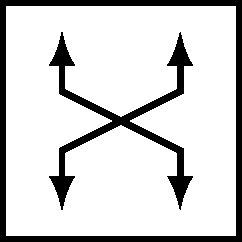
\includegraphics[width=0.9cm]{../common/fig-switch.pdf}
}
\providecommand{\router}{%
    
\includegraphics[width=0.9cm]{../common/fig-router.pdf}
}

\begin{frame}{bandwidth / throughput}
    \begin{itemize}
    \item bandwidth / data rate: maximum rate we can send per unit time
        \begin{itemize}
        \item most commonly measuring the speed of a link
        \end{itemize}
    \item 1 gigabit/second = transmit 1 bit / nanosecond
    \vspace{.5cm}
    \item throughput: acheived rate per unit time
        \begin{itemize}
        \item often lower than total bandwidth because of losses
        \item (we'll give several examples throughout the semester)
        \end{itemize}
    \end{itemize}
\end{frame}

\begin{frame}{latency (1)}
    \begin{itemize}
    \item latency: time for message: SOURCE $\rightarrow$ DEST
    \item example: \myemph<3>{1000} bit message from S to D:
    \end{itemize}
\begin{tikzpicture}
\tikzset{
    connect/.style={draw,very thick,Latex-Latex},
    computer/.style={inner sep=0mm,outer sep=0mm,execute at begin node={\computer}},
}
\node[computer,label={center:S}] (s) {};
\node[computer,label={center:D}] (d) at ([xshift=10cm]s.east) {};
\draw[connect] (s) -- (d) node[midway,above] {\myemph<2>{50 Mbit}, \myemph<3>{500 meters of copper}};
\end{tikzpicture}
\begin{itemize}
\item<2-> \myemph<2>{one} bit sent each \myemph<2>{1/50M second = 0.02 \mu s}
\item<2-> \myemph<3>{1000 bits take $0.02 \times 1000 = 20$ \mu s to sent}
    \begin{itemize}
    \item ``transmission delay''
    \end{itemize}
\item<3-> + $2.2$ microseconds for bit to go down cable ($2.3\times10^8$ m/s)
    \begin{itemize}
    \item ``propogation delay''
    \end{itemize}
\item<4-> total latency of about 22.2 \mu s
\end{itemize}
\end{frame}

\begin{frame}{latency (1, ex)}
\begin{tikzpicture}
\tikzset{
    connect/.style={draw,very thick,Latex-Latex},
    computer/.style={inner sep=0mm,outer sep=0mm,execute at begin node={\computer}},
    switch/.style={inner sep=0mm,outer sep=0mm,execute at begin node={\switch}},
}
\node[computer,label={center:S}] (s) {};
\node[computer,label={center:D}] (d) at ([xshift=10cm]s.east) {};
\draw[connect] (s) -- (d) node[midway,above] {\myemph{1 Gbit}, \myemph<3>{10 kilometers of fibre}};
\end{tikzpicture}
\begin{itemize}
\item exercise: latency for 20000 bit message from S to D
    \begin{itemize}
    \item assume speed of signal through fiber of $2.0\times10^8$ m/s
    \end{itemize}
\end{itemize}
\end{frame}

\begin{frame}{latency (2)}
    \begin{itemize}
    \item example: 1000 bit packet from S to D
    \item assume when message is received:
        \begin{itemize}
        \item 5 other 1000-bit packets in queue; no extra bits between packets
        \item no other switch processing time
        \end{itemize}
    \end{itemize}
\begin{tikzpicture}
\tikzset{
    connect/.style={draw,very thick,Latex-Latex},
    computer/.style={inner sep=0mm,outer sep=0mm,alt=<4>{label={[font=\small,label distance=0mm,text=red]south:`host'}},execute at begin node={\computer}},
    switch/.style={inner sep=0mm,outer sep=0mm,execute at begin node={\switch}},
}
\node[computer,label={center:S}] (s) {};
\node[switch] (m) at ([xshift=6.25cm]s.east) {};
\node[computer,label={center:D}] (d) at ([xshift=6.25cm]m.east) {};
\draw[connect] (s) -- (m) node[font=\small,midway,above] {50 Mbit, 500 meters of copper};
\draw[connect] (m) -- (d) node[font=\small,midway,above] {50 Mbit, 500 meters of copper};
\end{tikzpicture}
\begin{itemize}
\item latency from S to switch: 22.2 \mu s 
\item time waiting on switch: wait $20\times5=100$ \mu s for 5 other packets
    \begin{itemize}
    \item ``queueing delay''
    \end{itemize}
\item latency from switch to D: 22.2 \mu s 
\item total latency: $22.2 + 100 + 22.2 = 144.4$ microseconds
\end{itemize}
\end{frame}

\begin{frame}{round trip time}
    \begin{itemize}
    \item round-trip-time (RTT): time for message: SOURCE $\rightarrow$ DEST $\rightarrow$ SOURCE
    \end{itemize}
\end{frame}


\section{jitter}
\begin{frame}{jitter}
\begin{itemize}
\item variation in latency
    \begin{itemize}
    \item most commonly from changing queuing delays
    \end{itemize}
\end{itemize}
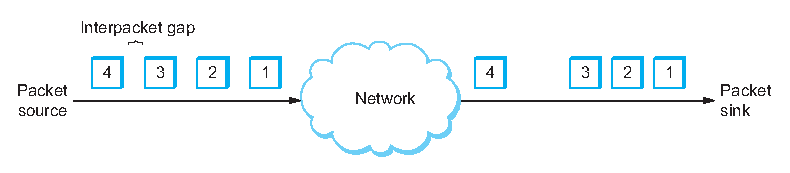
\includegraphics[width=0.9\textwidth]{../perf/SysApproach-1-Fig20}
\imagecredit{Figure 20 from Section 1.5 of \textit{Computer Networks: A Systems Approach} (6th ed) (Peterson and Davie)}
\end{frame}


\section{stop-and-wait performance}
\begin{frame}{stop-and-wait performance}
    \begin{itemize}
    \item stop-and-wait protocol
    \item assuming no packets lost/corrupted
    \vspace{.5cm}
    \item about \myemph{one packet per round-trip time}
    \end{itemize}
\end{frame}

\begin{frame}{example: local ethernet}
    \begin{itemize}
    \item my home wired network: 0.6 ms round trip time
    \item typical packet has about 1400 bytes = 11200 bits of data
    \item throughput with stop-and-wait: $11200 \text{b} / 0.6 \text{ms} \approx 19000 \text{b/ms} = 19\;000\;000 \text{b/s} = \myemph<2>{19 \text{Mbit/s}}$
    \vspace{.5cm}
    \item available bandwidth is about \myemph<2>{$1$ Gbit/s}
    \end{itemize}
\end{frame}


\section{sliding windows}

\subsection{sending two at a time}

\usetikzlibrary{arrows.meta,shapes.misc}
\begin{frame}{sending two at a time}
\begin{tikzpicture}
\tikzset{
    box/.style={thick},
    message/.style={draw,thick,-Latex},
    failure/.style={draw,ultra thick,red,cross out,minimum width=1cm,minimum height=1cm},
    every node/.style={inner sep=0.1mm},
}
\begin{scope}[xshift=1cm,x=0.9cm]
\draw[box] (0, 0) rectangle ++(2, -6) 
    node[midway,align=center] {machine\\A};
\draw[box] (13, 0) rectangle ++(2, -6) 
    node[midway,align=center] {machine\\B};
\draw[message] (2, -0.5) -- (13, -1.5) node[pos=0.25,above,sloped] {\myemph{0}: ``The ''};
\draw[message] (13, -1.75) -- (2, -2.75) node[pos=0.25,sloped,below] {got up to \myemph{0}};
\draw[message] (2, -1) -- (13, -2) node[pos=0.25, above, sloped] {\myemph{1}: ``meeting''};
\draw[message] (13, -2.25) -- (2, -3.25) node[pos=0.25, sloped,below] {got up to \myemph{1}};

% in response to got 0
\draw[message] (2, -3) -- (13, -4) node[pos=0.5, above, sloped] {\myemph{2}: `` is at ''};
\draw[message] (13, -4.25) -- (2, -5.25) node[pos=0.25, sloped,below] {got up to \myemph{2}};
% in response to got 1
\draw[message] (2, -3.5) -- (13, -4.5) node[pos=0.5, above, sloped] {\myemph{3}: ``12pm.''};
\draw[message] (13, -4.75) -- (2, -5.75) node[pos=0.25, sloped,below] {got up to \myemph{3}};
\end{scope}
\end{tikzpicture}
\begin{itemize}
\item key idea: always have two in flight
\item send next when previous ack'd
\end{itemize}
\end{frame}


\subsection{timeouts for EACH send}
\begin{frame}{timeouts per message} 
\begin{tikzpicture}
\tikzset{
    box/.style={thick},
    message/.style={draw,thick,-Latex},
    failure/.style={draw,ultra thick,red,cross out,minimum width=.5cm,minimum height=.5cm},
    every node/.style={inner sep=0.1mm},
}
\begin{scope}[xshift=1cm,x=0.9cm,y=0.7cm]
\draw[box] (0, 0) rectangle ++(2, -10) 
    node[midway,align=center] {machine\\A};
\draw[box] (13, 0) rectangle ++(2, -10) 
    node[midway,align=center] {machine\\B};
\draw[message] (2, -0.5) -- (13, -1.5) node[pos=0.25,above,sloped] {\myemph{0}: ``The ''};
\draw[message] (13, -1.75) -- (2, -2.75) node[pos=0.25,sloped,below] {ACK up to \myemph{0}};
\draw[message] (2, -1) -- (9, -1.75) node[pos=0.25, above, sloped] {\myemph{1}: ``meeting''}
    node[failure] {};
%\draw[message] (13, -2.25) -- (2, -3.25) node[pos=0.25, sloped,below] {got \myemph{1}};

% in response to got 0
\draw[message] (2, -3) -- (13, -4) node[pos=0.5, above, sloped] {\myemph{2}: `` is at ''};
%\draw[message] (13, -4.25) -- (2, -5.25) node[pos=0.25, sloped,below,alt=<2>{draw=red,ultra thick}] {ACK up to \myemph{0}};
\draw[message,opacity=0.25] (13, -4.25) -- (2, -5.25) node[pos=0.25, sloped,below] {ACK up to \myemph{0}};

\draw[ultra thick,red,decorate,decoration={brace}] (2.1, -1) -- (2.1, -6) node[pos=0.4,right=0.5cm] {\bfseries timeout for 1};
\draw[message] (2, -6) -- (13, -7) node[pos=0.5, above, sloped] {\myemph{1}: ``meeting''};
\draw[message] (13, -7.25) -- (2, -8.25) node[pos=0.25, sloped,below] {ACK \myemph{1}};
\draw[message] (2, -8.5) -- (13, -9.5) node[pos=0.5, above, sloped] {\myemph{3}: `` 12pm ''};

\draw[ultra thick,red,decorate,decoration={brace}] (2.4, -3) -- (2.4, -7.5) node[pos=0.5,right=0.5cm] {\bfseries timeout for 2};
\draw[message] (2, -7.5) -- (13, -8.5) node[pos=0.5, above, sloped] {\myemph{2}: `` is at ''};
\end{scope}
\end{tikzpicture}
\end{frame}


\subsection{more than two at a time}
\begin{frame}{sending three at a time}
\begin{tikzpicture}
\tikzset{
    box/.style={thick},
    message/.style={draw,thick,-Latex},
    failure/.style={draw,ultra thick,red,cross out,minimum width=1cm,minimum height=1cm},
    every node/.style={inner sep=0.1mm},
}
\begin{scope}[xshift=1cm,x=0.9cm]
\draw[box] (0, 0) rectangle ++(2, -6) 
    node[midway,align=center] {machine\\A};
\draw[box] (13, 0) rectangle ++(2, -6) 
    node[midway,align=center] {machine\\B};
\draw[message] (2, -0.5) -- (13, -1.5) node[pos=0.25,above,sloped] {\myemph{0}: ``The ''};
\draw[message] (13, -1.75) -- (2, -2.75) node[pos=0.25,sloped,below] {got up to \myemph{0}};
\draw[message] (2, -1) -- (13, -2) node[pos=0.25, above, sloped] {\myemph{1}: ``meeting''};
\draw[message] (13, -2.25) -- (2, -3.25) node[pos=0.25, sloped,below] {got up to \myemph{1}};
\draw[message] (2, -2) -- (13, -3) node[pos=0.5, above, sloped] {\myemph{2}: `` is at ''};
\draw[message] (13, -3.25) -- (2, -4.25) node[pos=0.25, sloped,below] {got up to \myemph{2}};
% in response to got 0
\draw[message] (2, -3) -- (13, -4.5) node[pos=0.5, above, sloped] {\myemph{3}: ``12pm.''};
\draw[message] (13, -4.75) -- (2, -5.75) node[pos=0.25, sloped,below] {got up to \myemph{3}};
% in response to got 1 
\draw[message] (2, -3.5) -- (13, -4.5) node[pos=0.5, above, sloped] {\myemph{4}: ``Please ''};
\draw[message] (13, -4.75) -- (2, -5.75) node[pos=0.25, sloped,below] {got up to \myemph{4}};
\draw[message] (2, -4) -- (13, -5) node[pos=0.5, above, sloped] {\myemph{5}: ``be ''};
\draw[message] (13, -5.25) -- (2, -6.25) node[pos=0.25, sloped,below] {got up to \myemph{5}};
\draw[message] (2, -4.5) -- (13, -5.5) node[pos=0.5, above, sloped] {\myemph{6}: ``prompt ''};
\draw[message] (13, -5.75) -- (2, -6.75) node[pos=0.25, sloped,below] {got up to \myemph{6}};
\draw[message] (2, -7) -- (13, -5.5) node[pos=0.5, above, sloped] {\myemph{7}: \ldots};
\end{scope}
\end{tikzpicture}
\begin{itemize}
\item choose ``window size'' to have in flight
\item send when previous acknowledged
\end{itemize}
\end{frame}


\subsection{lost ACKs}
\begin{frame}{lost ACKs?}
\begin{tikzpicture}
\tikzset{
    box/.style={thick},
    message/.style={draw,thick,-Latex},
    failure/.style={draw,ultra thick,red,cross out,minimum width=1cm,minimum height=1cm},
    every node/.style={inner sep=0.1mm},
}
\begin{scope}[xshift=1cm,x=0.9cm]
\draw[box] (0, 0) rectangle ++(2, -6) 
    node[midway,align=center] {machine\\A};
\draw[box] (13, 0) rectangle ++(2, -6) 
    node[midway,align=center] {machine\\B};
\draw[message] (2, -0.5) -- (13, -1.5) node[pos=0.25,above,sloped] {\myemph{0}: ``The ''};
\draw[message] (13, -1.75) -- (2, -2.75) node[pos=0.25,sloped,below] {ACK up to \myemph{0}};
\draw[message] (2, -1) -- (13, -2) node[pos=0.25, above, sloped] {\myemph{1}: ``meeting''};
\draw[message] (13, -2.25) -- (5, -3) node[pos=0.25, sloped,below] {ACK up to \myemph{1}} node[failure] {};
\draw[message] (2, -1.5) -- (13, -2.5) node[pos=0.25, above, sloped] {\myemph{2}: `` is at ''};
\draw[message] (13, -2.75) -- (2, -3.75) node[pos=0.25, sloped,below] {ACK up to \myemph{2}};
\draw[message] (2, -3) -- (13, -4) node[pos=0.5, above, sloped] {\myemph{3}: ``12pm.''};
\draw[message] (13, -4.25) -- (2, -5.25) node[pos=0.25, sloped,below] {ACK up to \myemph{3}};
\draw[message] (2, -4) -- (13, -5) node[pos=0.5, above, sloped] {\myemph{4}: ``Please ''};
\draw[message] (13, -5.25) -- (2, -6) node[pos=0.25, sloped,below] {ACK up to \myemph{4}};
\draw[message] (2, -4.5) -- (13, -5.5) node[pos=0.5, above, sloped] {\myemph{5}: ``be ''};
\draw[message] (13, -5.75) -- (2, -6.5) node[pos=0.25, sloped,below] {ACK up to \myemph{5}};
%\draw[message] (2, -4.5) -- (13, -5.5) node[pos=0.5, above, sloped] {\myemph{6}: ``prompt ''};
%\draw[message] (13, -5.75) -- (2, -6.75) node[pos=0.25, sloped,below] {ACK up to \myemph{6}};
%\draw[message] (2, -7) -- (13, -5.5) node[pos=0.5, above, sloped] {\myemph{7}: \ldots};
\end{scope}
\end{tikzpicture}
\end{frame}


\subsection{duplicate ACKs happen}
    % FIXME: this would make more sense with more than two things
\usetikzlibrary{decorations.pathreplacing}
\begin{frame}<1-2>[label=twoAndTimeouts]{missing messages?}
\begin{tikzpicture}
\tikzset{
    box/.style={thick},
    message/.style={draw,thick,-Latex},
    failure/.style={draw,ultra thick,red,cross out,minimum width=.5cm,minimum height=.5cm},
    every node/.style={inner sep=0.1mm},
}
\begin{scope}[xshift=1cm,x=0.9cm]
\draw[box] (0, 0) rectangle ++(2, -4) 
    node[midway,align=center] {machine\\A};
\draw[box] (13, 0) rectangle ++(2, -4) 
    node[midway,align=center] {machine\\B};
\draw[message] (2, -0.5) -- (13, -1.5) node[pos=0.25,above,sloped] {\myemph{0}: ``The ''};
\draw[message] (13, -1.75) -- (2, -2.75) node[pos=0.25,sloped,below] {got up to \myemph{0}};
\draw[message] (2, -1) -- (9, -1.7) node[pos=0.25, above, sloped] {\myemph{1}: ``meeting''}
    node[failure] {};
%\draw[message] (13, -2.25) -- (2, -3.25) node[pos=0.25, sloped,below] {got \myemph{1}};

% in response to got 0
\draw[message,draw=red,ultra thick] (2, -3) -- (13, -4) node[pos=0.5, above, sloped] {\myemph{2}: `` is at ''};
%\draw[message] (13, -4.25) -- (2, -5.25) node[pos=0.25, sloped,below,alt=<2>{draw=red,ultra thick}] {got up to \myemph{0}};
%\draw[message] (2, -3.5) -- (13, -4.5) node[pos=0.5, above, sloped] {\myemph{3}: ``12pm.''};
%\draw[message] (13, -4.75) -- (2, -5.75) node[pos=0.25, sloped,below] {got \myemph{3}};
\end{scope}
\end{tikzpicture}
\begin{itemize}
\item question: what should receiver do with sequence number 2?
\item<2-> \myemph<2>{one idea: ignore it?}
\item<3-> \myemph<3>{better idea: send something back to sender}
\end{itemize}
\end{frame}

\begin{frame}<0>{not great: ignore it (1)} 
\begin{tikzpicture}
\tikzset{
    box/.style={thick},
    message/.style={draw,thick,-Latex},
    failure/.style={draw,ultra thick,red,cross out,minimum width=.5cm,minimum height=.5cm},
    every node/.style={inner sep=0.1mm},
}
\begin{scope}[xshift=1cm,x=0.9cm,y=0.7cm]
\draw[box] (0, 0) rectangle ++(2, -10) 
    node[midway,align=center] {machine\\A};
\draw[box] (13, 0) rectangle ++(2, -10) 
    node[midway,align=center] {machine\\B};
\draw[message] (2, -0.5) -- (13, -1.5) node[pos=0.25,above,sloped] {\myemph{0}: ``The ''};
\draw[message] (13, -1.75) -- (2, -2.75) node[pos=0.25,sloped,below] {got up to \myemph{0}};
\draw[message] (2, -1) -- (9, -1.75) node[pos=0.25, above, sloped] {\myemph{1}: ``meeting''}
    node[failure] {};
%\draw[message] (13, -2.25) -- (2, -3.25) node[pos=0.25, sloped,below] {got \myemph{1}};

% in response to got 0
\draw[message] (2, -3) -- (13, -4) node[pos=0.5, above, sloped] {\myemph{2}: `` is at ''};
%\draw[message] (13, -4.25) -- (2, -5.25) node[pos=0.25, sloped,below,alt=<2>{draw=red,ultra thick}] {got up to \myemph{0}};
\draw[ultra thick,red,decorate,decoration={brace}] (2.1, -1) -- (2.1, -6) node[pos=0.4,right=0.5cm] {\bfseries timeout for 1};
\draw[message] (2, -6) -- (13, -7) node[pos=0.5, above, sloped] {\myemph{1}: ``meeting''};
\draw[message] (13, -7.25) -- (2, -8.25) node[pos=0.25, sloped,below] {got \myemph{1}};
\draw[message] (2, -8.5) -- (13, -9.5) node[pos=0.5, above, sloped] {\myemph{3}: `` 12pm ''};

\draw[ultra thick,red,decorate,decoration={brace}] (2.4, -3) -- (2.4, -7.5) node[pos=0.5,right=0.5cm] {\bfseries timeout for 2};
\draw[message] (2, -7.5) -- (13, -8.5) node[pos=0.5, above, sloped] {\myemph{2}: `` is at ''};
\end{scope}
\end{tikzpicture}
\end{frame}

\begin{frame}<0>{not great: only ACK if next (2)}
    \begin{itemize}
    \item \textit{works} because we still have timeouts
    \vspace{.5cm}
    \item but we'd like to give more feedback to receiver
    \end{itemize}
\end{frame}

\againframe<3>{twoAndTimeouts}

\begin{frame}{better idea: always ACK}
\begin{tikzpicture}
\tikzset{
    box/.style={thick},
    message/.style={draw,thick,-Latex},
    failure/.style={draw,ultra thick,red,cross out,minimum width=1cm,minimum height=1cm},
    every node/.style={inner sep=0.1mm},
}
\begin{scope}[xshift=1cm,x=0.9cm]
\draw[box] (0, 0) rectangle ++(2, -5.5) 
    node[midway,align=center] {machine\\A};
\draw[box] (13, 0) rectangle ++(2, -5.5) 
    node[midway,align=center] {machine\\B};
\draw[message] (2, -0.5) -- (13, -1.5) node[pos=0.25,above,sloped] {\myemph{0}: ``The ''};
\draw[message] (13, -1.75) -- (2, -2.75) node[pos=0.25,sloped,below] {got up to \myemph{0}};
\draw[message] (2, -1) -- (9, -1.7) node[pos=0.25, above, sloped] {\myemph{1}: ``meeting''}
    node[failure] {};
%\draw[message] (13, -2.25) -- (2, -3.25) node[pos=0.25, sloped,below] {got \myemph{1}};

% in response to got 0
\draw[message] (2, -3) -- (13, -4) node[pos=0.5, above, sloped] {\myemph{2}: `` is at ''};
\draw[message] (13, -4.25) -- (2, -5.25) node[pos=0.25, sloped,below,alt=<2>{draw=red,ultra thick}] {got up to \myemph{0}};
%\draw[message] (2, -3.5) -- (13, -4.5) node[pos=0.5, above, sloped] {\myemph{3}: ``12pm.''};
%\draw[message] (13, -4.75) -- (2, -5.75) node[pos=0.25, sloped,below] {got \myemph{3}};
\end{scope}
\end{tikzpicture}
\begin{itemize}
\item<2-> only ACK $x$ if \myemph{everything up to and including $x$} received
\item<2-> intuition: ACK tells sender \myemph{where to start sending more}
\end{itemize}
\end{frame}


\subsection{duplicate ACK optimization}
\begin{frame}{fast retransmit}
    \begin{itemize}
    \item if large window + data packet 2 is lost, then sender will see
    \item ACK 0, \myemph{ACK 1, ACK 1, ACK 1, ACK 1, ACK 1}
    \item duplicate ACKs indicate missing packet 2
    \item \myemph{shouldn't wait for timeout}
    \vspace{.5cm}
    \item<2-> $\rightarrow$ TCP heuristic: retransmit immediately after $\sim$3 duplicate ACKs
        \begin{itemize}
        \item not 1 duplicate ACK to tolerate some reordering
        \item also some other details (we'll talk later)
        \end{itemize}
    \end{itemize}
\end{frame}



\subsection{optimization: selective ACKs}
\begin{frame}{multiple missing}
\begin{tikzpicture}
\tikzset{
    box/.style={thick},
    message/.style={draw,thick,-Latex},
    failure/.style={draw,ultra thick,red,cross out,minimum width=1cm,minimum height=1cm},
    every node/.style={inner sep=0.1mm},
}
\begin{scope}[xshift=1cm,x=0.9cm]
\draw[box] (0, 0) rectangle ++(2, -5.5) 
    node[midway,align=center] {machine\\A};
\draw[box] (13, 0) rectangle ++(2, -5.5) 
    node[midway,align=center] {machine\\B};
\draw[message] (2, -0.5) -- (13, -1.5) node[pos=0.25,above,sloped] {\myemph{0}: ``The ''};
\draw[message] (13, -1.75) -- (2, -2.75) node[pos=0.25,sloped,below] {got up to \myemph{0}};
\draw[message] (2, -1) -- (9, -1.7) node[pos=0.25, above, sloped] {\myemph{1}: ``meeting''}
    node[failure] {};
\draw[message] (2, -1.5) -- (13, -2) node[pos=0.5, above, sloped] {\myemph{2}: ``is''};
\draw[message] (2, -2) -- (13, -3) node[pos=0.5, above, sloped] {\myemph{3}: ``at''}
    node[failure] {};
\draw[message] (2, -3) -- (13, -4) node[pos=0.5, above, sloped] {\myemph{4}: ``12pm''};

\draw[message] (13, -2.25) -- (2, -3.25) node[pos=0.25, sloped,below,alt=<2>{draw=red,ultra thick}] {got up to \myemph{0}};
\draw[message] (13, -3.25) -- (2, -4.25) node[pos=0.25, sloped,below,alt=<2>{draw=red,ultra thick}] {got up to \myemph{0}};
\end{scope}
\end{tikzpicture}
\begin{itemize}
\item duplicate ACK heuristic will quickly resend 1, but not 3
\item would like to supply better information
\end{itemize}
\end{frame}

\begin{frame}{selective acknowledgments}
\begin{tikzpicture}
\tikzset{
    box/.style={thick},
    message/.style={draw,thick,-Latex},
    failure/.style={draw,ultra thick,red,cross out,minimum width=1cm,minimum height=1cm},
    every node/.style={inner sep=0.1mm},
}
\begin{scope}[xshift=1cm,x=0.9cm]
\draw[box] (0, 0) rectangle ++(2, -5.5) 
    node[midway,align=center] {machine\\A};
\draw[box] (13, 0) rectangle ++(2, -5.5) 
    node[midway,align=center] {machine\\B};
\draw[message] (2, -0.5) -- (13, -1.5) node[pos=0.25,above,sloped] {\myemph{0}: ``The ''};
\draw[message] (13, -1.75) -- (2, -2.75) node[pos=0.25,sloped,below] {got up to \myemph{0}};
\draw[message] (2, -1) -- (9, -1.7) node[pos=0.25, above, sloped] {\myemph{1}: ``meeting''}
    node[failure] {};
\draw[message] (2, -1.5) -- (13, -2) node[pos=0.5, above, sloped] {\myemph{2}: ``is''};
\draw[message] (2, -2) -- (13, -3) node[pos=0.5, above, sloped] {\myemph{3}: ``at''}
    node[failure] {};
\draw[message] (2, -3) -- (13, -4) node[pos=0.5, above, sloped] {\myemph{4}: ``12pm''};

\draw[message] (13, -2.25) -- (2, -3.25) node[pos=0.25, sloped,below,alt=<2>{draw=red,ultra thick}] {got up to \myemph{0} plus 2};
\draw[message] (13, -3.25) -- (2, -4.25) node[pos=0.25, sloped,below,alt=<2>{draw=red,ultra thick}] {got up to \myemph{0} plus 2 and 4};
\end{scope}
\end{tikzpicture}
\end{frame}

\begin{frame}{selective acknowledgments in TCP}
    \begin{itemize}
    \item optional feature (``extension'') described in RFC 2018
    \item send list of ranges received
    \item typically room for 3 ranges
    \item if more than 3 ranges to report, then:
        \begin{itemize}
        \item include range with most recently received frame
        \item include other ranges until sent three times
        \end{itemize}
    \end{itemize}
\end{frame}


\subsection{window tracking -- sender}
% FIXME: diagram of receiver, sender window
    % actions for each case
\usetikzlibrary{arrows.meta,decorations.pathreplacing,matrix,patterns}
\begin{frame}{sender window tracking}
\begin{tikzpicture}
\tikzset{
    seqlist/.style={tight matrix,nodes={text width=1cm,minimum height=1cm},column sep=.8mm},
    dots/.style={draw=none,execute at begin node=\ldots,anchor=center,font=\huge,text width=1cm,align=center},
    region mark/.style={very thick,decorate,decoration={brace,mirror}},
    region mark label/.style={midway,below,align=center},
    verified/.style={alt=<2->{pattern color=black!30,pattern=checkerboard}},
    in flight/.style={alt=<3->{fill=yellow}},
    unsent/.style={alt=<4->{pattern=crosshatch dots,pattern color=violet!70}}
}
\matrix[seqlist] (swindow) {
    |[dots,alias=swindow-start]| ~ \& |[alias=after-swindow-start,verified]| ~ \& |[verified]|  ~\&
   |[verified]| ~ \& |[alias=LFA,verified]| ~ \&
    |[in flight,alias=after LFA]| ~ \& |[in flight]| ~ \& |[in flight]| ~ \& |[in flight,alias=LFS]| ~ \& 
    |[alias=after LFS,unsent]| ~ \& |[unsent,alias=before-swindow-end]| ~ \& |[alias=swindow-end,dots]| \\
};
\matrix[anchor=north west,seqlist,label={east:= frame of data with sequeunce number $X$}] (key) at ([yshift=2.5cm]swindow.north west) { ~ \\};
    \node[font=\small,anchor=south west,inner sep=0.1mm] at (key-1-1.north west) {$X$};
\foreach \x in {2,...,11} {
    \pgfmathtruncatemacro\xplus{\x + 10}
    \node[font=\small,anchor=south west,inner sep=0.1mm] at (swindow-1-\x.north west) {\xplus};
}
\draw[thick,Latex-] (LFA.north) -- ++(0,.5) node[above,align=center] {(LAR)\\last ACK recv'd};
\draw[thick,Latex-] (LFS.north) -- ++(0,.5) node[above,align=center] {(LFS)\\last frame sent};
\begin{visibleenv}<2->
    \draw[region mark] ([yshift=-.1cm]swindow-start.south west) -- ([yshift=-.1cm]LFA.south east)
        node[region mark label] {verified received \\ can discard};
\end{visibleenv}
\begin{visibleenv}<3->
    \draw[region mark] ([yshift=-.1cm]after LFA.south west) -- ([yshift=-.1cm]LFS.south east)
        node[region mark label] (in flight label) {might need to resend \\ potentially ``in flight''};
    \begin{visibleenv}<5->
    \draw[thick,Latex-] (in flight label.south) -- ++(0,-.5) node[below,align=center] {
            at most the \\
            Send Window Size \\
            (SWS)
        };
    \end{visibleenv}
\end{visibleenv}
\begin{visibleenv}<4->
    \draw[region mark] ([yshift=-.1cm]after LFS.south west) -- ([yshift=-.1cm]swindow-end.south east)
        node[region mark label] {yet to be sent};
\end{visibleenv}
\end{tikzpicture}
\end{frame}

\begin{frame}{exercise 1: out-of-bounds ACK}
\begin{tabular}{l|l}
last ACK recv'd (LAR) & 10 \\
last frame sent (LFS) & 15 \\
send window size (SWS) & 5 \\
\end{tabular}
\begin{itemize}
\item what probably happened if we receive an ACK for\ldots
    \begin{itemize}
    \item 9? 10? 13? 16?
    \end{itemize}
\end{itemize}
\begin{tabular}{l}
A. only possible if network reorders frames \\
B. only possible from undetected frame corruption \\
C. lost ACK for frame $\le$ 10\\
D. lost ACK for frame $>$ 10\\
E. lost frame 11 \\
F. resent frame from timeout \\
\end{tabular}
\end{frame}

\begin{frame}{exercise 2: sender logic}
\begin{tabular}{l|l}
last ACK recv'd (LAR) & 10 \\
last frame sent (LFS) & 15 \\
send window size (SWS) & 5 \\
\end{tabular}
\begin{itemize}
\item In this case, there's a timeout that will
trigger frame 13 to be resent. If still active,
this timeout should be cancelled upon \ldots
\end{itemize}
\begin{tabular}{ll}
A. receiving ACK 12 & B. receiving ACK 13 \\
C. receiving ACK 14 & D. sending frame 16 \\
\end{tabular}
\end{frame}

\begin{frame}{exercise 3a: new data}
\begin{tabular}{l|l}
last ACK recv'd (LAR) & 4 \\
last frame sent (LFS) & 6 \\
send window size (SWS) & 5 \\
\end{tabular}
\begin{itemize}
\item if we compute a new frame of data with sequence number 7 to eventually
send, we should
\end{itemize}
\begin{tabular}{l}
A. send it now, advancing LFS \\
B. wait until we get an ACK for 5 or 6 to send it \\
C. wait until we get an ACK for 6 to send it \\
D. wait until the frame with sequence number 6 is resent to send it
D. something else \\
\end{tabular}
\end{frame}

\begin{frame}{exercise 3b: new data}
\begin{tabular}{l|l}
last ACK recv'd (LAR) & 4 \\
last frame sent (LFS) & 8 \\
send window size (SWS) & 4 \\
\end{tabular}
\begin{itemize}
\item if we compute a new frame of data with sequence number 9 to eventually
send, we should
\end{itemize}
\begin{tabular}{l}
A. send it now, advancing LFS \\
B. wait until we get an ACK for 5 or 6 to send it \\
C. wait until we get an ACK for 6 to send it \\
D. decline to accept the data because we will never be able to send it \\
E. something else \\
\end{tabular}
\end{frame}

\begin{frame}{sender logic summarized}
\begin{itemize}
\item track variables:
    \begin{itemize}
    \item LFS (last frame sent)
    \item LAS (last ACK recv'd)
    \item SWS (send window size)
    \end{itemize}
\item when receiving ACK $LAR < X \le LFS$:
    \begin{itemize}
    \item LAR $\leftarrow$ $X$
    \item clear any timers to resend frames $\le X$
    \end{itemize}
\item whenever SWS [send window size] > LFS - LAR \textit{and} \\
    data for frame LFS + 1 is available:
    \begin{itemize}
    \item send frame LFS + 1
    \item set timer to resend frame LFS + 1
    \item LFS $\leftarrow$ LFS + 1
    \end{itemize}
\end{itemize}
\end{frame}


\subsection{window tracking -- receiver}
\usetikzlibrary{arrows.meta,decorations.pathreplacing,matrix,patterns}
\begin{frame}{receiver window tracking}
\begin{tikzpicture}
\tikzset{
    seqlist/.style={tight matrix,nodes={text width=1cm,minimum height=1cm},column sep=.9mm},
    dots/.style={draw=none,execute at begin node=\ldots,anchor=center,font=\huge,text width=1cm,align=center},
    region mark/.style={very thick,decorate,decoration={brace,amplitude=1mm,mirror}},
    region mark label/.style={midway,below,align=center},
    verified/.style={alt=<2->{pattern color=black!30,pattern=checkerboard}},
    missing/.style={alt=<3->{pattern color=yellow,pattern=north west lines}},
    in flight/.style={alt=<3->{fill=yellow}},
    unsent/.style={alt=<4->{pattern=crosshatch dots,pattern color=violet!70}}
}
\matrix[seqlist] (swindow) {
    |[dots,alias=swindow-start]| ~ \& |[alias=after-swindow-start,verified]| ~ \& |[verified]|  ~\&
   |[verified]| ~ \& |[alias=LFR,verified]| ~ \&
    |[missing,alias=after LFR]| ~ \& |[in flight,alias=after after LFR]| ~ \&
    |[in flight]| ~ \& |[in flight,alias=LAF]| ~ \& 
    |[alias=after LAF,unsent]| ~ \& |[unsent,alias=before-swindow-end]| ~ \& |[alias=swindow-end,dots]| \\
};
\matrix[anchor=north west,seqlist,label={east:= frame of data with sequeunce number $X$}] (key) at ([yshift=2.5cm]swindow.north west) { ~ \\};
    \node[font=\small,anchor=south west,inner sep=0.1mm] at (key-1-1.north west) {$X$};
\foreach \x in {2,...,11} {
    \pgfmathtruncatemacro\xplus{\x + 10}
    \node[font=\small,anchor=south west,inner sep=0.1mm] at (swindow-1-\x.north west) {\xplus};
}
\draw[thick,Latex-] (LFR.north) -- ++(0,.5) node[above,align=center] {(LFR)\\last frame recv'd*};
\draw[thick,Latex-] (LAF.north) -- ++(0,.5) node[above,align=center] {(LAF)\\last accepted frame};
\begin{visibleenv}<2->
    \draw[region mark] ([yshift=-.1cm]swindow-start.south west) -- ([yshift=-.1cm]LFR.south east)
        node[region mark label] {already received};
\end{visibleenv}
\begin{visibleenv}<3->
    \draw[thick,Latex-] (after LFR.south) -- ++(0,-.3) node[below,align=center] { not\\recv'd };
    \draw[region mark] ([yshift=-.1cm]after after LFR.south west) -- ([yshift=-.1cm]LAF.south east)
        node[region mark label,below=1mm] (label) {accepted \\ possibly recv'd};
\end{visibleenv}
\begin{visibleenv}<4->
    \draw[region mark] ([yshift=-1.6cm]after LFR.south west) -- ([yshift=-1.6cm]LAF.south east)
        node[region mark label] (in flight label) {
            at most the \\
            Receive Window Size \\
            (RWS)
        };
\end{visibleenv}
\begin{visibleenv}<5->
    \draw[region mark] ([yshift=-.1cm]after LAF.south west) -- ([yshift=-.1cm]swindow-end.south east)
        node[region mark label] {will discard \\ too far ahead};
\end{visibleenv}
\end{tikzpicture}
\end{frame}

\begin{frame}{receiver logic summarized}
\begin{itemize}
\item track variables:
    \begin{itemize}
    \item LFR (last frame recv'd) --- excludes frames after a missing frame
    \item LAF (last accepted frame)
    \item RWS (receive window size)
    \end{itemize}
\item when receiving frame $LFR < X \le LAF$:
\item LFR $\leftarrow$ (first missing frame after LFR) - 1
    \begin{itemize}
    \item only advances if X $=$ LFR
    \item could advance by more than one if frames previously out of order
    \end{itemize}
\item LAS $\leftarrow$ LFR + RWS
    \begin{itemize}
    \item only advances if X $=$ LFR
    \end{itemize}
\end{itemize}
\end{frame}


\subsection{choosing a window size}
    % FIXME: graph of empirical performance

\usetikzlibrary{arrows.meta,calc}

\begin{frame}{simple network model}
\begin{tikzpicture}
\draw[ultra thick,arrows={-Latex}] (0, 0) node[left] {sender} -- (1, 0);
\draw[thick] (1, -.5) rectangle (3, .5);
\foreach \x in {2,2.2,2.4,2.6,2.8} {
    \draw (\x, -.5) -- (\x, .5);
}
\node[anchor=south,align=center] at (2, .5) {
    loss when full
};
\node[anchor=north,align=center] at (2, -.5) (queue label) {
    queue
};
\node[anchor=north,font=\small] at ([yshift=.2cm]queue label.south) {
    capacity 20
};
\draw[ultra thick,arrows={-Latex}] (3, 0) -- (10, 0) node[right]{receiver}
    node[midway,fill=white,draw=black,very thick,align=left] {
        10 data frames/time unit \\
        1 time unit delay
    };
\begin{scope}[shift={(10, -3)},x=-1cm]
    \draw[ultra thick,arrows={-Latex}] (0, 0) node[right] {receiver} -- (1, 0);
    \draw[thick] (1, -.5) rectangle (3, .5);
    \foreach \x in {2,2.2,2.4,2.6,2.8} {
        \draw (\x, -.5) -- (\x, .5);
    }
    \node[anchor=south,align=center] at (2, .5) {
        loss when full
    };
    \node[anchor=north,align=center] at (2, -.5) (queue label) {
        queue
    };
    \node[anchor=north,font=\small] at ([yshift=.2cm]queue label.south) {
        capacity 20
    };
    \draw[ultra thick,arrows={-Latex}] (3, 0) -- (10, 0) node[left]{sender}
        node[midway,fill=white,draw=black,very thick,align=left] {
            100 ACK frames/time unit \\
            1 time unit delay
        };
\end{scope}
\end{tikzpicture}
\begin{itemize}
\item simulator from upcoming assignment
    \begin{itemize}
    \item command line \texttt{--delay 1 --bandwidth-forward 10 --bandwidth-backward 100 --buffer 30}
    \end{itemize}
\end{itemize}
\end{frame}

\begin{frame}{exercise: forward latency}
\begin{tikzpicture}
\draw[ultra thick,arrows={-Latex}] (0, 0) node[left] {sender} -- (1, 0);
\draw[thick] (1, -.5) rectangle (3, .5);
\foreach \x in {2,2.2,2.4,2.6,2.8} {
    \draw (\x, -.5) -- (\x, .5);
}
\node[anchor=south,align=center] at (2, .5) {
    loss when full
};
\node[anchor=north,align=center] at (2, -.5) (queue label) {
    queue
};
\node[anchor=north,font=\small] at (queue label.south) {
    capacity 10
};
\draw[ultra thick,arrows={-Latex}] (3, 0) -- (10, 0) node[right]{receiver}
    node[midway,fill=white,draw=black,very thick,align=left] {
        10 frames/time unit \\
        1 time unit delay \\
        \small (from transmit start)
    };
\end{tikzpicture}
\begin{itemize}
\item minimum latency = 1 time unit
\item exercise: maximum latency?
\end{itemize}
\begin{tabular}{lll}
A. 1 time unit & B. 1.1 time unit & C. 1.2 time unit \\
C. 1.4 time unit & D. 1.9 time unit & E. 2.0 time unit \\
F. 2.1 time unit & G. something else \\
\end{tabular}
\end{frame}

\usetikzlibrary{arrows.meta,calc}

\begin{frame}[fragile,label=throughAndWindow]{throughput and window size}
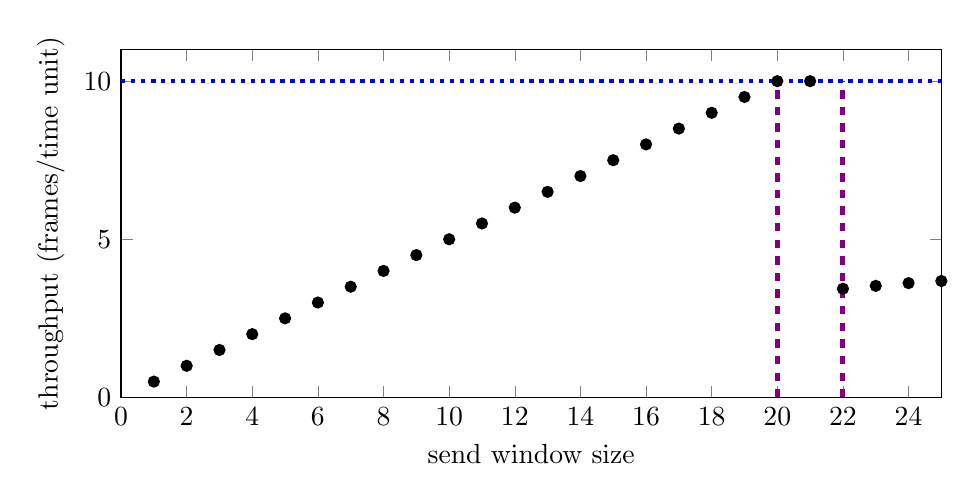
\begin{tikzpicture}
\begin{axis}[width=12cm,height=6cm,
    xlabel=send window size,
    ylabel=throughput (frames/time unit),
    xmin=0,xmax=25,ymin=0]
\addplot[only marks] coordinates {
(1, 0.5000025000125)
(2, 1.0000090000810007)
(3, 1.4999925000374998)
(4, 2.0000280003920055)
(5, 2.500037500562508)
(6, 3.000003000003)
(7, 3.5000035000035)
(8, 4.000048000576006)
(9, 4.499842505512307)
(10, 5.000025000125)
(11, 5.499975250111374)
(12, 5.99977200866367)
(13, 6.499710762871052)
(14, 6.999811005102861)
(15, 7.4996812635462975)
(16, 7.999680012799485)
(17, 8.499426288725509)
(18, 8.999361045365776)
(19, 9.499202067026369)
(20, 9.999100080971061)
(21, 9.999100080973866)
(22, 3.435635094325549)
(23, 3.5274986154570636)
(24, 3.613708966335035)
(25, 3.6808686850100703)
(26, 3.753260645186032)
(27, 3.8487443471573166)
(28, 3.925956461143474)
};
\addplot[blue,dotted,ultra thick,domain=0:25] {10};
    \draw[violet,dashed,ultra thick] (axis cs:20,0) -- (axis cs:20, 10)
     coordinate (empty queue mark);
    \draw[violet,dashed,ultra thick] (axis cs:21.99,0) -- (axis cs:21.99, 10)
     coordinate (full queue mark);
\end{axis}
\end{tikzpicture}
\end{frame}

\usetikzlibrary{arrows.meta,calc}

\begin{frame}{simple network model}
\begin{tikzpicture}
\draw[ultra thick,arrows={-Latex}] (0, 0) node[left] {sender} -- (1, 0);
\draw[thick] (1, -.5) rectangle (3, .5);
\foreach \x in {2,2.2,2.4,2.6,2.8} {
    \draw (\x, -.5) -- (\x, .5);
}
\node[anchor=south,align=center] at (2, .5) {
    loss when full
};
\node[anchor=north,align=center] at (2, -.5) (queue label) {
    queue
};
\node[anchor=north,font=\small] at ([yshift=.2cm]queue label.south) {
    capacity 20
};
\draw[ultra thick,arrows={-Latex}] (3, 0) -- (10, 0) node[right]{receiver}
    node[midway,fill=white,draw=black,very thick,align=left] {
        10 data frames/time unit \\
        1 time unit delay
    };
\begin{scope}[shift={(10, -3)},x=-1cm]
    \draw[ultra thick,arrows={-Latex}] (0, 0) node[right] {receiver} -- (1, 0);
    \draw[thick] (1, -.5) rectangle (3, .5);
    \foreach \x in {2,2.2,2.4,2.6,2.8} {
        \draw (\x, -.5) -- (\x, .5);
    }
    \node[anchor=south,align=center] at (2, .5) {
        loss when full
    };
    \node[anchor=north,align=center] at (2, -.5) (queue label) {
        queue
    };
    \node[anchor=north,font=\small] at ([yshift=.2cm]queue label.south) {
        capacity 20
    };
    \draw[ultra thick,arrows={-Latex}] (3, 0) -- (10, 0) node[left]{sender}
        node[midway,fill=white,draw=black,very thick,align=left] {
            100 ACK frames/time unit \\
            1 time unit delay
        };
\end{scope}
\end{tikzpicture}
\begin{itemize}
\item simulator from upcoming assignment
    \begin{itemize}
    \item command line \texttt{--delay 1 --bandwidth-forward 10 --bandwidth-backward 100 --buffer 30}
    \end{itemize}
\end{itemize}
\end{frame}

\begin{frame}{exercise: forward latency}
\begin{tikzpicture}
\draw[ultra thick,arrows={-Latex}] (0, 0) node[left] {sender} -- (1, 0);
\draw[thick] (1, -.5) rectangle (3, .5);
\foreach \x in {2,2.2,2.4,2.6,2.8} {
    \draw (\x, -.5) -- (\x, .5);
}
\node[anchor=south,align=center] at (2, .5) {
    loss when full
};
\node[anchor=north,align=center] at (2, -.5) (queue label) {
    queue
};
\node[anchor=north,font=\small] at (queue label.south) {
    capacity 10
};
\draw[ultra thick,arrows={-Latex}] (3, 0) -- (10, 0) node[right]{receiver}
    node[midway,fill=white,draw=black,very thick,align=left] {
        10 frames/time unit \\
        1 time unit delay \\
        \small (from transmit start)
    };
\end{tikzpicture}
\begin{itemize}
\item minimum latency = 1 time unit
\item exercise: maximum latency?
\end{itemize}
\begin{tabular}{lll}
A. 1 time unit & B. 1.1 time unit & C. 1.2 time unit \\
C. 1.4 time unit & D. 1.9 time unit & E. 2.0 time unit \\
F. 2.1 time unit & G. something else \\
\end{tabular}
\end{frame}

\begin{frame}[fragile,label=throughAndWindow]{throughput and window size}
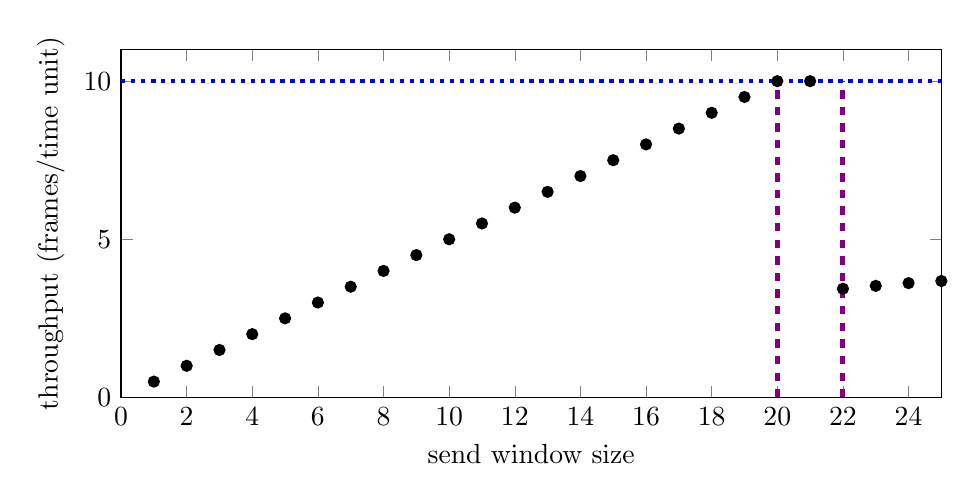
\begin{tikzpicture}
\begin{axis}[width=12cm,height=6cm,
    xlabel=send window size,
    ylabel=throughput (frames/time unit),
    xmin=0,xmax=25,ymin=0]
\addplot[only marks] coordinates {
(1, 0.5000025000125)
(2, 1.0000090000810007)
(3, 1.4999925000374998)
(4, 2.0000280003920055)
(5, 2.500037500562508)
(6, 3.000003000003)
(7, 3.5000035000035)
(8, 4.000048000576006)
(9, 4.499842505512307)
(10, 5.000025000125)
(11, 5.499975250111374)
(12, 5.99977200866367)
(13, 6.499710762871052)
(14, 6.999811005102861)
(15, 7.4996812635462975)
(16, 7.999680012799485)
(17, 8.499426288725509)
(18, 8.999361045365776)
(19, 9.499202067026369)
(20, 9.999100080971061)
(21, 9.999100080973866)
(22, 3.435635094325549)
(23, 3.5274986154570636)
(24, 3.613708966335035)
(25, 3.6808686850100703)
(26, 3.753260645186032)
(27, 3.8487443471573166)
(28, 3.925956461143474)
};
\addplot[blue,dotted,ultra thick,domain=0:25] {10};
    \draw[violet,dashed,ultra thick] (axis cs:20,0) -- (axis cs:20, 10)
     coordinate (empty queue mark);
    \draw[violet,dashed,ultra thick] (axis cs:21.99,0) -- (axis cs:21.99, 10)
     coordinate (full queue mark);
\end{axis}
\end{tikzpicture}
\end{frame}

\begin{frame}[fragile,label=transitTime]{packet transit time}
\begin{tikzpicture}
\draw[ultra thick,arrows={-Latex}] (0, 0) node[left] {sender} -- (1, 0);
\draw[thick] (1, -.5) rectangle (3, .5);
\foreach \x in {2,2.2,2.4,2.6,2.8} {
    \draw (\x, -.5) -- (\x, .5);
}
\node[anchor=south,align=center] at (2, .5) {
    loss when full
};
\node[anchor=north,align=center] at (2, -.5) (queue label) {
    queue
};
\node[anchor=north,font=\fontsize{9}{10}\selectfont] at ([yshift=.3cm]queue label.south) {
    capacity 20
};
\draw[ultra thick,arrows={-Latex}] (3, 0) -- (12, 0) node[right]{receiver}
    node[midway,fill=white,draw=black,very thick,align=left] {
        10 data frames/time unit \\
        1 time unit delay
    }
    node[visible on=<1-3>,ultra thick,pos=0,draw=black,fill=white,font=\tiny,below=.5cm] (data-main) {data};
    \begin{visibleenv}<2->
    \draw[red,-Latex,very thick] (data-main.east) -- (data-main.west -| 13, 0) coordinate (end send)
        node[midway,below,font=\small] {1 time unit (sender to receiver)};
    \end{visibleenv}
\begin{scope}[shift={(12, -4)},x=-1cm]
    \draw[ultra thick,arrows={-Latex}] (0, 0) node[right] {receiver} -- (1, 0);
    \draw[thick] (1, -.5) rectangle (3, .5);
    \foreach \x in {2,2.2,2.4,2.6,2.8} {
        \draw (\x, -.5) -- (\x, .5);
    }
    \node[anchor=south,align=center] at (2, .5) {
        loss when full
    };
    \node[anchor=north,align=center] at (2, -.5) (queue label) {
        queue
    };
    \node[anchor=north,font=\small] at ([yshift=.2cm]queue label.south) {
        capacity 20
    };
    \draw[ultra thick,arrows={-Latex}] (3, 0) -- (12, 0) node[left]{sender}
        node[midway,fill=white,draw=black,very thick,align=left] {
            100 ACK frames/time unit \\
            1 time unit delay
        }
        node[visible on=<2->,pos=0,draw=red,fill=white,font=\tiny,below=.5cm,align=center,inner sep=0.5mm] 
            (ack-start) {a\\c\\k};
    \begin{visibleenv}<2->
        \draw[dotted,red,-Latex,very thick] (end send) |- (ack-start.east);
        \draw[red,-Latex,very thick] (ack-start.west) -- (ack-start.west -| 12, 0) node[midway,below,font=\small] { + 1 time unit (receiver to sender)};
    \end{visibleenv}
\end{scope}
\begin{visibleenv}<3>
\node[draw=red,fill=white,ultra thick,align=left] at (6, -2.5) {
    takes 1 + 1 time units to send message + receive ack \\
    goal: keep sending stuff while waiting
};
\end{visibleenv}
\end{tikzpicture}
\end{frame}

\begin{frame}{filling the pipe}
    \begin{itemize}
    \item round-trip time of 2 time units
        \begin{itemize}
        \item from send data to receive ACK (assuming no queuing delay)
        \end{itemize}
    \item can send 10 data frames per time unit
    \item = can send 20 data frames while waiting for ACK
    \vspace{.5cm}
    \item<2> \myemph{``bandwidth-delay product''}
        \begin{itemize}
        \item 10/time unit (banwidth) times 2 time unit (RTT = delay)
        \end{itemize}
    \end{itemize}
\end{frame}

\begin{frame}[fragile,label=throughAndWindow]{throughput and window size (detail)}
\begin{tikzpicture}
\begin{axis}[width=12cm,height=6cm,
    xlabel=send window size,
    ylabel=throughput (frames/time unit),
    xmin=17,xmax=24,ymin=0]
\addplot[only marks] coordinates {
(1, 0.5000025000125)
(2, 1.0000090000810007)
(3, 1.4999925000374998)
(4, 2.0000280003920055)
(5, 2.500037500562508)
(6, 3.000003000003)
(7, 3.5000035000035)
(8, 4.000048000576006)
(9, 4.499842505512307)
(10, 5.000025000125)
(11, 5.499975250111374)
(12, 5.99977200866367)
(13, 6.499710762871052)
(14, 6.999811005102861)
(15, 7.4996812635462975)
(16, 7.999680012799485)
(17, 8.499426288725509)
(18, 8.999361045365776)
(19, 9.499202067026369)
(20, 9.999100080971061)
(21, 9.999100080973866)
(22, 3.435635094325549)
(23, 3.5274986154570636)
(24, 3.613708966335035)
(25, 3.6808686850100703)
(26, 3.753260645186032)
(27, 3.8487443471573166)
(28, 3.925956461143474)
};
\addplot[blue,dotted,ultra thick,domain=0:25] {10};
    \draw[violet,dashed,ultra thick] (axis cs:20,0) -- (axis cs:20, 11)
     coordinate (empty queue mark);
    \draw[violet,dashed,ultra thick] (axis cs:21.99,0) -- (axis cs:21.99, 11)
     coordinate (full queue mark);
\end{axis}
\node[violet,anchor=south east,align=right] (nq) at ([xshift=1.5cm]empty queue mark) {
    (no queuing delay)
};
\node[violet,anchor=south west,align=left] (mq) at ([xshift=-1.5cm]full queue mark) {
    (max queuing delay)
};
\node[violet,anchor=south] at ($(nq)!0.5!(mq)$) {bandwidth-delay product};
\end{tikzpicture}
\end{frame}


\begin{frame}[fragile,label=fullPipe]{filling the pipe}
\begin{tikzpicture}
\draw[ultra thick,arrows={-Latex}] (0, 0) node[left] {sender} -- (1, 0);
\draw[thick] (1, -.5) rectangle (3, .5);
\foreach \x in {2,2.2,2.4,2.6,2.8} {
    \draw (\x, -.5) -- (\x, .5);
}
\node[anchor=south,align=center] at (2, .5) {
    loss when full
};
\node[anchor=north,align=center] at (2, -.5) (queue label) {
    queue
};
\node[anchor=north,font=\fontsize{9}{10}\selectfont] at ([yshift=.3cm]queue label.south) {
    capacity 20
};
\draw[ultra thick,arrows={-Latex}] (3, 0) -- (12, 0) node[right]{receiver}
    node[midway,fill=white,draw=black,very thick,align=left] {
        10 data frames/time unit \\
        1 time unit delay
    }
    \foreach \x in {0,1,2,3,4,5,6,7,8,9} {
        node[visible on=<3->,pos=\x*.1+0.05,draw=black,fill=white,font=\tiny,below=.5cm] (data-\x) {data}
    };
    \begin{visibleenv}<3->
    \draw[red,Latex-Latex] ([yshift=-.1cm]data-0.south west) -- ([yshift=-.1cm]data-1.south west)
        node[below,font=\small] {0.1 time unit};
    \end{visibleenv}
\begin{scope}[shift={(12, -4)},x=-1cm]
    \draw[ultra thick,arrows={-Latex}] (0, 0) node[right] {receiver} -- (1, 0);
    \draw[thick] (1, -.5) rectangle (3, .5);
    \foreach \x in {2,2.2,2.4,2.6,2.8} {
        \draw (\x, -.5) -- (\x, .5);
    }
    \node[anchor=south,align=center] at (2, .5) {
        loss when full
    };
    \node[anchor=north,align=center] at (2, -.5) (queue label) {
        queue
    };
    \node[anchor=north,font=\small] at ([yshift=.2cm]queue label.south) {
        capacity 20
    };
    \draw[ultra thick,arrows={-Latex}] (3, 0) -- (12, 0) node[left]{sender}
        node[midway,fill=white,draw=black,very thick,align=left] {
            100 ACK frames/time unit \\
            1 time unit delay
        }
        \foreach \x in {0,1,2,3,4,5,6,7,8,9} {
            node[visible on=<3->,pos=\x*.1+0.05,draw=black,fill=white,font=\tiny,below=.5cm,align=center,inner sep=0.5mm] {a\\c\\k}
        };
\end{scope}
\end{tikzpicture}
\end{frame}



\begin{frame}[fragile,label=throughAndWindow]{throughput and window size (detail)}
\begin{tikzpicture}
\begin{axis}[width=12cm,height=6cm,
    xlabel=send window size,
    ylabel=throughput (frames/time unit),
    xmin=17,xmax=24,ymin=0]
\addplot[only marks] coordinates {
(1, 0.5000025000125)
(2, 1.0000090000810007)
(3, 1.4999925000374998)
(4, 2.0000280003920055)
(5, 2.500037500562508)
(6, 3.000003000003)
(7, 3.5000035000035)
(8, 4.000048000576006)
(9, 4.499842505512307)
(10, 5.000025000125)
(11, 5.499975250111374)
(12, 5.99977200866367)
(13, 6.499710762871052)
(14, 6.999811005102861)
(15, 7.4996812635462975)
(16, 7.999680012799485)
(17, 8.499426288725509)
(18, 8.999361045365776)
(19, 9.499202067026369)
(20, 9.999100080971061)
(21, 9.999100080973866)
(22, 3.435635094325549)
(23, 3.5274986154570636)
(24, 3.613708966335035)
(25, 3.6808686850100703)
(26, 3.753260645186032)
(27, 3.8487443471573166)
(28, 3.925956461143474)
};
\addplot[blue,dotted,ultra thick,domain=0:25] {10};
    \draw[violet,dashed,ultra thick] (axis cs:20,0) -- (axis cs:20, 11)
     coordinate (empty queue mark);
    %\draw[violet,dashed,ultra thick] (axis cs:21.99,0) -- (axis cs:21.99, 11)
    % coordinate (full queue mark);
\end{axis}
\node[violet,anchor=south east,align=right] (nq) at ([xshift=1.5cm]empty queue mark) {
    (no queuing delay)
};
\node[violet,anchor=south west,align=left] (mq) at ([xshift=-1.5cm]full queue mark) {
    (max useful queuing delay)
};
\node[violet,anchor=south] at (nq) {bandwidth-delay product\\w/o queuing delay};
\end{tikzpicture}
\end{frame}


\begin{frame}[fragile,label=fullPipe]{filling the pipe}
\begin{tikzpicture}
\draw[ultra thick,arrows={-Latex}] (0, 0) node[left] {sender} -- (1, 0);
\draw[thick] (1, -.5) rectangle (3, .5);
\foreach \x in {2,2.2,2.4,2.6,2.8} {
    \draw (\x, -.5) -- (\x, .5);
}
\node[anchor=south,align=center] at (2, .5) {
    loss when full
};
\node[anchor=north,align=center] at (2, -.5) (queue label) {
    queue
};
\node[anchor=north,font=\fontsize{9}{10}\selectfont] at ([yshift=.3cm]queue label.south) {
    capacity 20
};
\draw[ultra thick,arrows={-Latex}] (3, 0) -- (12, 0) node[right]{receiver}
    node[midway,fill=white,draw=black,very thick,align=left] {
        10 data frames/time unit \\
        1 time unit delay
    }
    \foreach \x in {0,1,2,3,4,5,6,7,8,9} {
        node[visible on=<3->,pos=\x*.1+0.05,draw=black,fill=white,font=\tiny,below=.5cm] (data-\x) {data}
    };
    \begin{visibleenv}<3->
    \draw[red,Latex-Latex] ([yshift=-.1cm]data-0.south west) -- ([yshift=-.1cm]data-1.south west)
        node[below,font=\small] {0.1 time unit};
    \end{visibleenv}
\begin{scope}[shift={(12, -4)},x=-1cm]
    \draw[ultra thick,arrows={-Latex}] (0, 0) node[right] {receiver} -- (1, 0);
    \draw[thick] (1, -.5) rectangle (3, .5);
    \foreach \x in {2,2.2,2.4,2.6,2.8} {
        \draw (\x, -.5) -- (\x, .5);
    }
    \node[anchor=south,align=center] at (2, .5) {
        loss when full
    };
    \node[anchor=north,align=center] at (2, -.5) (queue label) {
        queue
    };
    \node[anchor=north,font=\small] at ([yshift=.2cm]queue label.south) {
        capacity 20
    };
    \draw[ultra thick,arrows={-Latex}] (3, 0) -- (12, 0) node[left]{sender}
        node[midway,fill=white,draw=black,very thick,align=left] {
            100 ACK frames/time unit \\
            1 time unit delay
        }
        \foreach \x in {0,1,2,3,4,5,6,7,8,9} {
            node[visible on=<3->,pos=\x*.1+0.05,draw=black,fill=white,font=\tiny,below=.5cm,align=center,inner sep=0.5mm] {a\\c\\k}
        };
\end{scope}
\end{tikzpicture}
\end{frame}

\begin{frame}{on bursts}
    \begin{itemize}
    \item max possible queuing delay suggests window size of 30
        \begin{itemize}
        \item approx. 3 time units times 10
        \end{itemize}
    \item problem: ``bursts'' temporarily exceed queue size
    \vspace{.5cm}
    \item achievable average queue size not that high
    \item sender could moderate by ``pacing'' packets
    \end{itemize}
\end{frame}


\subsection{problems solved}
\begin{frame}{sliding windows solve\ldots}
    \begin{itemize}
    \item reliability on unrelaible link
    \item \textit{congestion control}
        \begin{itemize}
        \item keep network from being overloaded
        \item \ldots by having window sizes set correctly
        \end{itemize}
    \item \textit{flow control}
        \begin{itemize}
        \item keep sender from getting too far ahead of sender
        \item \ldots by having window sizes set correctly
        \end{itemize}
    \end{itemize}
\end{frame}


\subsection{sequence number wraparound}
\usetikzlibrary{arrows.meta, calc, fit, matrix, patterns, shapes.misc}

\providecommand{\computer}{%
    
\includegraphics[width=1cm]{../common/Noun_project_216.pdf}
}
\providecommand{\switch}{%
    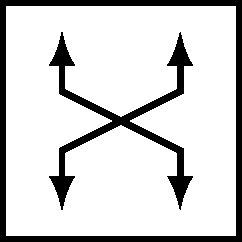
\includegraphics[width=0.9cm]{../common/fig-switch.pdf}
}
\providecommand{\bigswitch}{%
    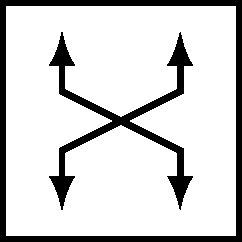
\includegraphics[width=1.4cm]{../common/fig-switch.pdf}
}
\providecommand{\router}{%
    
\includegraphics[width=0.9cm]{../common/fig-router.pdf}
}


\begin{frame}{sequence number wraparound}
    \begin{itemize}
    \item protocol so far requires arbitrarily large sequence numbers
        \begin{itemize}
        \item doing $<$ and $>$ checks on sequence number, so they need to increase
        \end{itemize}
    \item would like to use smaller sequence numbers
        \begin{itemize}
        \item think: transferring multi-gigabyte file
        \end{itemize}
    \item question: what goes wrong when we reuse sequeunce numbers?
    \end{itemize}
\end{frame}

\begin{frame}{sender/receiver desync: missing ACKs}
\begin{tikzpicture}
\tikzset{
    seqlist/.style={tight matrix,nodes={text width=.8cm,minimum height=.8cm},column sep=.6mm},
    dots/.style={draw=none,execute at begin node=\ldots,anchor=center,font=\huge,text width=1cm,align=center},
    region mark/.style={very thick,decorate,decoration={brace,mirror}},
    region mark label/.style={midway,below,align=center},
    verified/.style={pattern color=black!30,pattern=checkerboard},
    ack sent not recvd/.style={fill=blue!60},
    unsent ready/.style={pattern color=yellow!30!black,pattern=checkerboard},
    unsent/.style={pattern=crosshatch dots,pattern color=violet!70},
}
\begin{scope}[name prefix=s-]
    \matrix[seqlist] (window) {
        |[dots,alias=window-start]| ~ \& |[alias=after-window-start,verified,alias=LAR]| ~ \&
        |[ack sent not recvd,alias=after LAR]| ~ \& |[ack sent not recvd]| ~ \& |[ack sent not recvd]| ~ \& 
        |[ack sent not recvd,alias=LFS]| ~ \& 
        |[alias=after LFS,unsent]| ~ \& |[unsent,alias=before-window-end]| ~  \&
        |[unsent]| ~  \&
        |[unsent]| ~  \&
        |[unsent]| ~  \&
        |[unsent,alias=before-window-end]| ~  \&
        \& |[alias=window-end,dots]| \\
    };
    \node[anchor=east] at (window-start.west) {sender};
    \draw[thick,Latex-] (LAR.north) -- ++(0,.5) node[above,align=center] (LAR label) {(LAR)\\last ACK recv'd};
    \draw[thick,Latex-] (LFS.north) -- ++(0,.5) node[above,align=center] (LFS label) {(LFS)\\last frame sent};
\end{scope}
\begin{scope}[name prefix=r-,yshift=-3cm]
    \matrix[seqlist] (window) {
        |[dots,alias=window-start]| ~ \& |[alias=after-window-start,verified]| ~ \& 
        |[alias=after LAR,ack sent not recvd]| ~ \& |[ack sent not recvd]| ~ \& 
        |[ack sent not recvd]| ~ \& |[alias=LFR,ack sent not recvd]| ~ \&
        |[unsent ready,alias=after LFR]| ~ \& |[unsent ready,alias=after after LFR]| ~ \&
        |[unsent ready]| ~ \& |[unsent ready,alias=LAF]| ~ \& 
        |[alias=after LAF,unsent]| ~ \& |[unsent,alias=before-window-end]| ~ \& |[alias=window-end,dots]| \\
    };
    \node[anchor=east] at (window-start.west) {receiver};
    \draw[thick,Latex-] (LFR.north) -- ++(0,.5) node[above,align=center] {(LFR)\\last frame recv'd*};
    \draw[thick,Latex-] (LAF.north) -- ++(0,.5) node[above,align=center] {(LAF)\\last accepted frame};
    \draw[region mark] ([yshift=-.1cm]after LAR.south west) -- ([yshift=-.1cm]LFR.south east)
        node[region mark label] {resent if \\ ACK lost};
    \draw[region mark] ([yshift=-.1cm]after LFR.south west) -- ([yshift=-.1cm]LAF.south east)
        node[region mark label] {expected if \\ ACK not lost};
\end{scope}
\begin{visibleenv}<2->
\node[draw=red,ultra thick,fit=(s-after LAR) (r-LAF),label={[red,align=left,fill=white,fill opacity=0.95]west:need unique \\ numbers for all these}] {};
\end{visibleenv}
\begin{visibleenv}<3->
\foreach \x/\lbl in {2/4,3/5,4/6,5/7,6/0,7/1,8/2,9/3,10/4,11/5,12/6,13/7} {
    \node[fill=white,font=\small,text=red,circle,draw=red,ultra thick,anchor=south west,inner sep=0.1mm] at ([xshift=\x * .935cm - 0.4cm]s-window-start.north west) {\lbl};
}
\end{visibleenv}
\end{tikzpicture}
\end{frame}

\begin{frame}{wraparound}
\begin{tikzpicture}
\tikzset{
    box/.style={thick},
    message/.style={draw,thick,-Latex},
    failure/.style={draw,ultra thick,red,cross out,minimum width=1cm,minimum height=1cm},
    every node/.style={inner sep=0.1mm},
}
\begin{scope}[xshift=1cm,x=0.9cm,y=0.9cm]
\draw[box] (0, 0) rectangle ++(2, -8) 
    node[midway,align=center] {machine\\A};
\draw[box] (13, 0) rectangle ++(2, -8) 
    node[midway,align=center] {machine\\B};
\draw[message] (2, -0.5) -- (13, -1.5) node[pos=0.25,above,sloped] {\myemph{0}: ``The ''};
\draw[message] (13, -1.75) -- (2, -2.75) node[pos=0.25,sloped,below] {got up to \myemph{0}};
\draw[message] (2, -1) -- (13, -2) node[pos=0.25, above, sloped] {\myemph{1}: ``meeting''};
\draw[message] (13, -2.25) -- (2, -3.25) node[pos=0.25, sloped,below] {got up to \myemph{1}};

% in response to got 0
\draw[message] (2, -3) -- (13, -4) node[pos=0.5, above, sloped] {\myemph{2}: ``is''};
\draw[message] (13, -4.25) -- (2, -5.25) node[pos=0.25, sloped,below] {got up to \myemph{2}};
% in response to got 1
\draw[message] (2, -3.5) -- (13, -4.5) node[pos=0.5, above, sloped] {\myemph{3}: ``at''};
\draw[message] (13, -4.75) -- (2, -5.75) node[pos=0.25, sloped,below] {got up to \myemph{3}};

% in response to got 2
\draw[message] (2, -5.5) -- (13, -6.5) node[pos=0.5, above, sloped] {\myemph{0}: ``12pm''};
\draw[message] (13, -6.75) -- (2, -7.75) node[pos=0.25, sloped,below] {got up to \myemph{0}};
\end{scope}
\end{tikzpicture}
\end{frame}

\begin{frame}{loss and resend?}
\begin{tikzpicture}
\tikzset{
    box/.style={thick},
    message/.style={draw,thick,-Latex,font=\small},
    failure/.style={draw,ultra thick,red,cross out,minimum width=1cm,minimum height=1cm},
    every node/.style={inner sep=0.1mm},
}
\begin{scope}[xshift=1cm,x=0.9cm,y=0.7cm]
\draw[box] (0, 2) rectangle ++(2, -10) 
    node[midway,align=center] {machine\\A};
\draw[box] (13, 2) rectangle ++(2, -10) 
    node[midway,align=center] {machine\\B};
\draw[message] (2, 2-0.5) -- (9, 2-1.2) node[pos=0.25,above,sloped] {\myemph{0}: ``The ''} node[failure] {};
\draw[message] (2, 2-1) -- (9, 2-1.8) node[pos=0.25, above, sloped] {\myemph{1}: ``meeting''} node[failure] {};
\draw[message] (13, -2.25) -- (2, -3.25) node[pos=0.25, sloped,below] {got up to \myemph{1}};
\draw[message] (2, -0.5) -- (13, -1.5) node[pos=0.25,above,sloped] {\myemph{0}: ``The ''};
\draw[message] (13, -1.75) -- (2, -2.75) node[pos=0.25,sloped,below] {got up to \myemph{0}};
\draw[message] (2, -1) -- (13, -2) node[pos=0.25, above, sloped] {\myemph{1}: ``meeting''};
\draw[message] (13, -2.25) -- (2, -3.25) node[pos=0.25, sloped,below] {got up to \myemph{1}};

% in response to got 0
\draw[message] (2, -3) -- (13, -4) node[pos=0.5, above, sloped] {\myemph{2}: ``is''};
\draw[message] (13, -4.25) -- (2, -5.25) node[pos=0.25, sloped,below] {got up to \myemph{2}};
% in response to got 1
\draw[message] (2, -3.5) -- (13, -4.5) node[pos=0.5, above, sloped] {\myemph{3}: ``at''};
\draw[message] (13, -4.75) -- (2, -5.75) node[pos=0.25, sloped,below] {got up to \myemph{3}};

% in response to got 2
\draw[message] (2, -5.5) -- (13, -6.5) node[pos=0.5, above, sloped] {\myemph{0}: ``12pm''};
\draw[message] (13, -6.75) -- (2, -7.75) node[pos=0.25, sloped,below] {got up to \myemph{0}};
\end{scope}
\end{tikzpicture}
\end{frame}

\begin{frame}{very bad reordering}
\begin{tikzpicture}
\tikzset{
    box/.style={thick},
    message/.style={draw,thick,-Latex,font=\small},
    failure/.style={draw,ultra thick,red,cross out,minimum width=1cm,minimum height=1cm},
    every node/.style={inner sep=0.1mm},
}
\begin{scope}[xshift=1cm,x=0.9cm,y=0.7cm]
\draw[box] (0, 2) rectangle ++(2, -10) 
    node[midway,align=center] {machine\\A};
\draw[box] (13, 2) rectangle ++(2, -10) 
    node[midway,align=center] {machine\\B};
\draw[message] (2, 2-0.5) -- (13, -6) node[pos=0.1,above,sloped,font=\bfseries] {\myemph{0}: ``The ''};
\draw[message] (2, 2-1) -- (9, 2-1.8) node[pos=0.75, above, sloped] {\myemph{1}: ``meeting''} node[failure] {};
\draw[message] (13, -2.25) -- (2, -3.25) node[pos=0.25, sloped,below] {got up to \myemph{1}};
\draw[message] (2, -0.5) -- (13, -1.5) node[pos=0.25,above,sloped] {\myemph{0}: ``The ''};
\draw[message] (13, -1.75) -- (2, -2.75) node[pos=0.25,sloped,below] {got up to \myemph{0}};
\draw[message] (2, -1) -- (13, -2) node[pos=0.25, above, sloped] {\myemph{1}: ``meeting''};
\draw[message] (13, -2.25) -- (2, -3.25) node[pos=0.25, sloped,below] {got up to \myemph{1}};

% in response to got 0
\draw[message] (2, -3) -- (13, -4) node[pos=0.5, above, sloped] {\myemph{2}: ``is''};
\draw[message] (13, -4.25) -- (2, -5.25) node[pos=0.25, sloped,below] {got up to \myemph{2}};
% in response to got 1
\draw[message] (2, -3.5) -- (13, -4.5) node[pos=0.5, above, sloped] {\myemph{3}: ``at''};
\draw[message] (13, -4.75) -- (2, -5.75) node[pos=0.25, sloped,below] {got up to \myemph{3}};

% in response to got 2
\draw[message] (2, -5.5) -- (13, -6.5) node[pos=0.5, above, sloped,font=\bfseries] {\myemph{0}: ``12pm''};
% in response to BOGUS got 0
\draw[message] (13, -6.25) -- (2, -7.25) node[pos=0.25, sloped,below] {got up to \myemph{0}};
\end{scope}
\end{tikzpicture}
\end{frame}

\begin{frame}{possible reason}
\begin{tikzpicture}
\tikzset{
    connect one/.style={draw,very thick,Latex-Latex},
    computer/.style={inner sep=0mm,outer sep=0mm,execute at begin node={\computer}},
    switch/.style={inner sep=0mm,outer sep=0mm,execute at begin node={\switch}},
    router/.style={inner sep=0mm,outer sep=0mm,execute at begin node={\router}},
    big switch/.style={inner sep=0mm,outer sep=0mm,execute at begin node={\bigswitch}},
    packet/.style={minimum width=.4cm,minimum height=0.2cm,inner sep=0mm,outer sep=0mm,draw},
    packet lg/.style={minimum width=.6cm,minimum height=0.2cm,inner sep=0mm,outer sep=0mm,draw},
}
\node[computer] (start) at (0,0) {};
\node[computer] (end)  at (13,0) {};
\node[router] (pre1) at (3, 3) {};
\node[router] (pre2) at (4, .5) {};
\node[router] (pre3) at (5, 3) {};
\node[router] (A) at (6, 1) {};
\node[router] (B) at (7, -1) {};
\node[router] (C) at (8, 3) {};
\node[router] (D) at (11, 0) {};
\
\node[router] (E) at (7.5, -2) {};
\foreach \x/\y in {start/pre1,pre1/pre2,pre2/pre3,pre3/A,A/B,B/C,C/D,D/end,start/E,E/end} {
    \draw[connect one] (\x) -- (\y);
}
\node[font=\small,draw,fill=white] at ($(C)!0.5!(D)$) {\myemph{0}: ``The ''};
\node[font=\small,draw,fill=white] at ($(E)!0.7!(start)$) {\myemph{0}: ``12pm''};
\end{tikzpicture}
\end{frame}





\section{TCP example}

\subsection{TCP segment format}
\usetikzlibrary{patterns}
\begin{frame}{TCP}
    \begin{itemize}
    \item transmission control protocol (TCP)
    \item implements reliable streams of bytes
    \item similar mechanism to what we've described
    \end{itemize}
\end{frame}

\begin{frame}{TCP extras/differences}
    \begin{itemize}
    \item bidirectional ---
        \begin{itemize}
        \item separate sequence numbers in each direction
        \item can combine data (from A to B) with acknowledgment (from B to A)
        \end{itemize}
    \item sequence numbers are byte numbers ---
        \begin{itemize}
        \item can retransmit data in different sized packets
        \item sequence numbers = index of \textit{first byte} sent
        \item acknowledgment numbers = index of \textit{last byte} acknowledged
        \end{itemize}
    \item dynamic/variable window sizes
        \begin{itemize}
        \item we'll discuss strategies later
        \end{itemize}
    \item offical name for packets = \textit{segments}
    \end{itemize}
\end{frame}

\begin{frame}[fragile]{TCP segment format}
\begin{tikzpicture}
    \tikzset{
        box/.style={draw,thick},
        box unused/.style={draw,thick,pattern=north west lines},
        box label/.style={midway,font=\small,align=center},
        box label flags/.style={midway,font=\fontsize{8}{9}\selectfont,align=center},
        hi on/.style={alt=<#1>{ultra thick,fill=red!10}},
        explain box 1/.style={draw=red,line width=0.8mm,fill=white,anchor=center,at={(explain box loc 1)},align=center},
        explain box 2/.style={draw=red,line width=0.8mm,fill=white,anchor=center,at={(explain box loc 2)},align=center},
        explain box 3/.style={draw=red,line width=0.8mm,fill=white,anchor=center,at={(explain box loc 3)},align=center},
    }
    \begin{scope}[x=4.7mm,y=9mm]
        \coordinate (explain box loc 1) at (16, -3.1);
        \coordinate (explain box loc 2) at (16, -5.1);
        \coordinate (explain box loc 3) at (16, -1.1);
        \path[shading=axis,top color=white,bottom color=black!20] (0, 1) rectangle (32, 0)
            node[box label] {(lower layer header)};
        \path[box,hi on=2] (0, 0) rectangle (16, -1) node[box label] {source port (16b)};
        \path[box,hi on=2] (16, 0) rectangle (32, -1) node[box label] {destination port (16b)};
        \path[box,hi on=3] (0, -1) rectangle (32, -2) node[box label] {sequence number (32b)};
        \path[box,hi on=4] (0, -2) rectangle (32, -3) node[box label] {acknowledgment number (32b)};
        \path[box,hi on=10] (0, -3) rectangle (4, -4) node[box label] {data offset\\(4b)};
        \path[box unused] (4, -3) rectangle (8, -4);
        \path[box,hi on=9] (8, -3) rectangle ++(1, -1) node[box label flags]{C\\W\\R};
        \path[box,hi on=9] (9, -3) rectangle ++(1, -1) node[box label flags]{E\\C\\E};
        \path[box,hi on=6] (10, -3) rectangle ++(1, -1) node[box label flags]{U\\R\\G};
        \path[box,hi on=4] (11, -3) rectangle ++(1, -1) node[box label flags]{A\\C\\K};
        \path[box,hi on=7] (12, -3) rectangle ++(1, -1) node[box label flags]{P\\S\\H};
        \path[box,hi on=8] (13, -3) rectangle ++(1, -1) node[box label flags]{R\\S\\T};
        \path[box,hi on=8] (14, -3) rectangle ++(1, -1) node[box label flags]{S\\Y\\N};
        \path[box,hi on=8] (15, -3) rectangle ++(1, -1) node[box label flags]{F\\I\\N};
        \path[box,hi on=5] (16, -3) rectangle ++(16, -1) node[box label] {window size (16b)};
        \path[box] (0, -4) rectangle ++(16, -1) node[box label] {checksum (16b)};
        \path[box, hi on=6] (16, -4) rectangle ++(16, -1) node[box label] {urgent pointer (16b)};
        \path[box,hi on=10] (0, -5) rectangle ++(32, -1) node[box label] {options (variable)};
        \draw[line width=1mm,white] (-.2, -5.55) -- (.2, -5.45);
        \draw[line width=1mm,white] (32 -.2, -5.55) -- (32 + .2, -5.45);
        \draw[very thick,black] (-.2, -5.5) -- (.2, -5.4);
        \draw[very thick,black] (32 -.2, -5.5) -- (32 + .2, -5.4);
        \draw[very thick,black] (-.2, -5.6) -- (.2, -5.5);
        \draw[very thick,black] (32 -.2, -5.6) -- (32 + .2, -5.5);
        \path[overlay,shading=axis,top color=black!20,bottom color=white] (0, -6) rectangle (32, -7)
            node[box label] {(data)};
    \end{scope}
    \begin{visibleenv}<2>
        \node[explain box 1] {
            ports identify program/socket on machines \\
            (we'll talk more when we cover sockets) \\
            ~ \\
            machines identified in lower layer headers 
        };
    \end{visibleenv}
    \begin{visibleenv}<3>
        \node[explain box 2] {
            byte number for first byte of data in this packet
        };
    \end{visibleenv}
    \begin{visibleenv}<4>
        \node[explain box 2] {
            ack number = byte number of largest byte acknowledged \\
            only meaningful if ACK `flag' is 1
        };
    \end{visibleenv}
    \begin{visibleenv}<5>
        \node[explain box 3] {
            window size is receive window size \\
            tells sender how much receiver will accept \\
            sender window could/often will be different \\
            (and not directly visible in packets)
        };
    \end{visibleenv}
    \begin{visibleenv}<6>
        \node[explain box 3] {
            some fields related to `urgent data' mechanism \\
            almost never used today
        };
    \end{visibleenv}
    \begin{visibleenv}<7>
        \node[explain box 3] {
            PSH (push) `flag' is hint that sender does not have \\
            more data to send right away
        };
    \end{visibleenv}
    \begin{visibleenv}<8>
        \node[explain box 3] {
            RST (reset), SYN (synchornize), FIN flags \\
            used for connnection management \\
            (we'll talk more when we cover sockets)
        };
    \end{visibleenv}
    \begin{visibleenv}<9>
        \node[explain box 3] {
            CWR (congestion window reduced) and \\
            ECE (explicit congestion notification echo) flags \\
            sometimes used as part of setting window size \\
            to match network conditions (later topic for us)
        };
    \end{visibleenv}
    \begin{visibleenv}<10>
        \node[explain box 3] {
            header can have variable number of ``options'' \\
            technically optional, almost always used today \\
            ~ \\
            size of header indicated by \textit{data offset} \\
            (data offset is units of 32-bit words, not bytes)
        };
    \end{visibleenv}
\end{tikzpicture}
\end{frame}

\begin{frame}{exercise: maximum throughput}
    \begin{itemize}
    \item let's say we have a receiver window size of 65535 bytes
    \item and a round-trip time of 100 ms
    \vspace{.5cm}
    \item if we want to avoid sending data the sender will reject as outside
    its window, maximum throughput?
    \end{itemize}
\begin{tabular}{ll}
A. around 32kbyte/sec &
B. around 64kbyte/sec \\
C. around 128kbyte/sec &
D. around 320kbyte/sec \\
E. around 640kbyte/sec &
F. around 1280kbyte/sec \\
G. something else \\
\end{tabular}
\end{frame}

\begin{frame}{selected TCP options}
    \begin{itemize}
    \item window size scale factor
        \begin{itemize}
        \item allow receiver window sizes greater than 64k
        \item needed to get reasonable bandwidth on modern networks
        \end{itemize}
    \item timestamps
        \begin{itemize}
        \item allow figuring out round trip time to estimate timeout
        \item extend 32-bit sequence number, which is too small for multi-gigabit networks
        \end{itemize}
    \item selective acknowledgements
        \begin{itemize}
        \item allow providing information about `holes' in received data
        \item example: I got bytes 1--5000, 6000--7000, 8000--9000
        \item without it would only say 5000
        \end{itemize}
    \end{itemize}
\end{frame}

\begin{frame}[fragile]{selected TCP option formats}
\begin{tikzpicture}
    \tikzset{
        box/.style={draw,thick},
        box unused/.style={draw,thick,pattern=north west lines},
        box label/.style={midway,font=\small,align=center},
        box label flags/.style={midway,font=\fontsize{8}{9}\selectfont,align=center},
        hi on/.style={alt=<#1>{ultra thick,fill=red!10}},
        explain box 1/.style={draw=red,line width=0.8mm,fill=white,anchor=center,at={(explain box loc 1)},align=center},
        explain box 2/.style={draw=red,line width=0.8mm,fill=white,anchor=center,at={(explain box loc 2)},align=center},
        explain box 3/.style={draw=red,line width=0.8mm,fill=white,anchor=center,at={(explain box loc 3)},align=center},
    }
    \begin{scope}[x=4.7mm,y=9mm]
        \coordinate (explain box loc 1) at (16, -5.1);
        \coordinate (explain box loc 2) at (16, -6.1);
        \coordinate (explain box loc 3) at (16, -1.1);
        \path[box,hi on=3] (0, 0) rectangle (8, -1) node[box label] {kind (8b)};
        \path[box,hi on=2] (8, 0) rectangle (16, -1) node[box label] {length (8b)};
        \path[shading=axis,left color=black!20,right color=white] (16, 0) rectangle (32, -1) node[box label] {option data};

        \node[anchor=south] at (16, -2) {\myemph<4>{window scale option}:};
        \path[box,hi on=4,hi on=3] (0, -2) rectangle ++(8, -1) node[box label] {\tt 3};
        \path[box,hi on=2,hi on=4] (8, -2) rectangle ++(8, -1) node[box label] {\tt 3};
        \path[box,hi on=4] (16, -2) rectangle ++(8, -1) node[box label] {shift count};
        
        \node[anchor=south] at (16, -4) {\myemph<5>{timestamps}:};
        \path[box,hi on=3] (0, -4) rectangle ++(8, -1) node[box label] {\tt 8};
        \path[box,hi on=2] (8, -4) rectangle ++(8, -1) node[box label] {\tt 10};
        \path[box] (16, -4) rectangle ++(16, -1) node[box label] {sender TS};
        \path[box,hi on=6] (0, -5) rectangle ++(16, -1) node[box label] {echoed TS};
    \end{scope}
    \begin{visibleenv}<2>
        \node[explain box 2] {
            length field permits skipping unrecognized options
        };
    \end{visibleenv}
    \begin{visibleenv}<3>
        \node[explain box 2] {
            unique kind codes for each option \\
            list of valid codes maintained by IANA \\
            (Internet Assigned Numbers Authority) 
        };
    \end{visibleenv}
    \begin{visibleenv}<4>
        \node[explain box 1] {
            sent only in connection setup \\
            only takes effect if both sides send it \\
            sets amount to left-shift \\
            all window size fields by
        };
    \end{visibleenv}
    \begin{visibleenv}<6>
        \node[explain box 3] {
            echoed timestamp --- \\
            only valid in ACK messages \\
            copy of timestamp sent in message ACK'd \\
            allows computing round-trip-time
        };
    \end{visibleenv}
\end{tikzpicture}
\end{frame}



%\subsection{TCP connection example 1}
%\begin{frame}{a TCP connection}
\begin{tikzpicture}
\tikzset{
    overlay box/.style={fill=white,fill opacity=0.9},
}
\node[overlay,anchor=north west,inner sep=0mm] (base) at (0, 0) {%
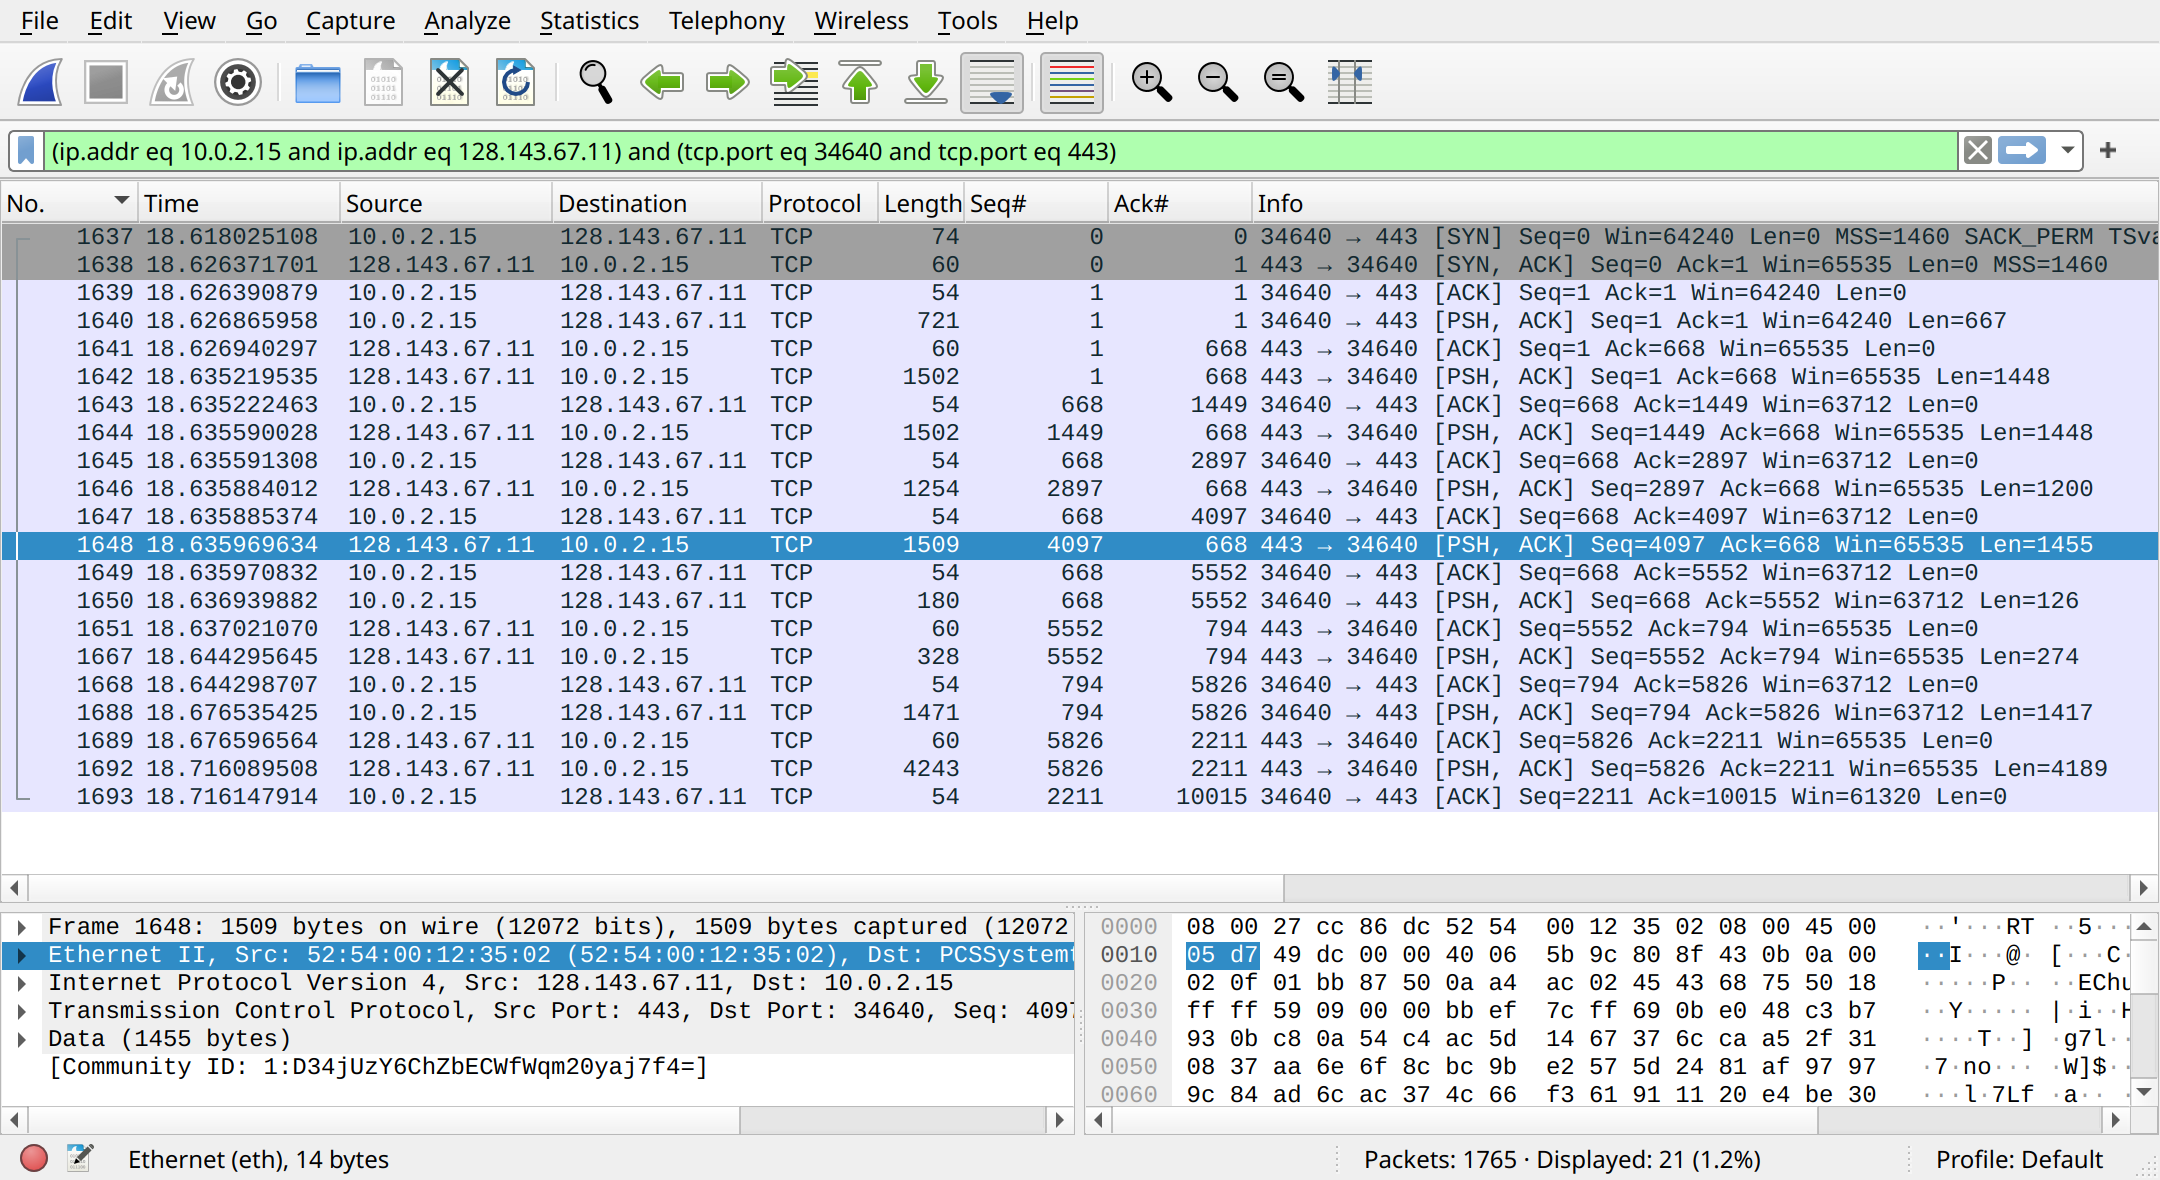
\includegraphics[width=\textwidth]{../reliable/wireshark-tcp-ex1-over}%
};
\path (0, 0) rectangle (14.5, -7); % for bounding box
\draw[overlay,help lines] (0, 0) grid (14, -8);
\begin{visibleenv}<2>

\end{visibleenv}
\end{tikzpicture}
\end{frame}


\subsection{TCP connection example}
\usetikzlibrary{shapes.geometric,spy}
\begin{frame}[fragile]{a TCP connection}
\tikzset{
    overlay box/.style={fill=white,fill opacity=0.95},
}
\begin{tikzpicture}[
    spy using outlines={%
        overlay,circle,magnification=2,size=2cm,connect spies,%
        every spy on node/.append style={very thick},%
        ultra thick,%
    }
]
\node[overlay,anchor=north west,inner sep=0mm] (base) at (0, 0) {%
\only<1-2>{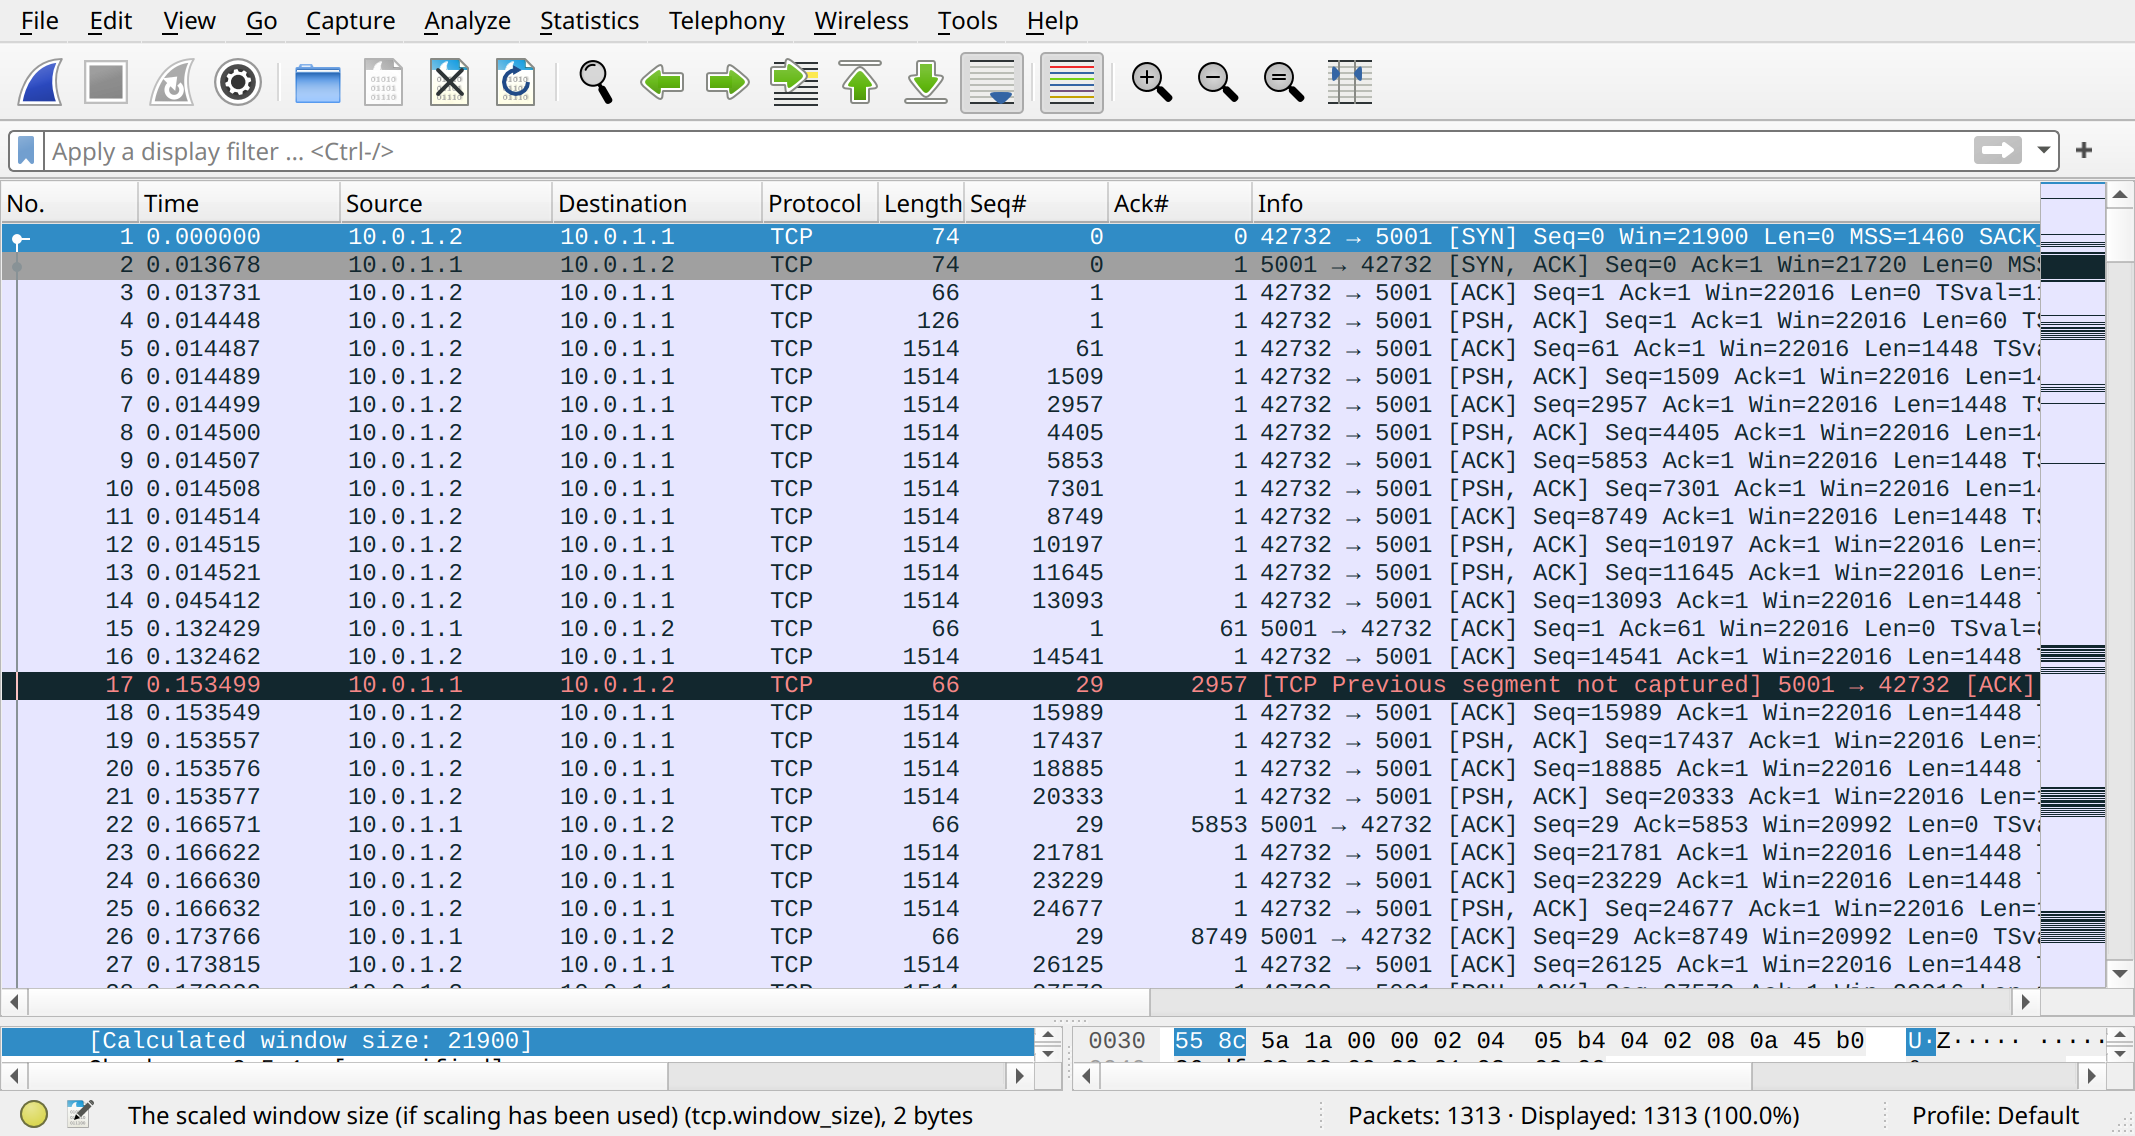
\includegraphics[width=\textwidth]{../reliable/wireshark-tcp-ex2-over}}%
\only<3->{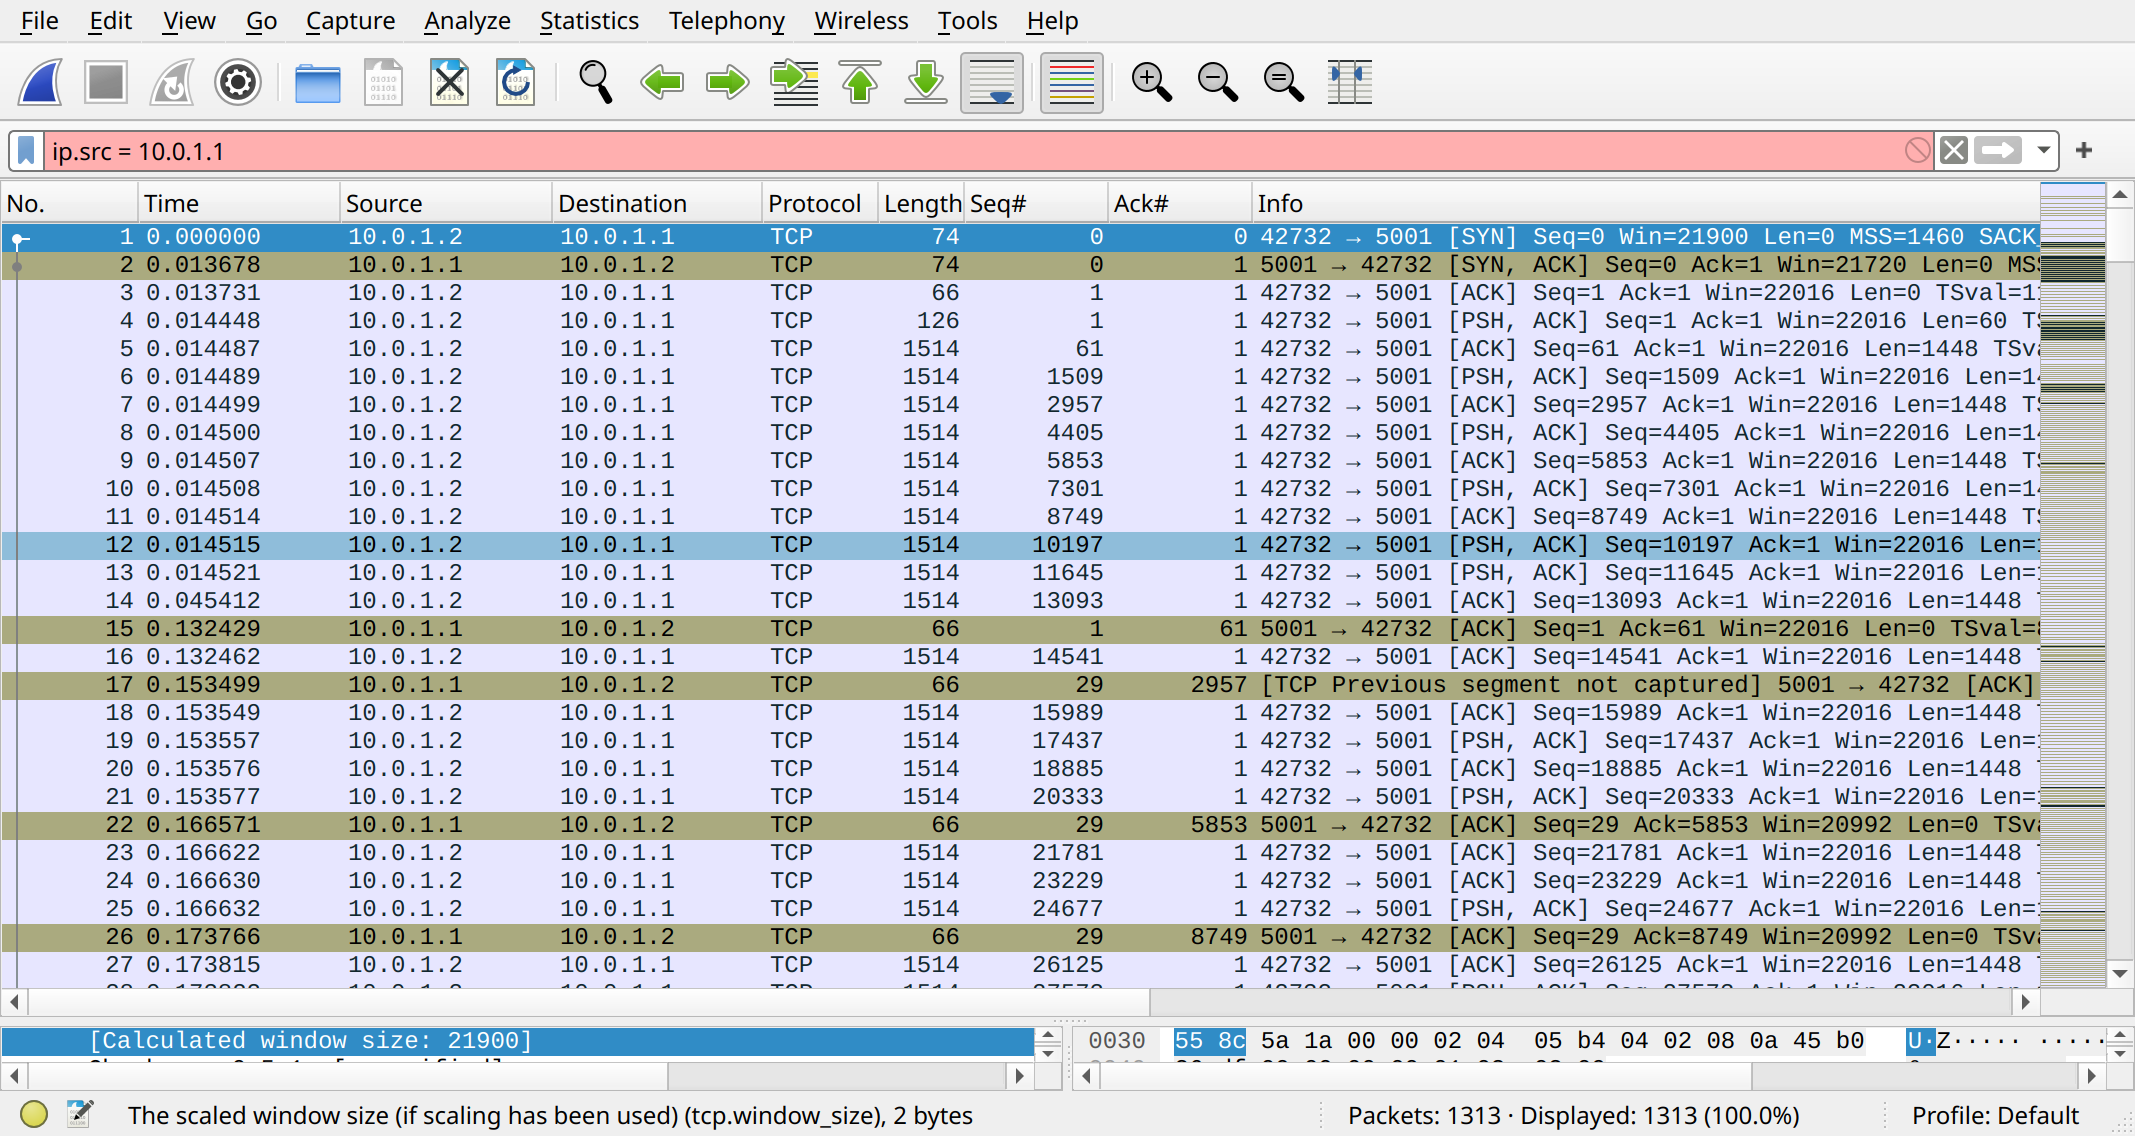
\includegraphics[width=\textwidth]{../reliable/wireshark-tcp-ex2-hi-dir}}%
};
\path (0, 0) rectangle (14.5, -7); % for bounding box
%\draw[overlay,help lines] (0, 0) grid (14, -8);
%\draw[overlay,help lines,dotted] (0, 0) grid[step=0.2] (14, -8);
\begin{visibleenv}<2-3>
\path[draw,red,very thick] (0, -1.5) rectangle (13.9, -2.125);
\node[red,overlay box,anchor=north,align=left] (c setup) at (6.95, -2.125) {
    connection setup, no data transferred 
};
\end{visibleenv}
\only<3>{\spy[rectangle,width=5cm,height=2.5cm,magnification=2] on (7.45, -1.7) in node at (12, 0);}
\begin{visibleenv}<3>
\node[overlay,overlay box,font=\small,anchor=east,align=left] at (9.5, -.5) {
    server+client sequence numbers \\
    advance by 1 to indicate where in setup
};
\end{visibleenv}
\begin{visibleenv}<4>
\path[draw,red,very thick] (0, -1.7) rectangle (13.9, -1.9);
\path[draw,red,very thick] (0, -4.2) rectangle (13.9, -4.39);
\path[draw,red,very thick] (0, -4.55) rectangle (13.9, -4.75);
\path[draw,red,very thick] (0, -5.5) rectangle (13.9, -5.75);
\path[draw,red,very thick] (0, -6.25) rectangle (13.9, -6.45);
\node[overlay box,align=left,anchor=north] at (6.95, -2.5) {
    connection is bidirectional \\
    from now, using olive color to show `backwards' packets
};
\end{visibleenv}
\only<5-6>{\spy on (7.25, -2.3) in node at (10, -1);}
\only<5-6>{\spy on (8, -4.3) in node at (12, -6);}
\begin{visibleenv}<5-6>
\path[draw,red,very thick] (6.55, -2.25 + .2) rectangle (7.5, -2.45 + .2);
    \node[overlay box,text=red,anchor=east,align=left] at (6.55, -2.35) {
        data packet with \\
        client bytes 1--60
    };
\path[draw,red,very thick] (7.55, -4.2) rectangle (8.5, -4.4);
    \node[overlay box,text=red,anchor=east,align=left] at (6.55, -4.3) {
        acknowledgement of \\
        client bytes up to 60
    };
\end{visibleenv}
\begin{visibleenv}<6>
\path[draw,red,very thick] (0, -2.25) rectangle (1.9, -2.45);
\path[draw,red,very thick] (0, -4.2) rectangle (1.9, -4.4);
\path[draw,red,dotted,double,ultra thick] (1, -2.45) -- (1, -4.2) node[midway,font=\small,fill=white,fill opacity=0.957,text=red,text opacity=1.0] {118 ms};
\end{visibleenv}
\begin{visibleenv}<7>
\path[draw,red,very thick] (12.6, -4.15) rectangle (13.3, -4.4);
\path[draw,red,very thick] (6.55, -4.2) rectangle (7.55, -4.4);
\path[draw,red,very thick] (6.55, -4.55) rectangle (7.55, -4.75);
\path[draw,red,very thick] (8.5, -4.55) rectangle (12, -4.75);
\only<7>{\spy[rectangle,width=10cm,magnification=1.5,height=1cm] on (10, -4.5) in node};
    \node[overlay box,text=red,anchor=south,align=left] at (6.55, -3.7) {
        jumps from server byte 0 to server byte 28 \\
        with no data sent \\
        wireshark IDs as missing packet
    };
% FIXME:  hilite len =0 and seq # 29
% FIXME: note missing data packet with bytes 1--28
% FIXME: screenshot scrolled down showing that
\end{visibleenv}
\end{tikzpicture}
\end{frame}

\begin{frame}[fragile]{a TCP connection}
\tikzset{
    overlay box/.style={fill=white,fill opacity=0.95},
}
\begin{tikzpicture}[
    spy using outlines={%
        rectangle,magnification=1.5,height=1cm,width=10cm,connect spies,%
        every spy on node/.append style={very thick},%
        ultra thick,%
    }
]
\node[overlay,anchor=north west,inner sep=0mm] (base) at (0, 0) {%
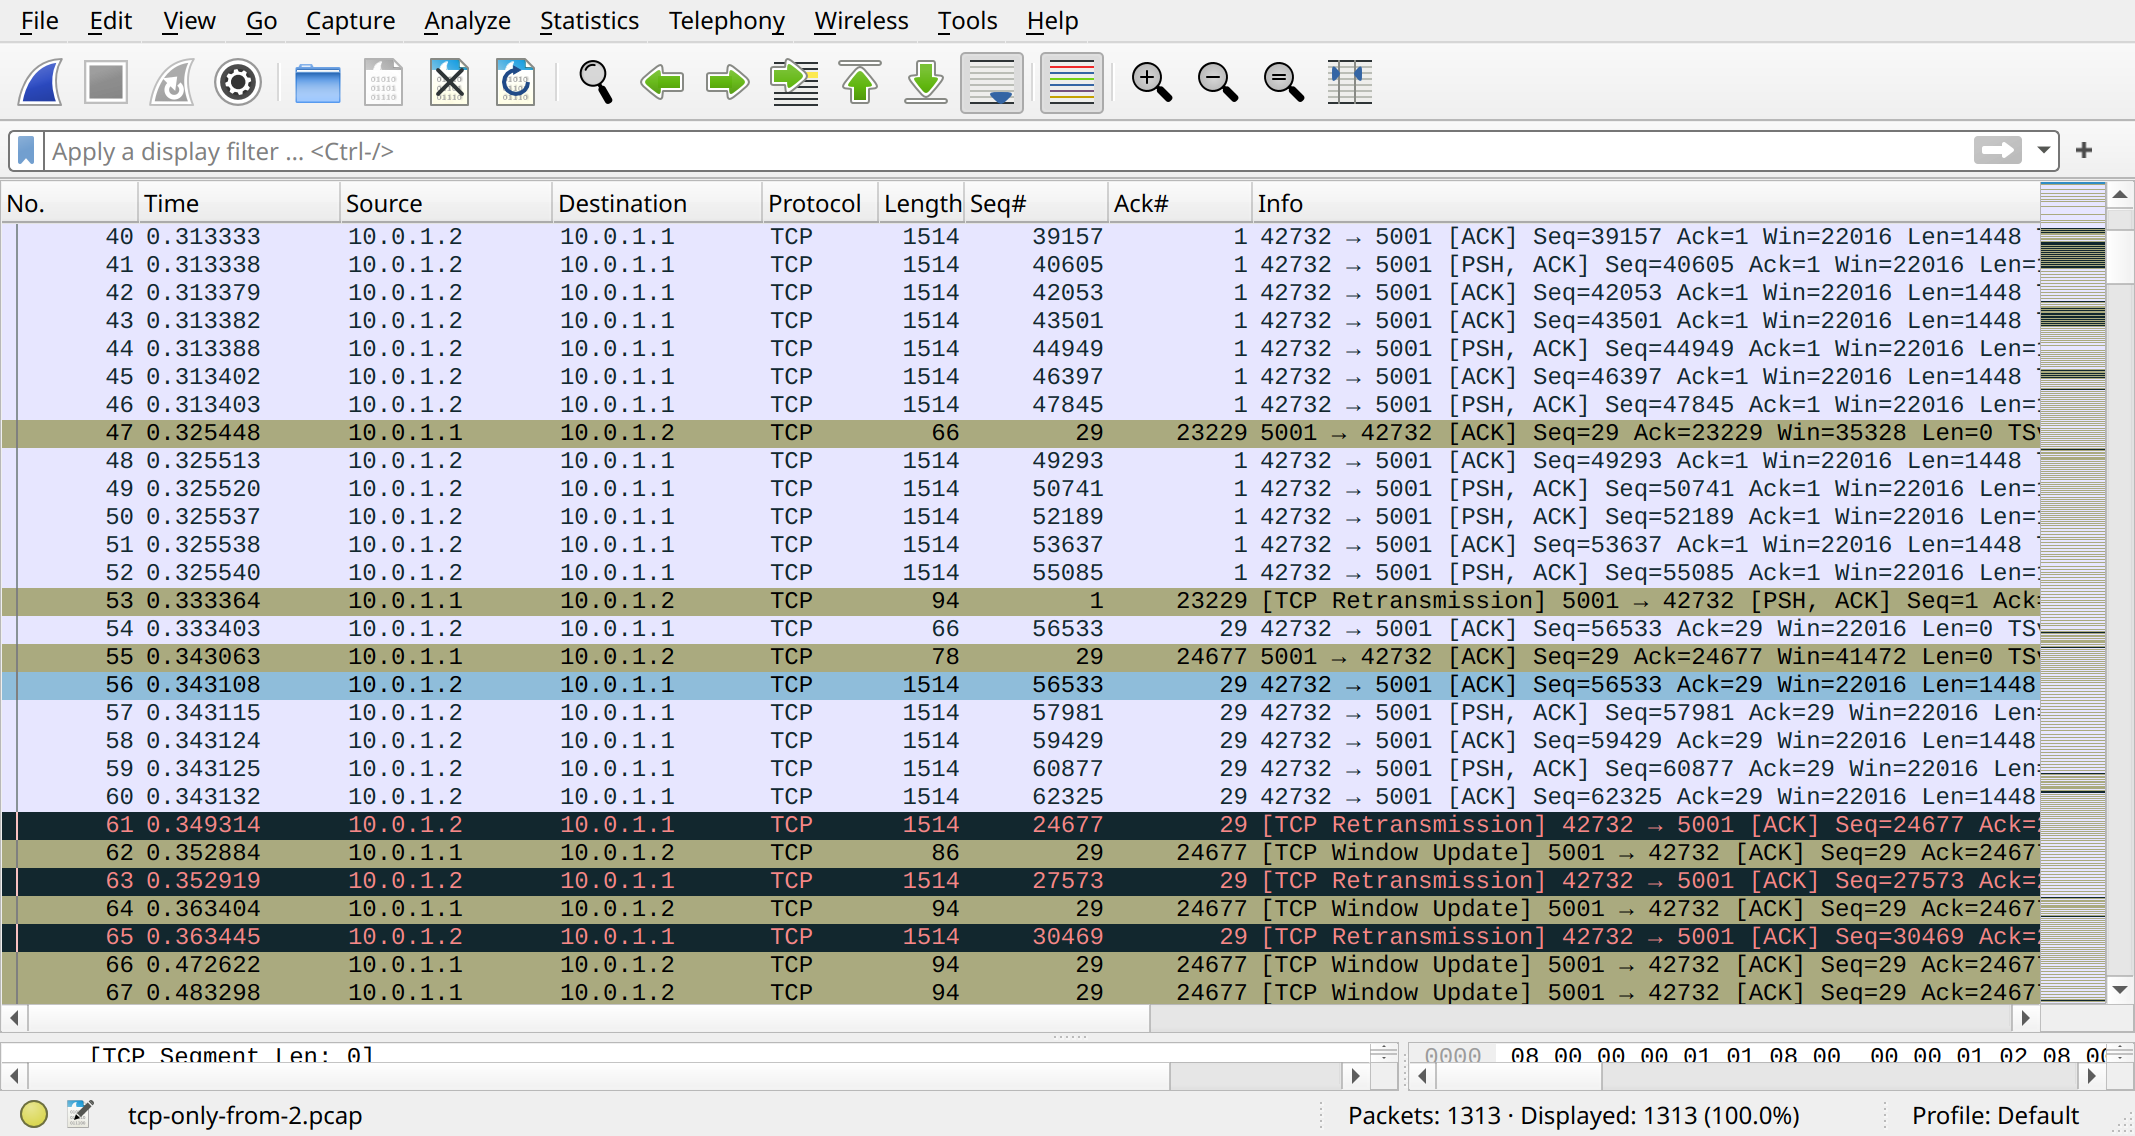
\includegraphics[width=\textwidth]{../reliable/wireshark-tcp-ex2-scrolled-server-retrans}%
};
\path (0, 0) rectangle (14.5, -7); % for bounding box
\spy on (10, -4.0) in node;
    \node[overlay box,text=red,anchor=south,align=left] at (6.55, -3.5) {
        scrolling down reveals retransmission later
    };
    \node[overlay box,text=black,font=\small,anchor=north,align=left] at (6.55, -4.5) {
        wireshark knows it's retransmission because \\
        sequence number sent by server went backwards
    };
\end{tikzpicture}
\end{frame}

\begin{frame}{first data packet}
\begin{tikzpicture}
\tikzset{
    overlay box/.style={fill=white,fill opacity=0.95},
}
\node[overlay,anchor=north west,inner sep=0mm] (base) at (0, 0) {%
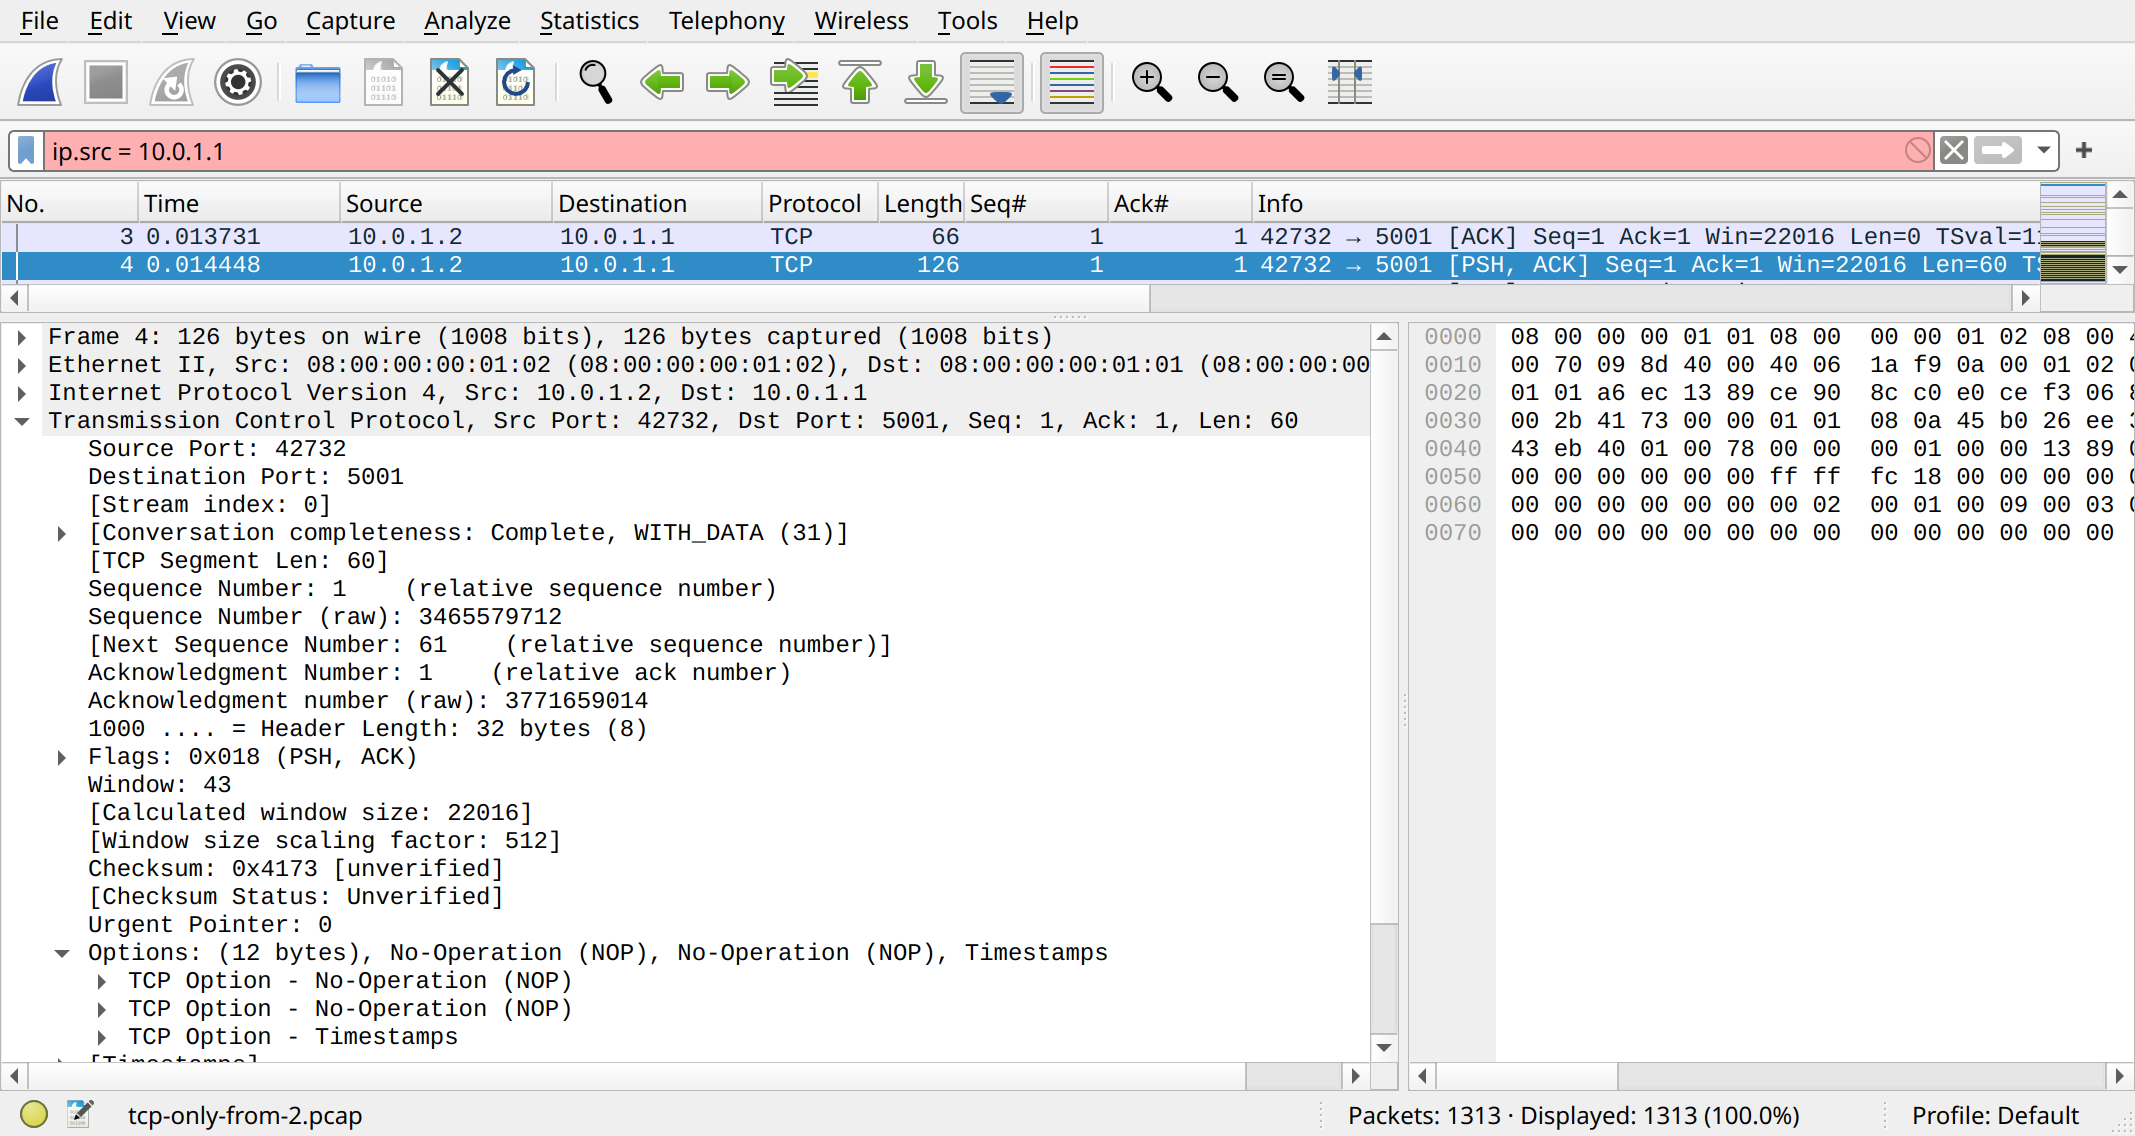
\includegraphics[%
    width=\textwidth,%
    % left bottom right top
    trim={0.5cm 2cm 20cm 10cm},clip,%
]{../reliable/wireshark-tcp-ex2-firstdata}%
};
\path (0, 0) rectangle (14.5, -7); % for bounding box
\draw[violet,overlay,help lines] (0, 0) grid (14, -8);
\draw[violet,overlay,help lines,dotted] (0, 0) grid[step=0.2] (14, -8);
%\spy[overlay,rectangle,magnification=1.7,height=7.5cm,width=10cm] on (3, -5) in node at (9, -3.5);
\begin{visibleenv}<2>
    \draw[red,very thick] (0.65, -2.45) rectangle (3.5, -2.75);
    \node[overlay box,text=red,anchor=west,align=left] at (3.5, -2.6) {
        not actually part of header \\
        computed using length from lower layer
    };
\end{visibleenv}
\begin{visibleenv}<3>
    \draw[red,very thick] (0.65, -2.75) rectangle (8.2, -3.25);
    \node[overlay box,text=red,anchor=north west,align=left] at (0.65, -3.25) {
        sequence numbers in header don't start at 0 \\
        wireshark converts to 0-based indices
    };
\end{visibleenv}
\begin{visibleenv}<4>
    \draw[red,very thick] (0.65, -2.75) rectangle (8.2, -3.55);
    \node[overlay box,text=red,anchor=north west,align=left] at (0.65, -3.55) {
        sequence number is \textit{first} byte being sent \\
        need to use segment length to know last byte's number \\
        (= what to ACK if receiving this)
    };
\end{visibleenv}
\begin{visibleenv}<5>
    \draw[red,very thick] (0.65, -3.55) rectangle (7.3, -4);
    \node[overlay box,text=red,anchor=north west,align=left] at (0.65, -4) {
        ack number indicates received start-of-connection stuff \\
        and nothing else (in case server sent something)
    };
\end{visibleenv}
\begin{visibleenv}<6>
    \draw[red,very thick] (0.65, -4.3) rectangle (3.85, -4.6);
    \node[overlay box,text=red,anchor=north west,align=left] at (0.65, -4.6) {
        PSH = no more data right now \\
        ACK = acknowledgment number is valid 
    };
\end{visibleenv}
\begin{visibleenv}<7>
    \draw[red,very thick] (0.65, -4.55) rectangle (5.15, -5.35);
    \node[overlay box,text=red,anchor=south west,align=left] at (0.7, -4.5) {
        window scaling option in use \\
        (scaling factor only sent in connection setup)
    };
\end{visibleenv}
\begin{visibleenv}<8>
    \draw[red,very thick] (0.65, -6.1) rectangle (10.3, -7.2);
    \node[overlay box,text=red,anchor=south west,align=left] at (0.7, -6.0) {
        no-operation options used to make TCP header size multiple of 4
    };
\end{visibleenv}
\end{tikzpicture}
\end{frame}

\begin{frame}{sequence numbers graph}
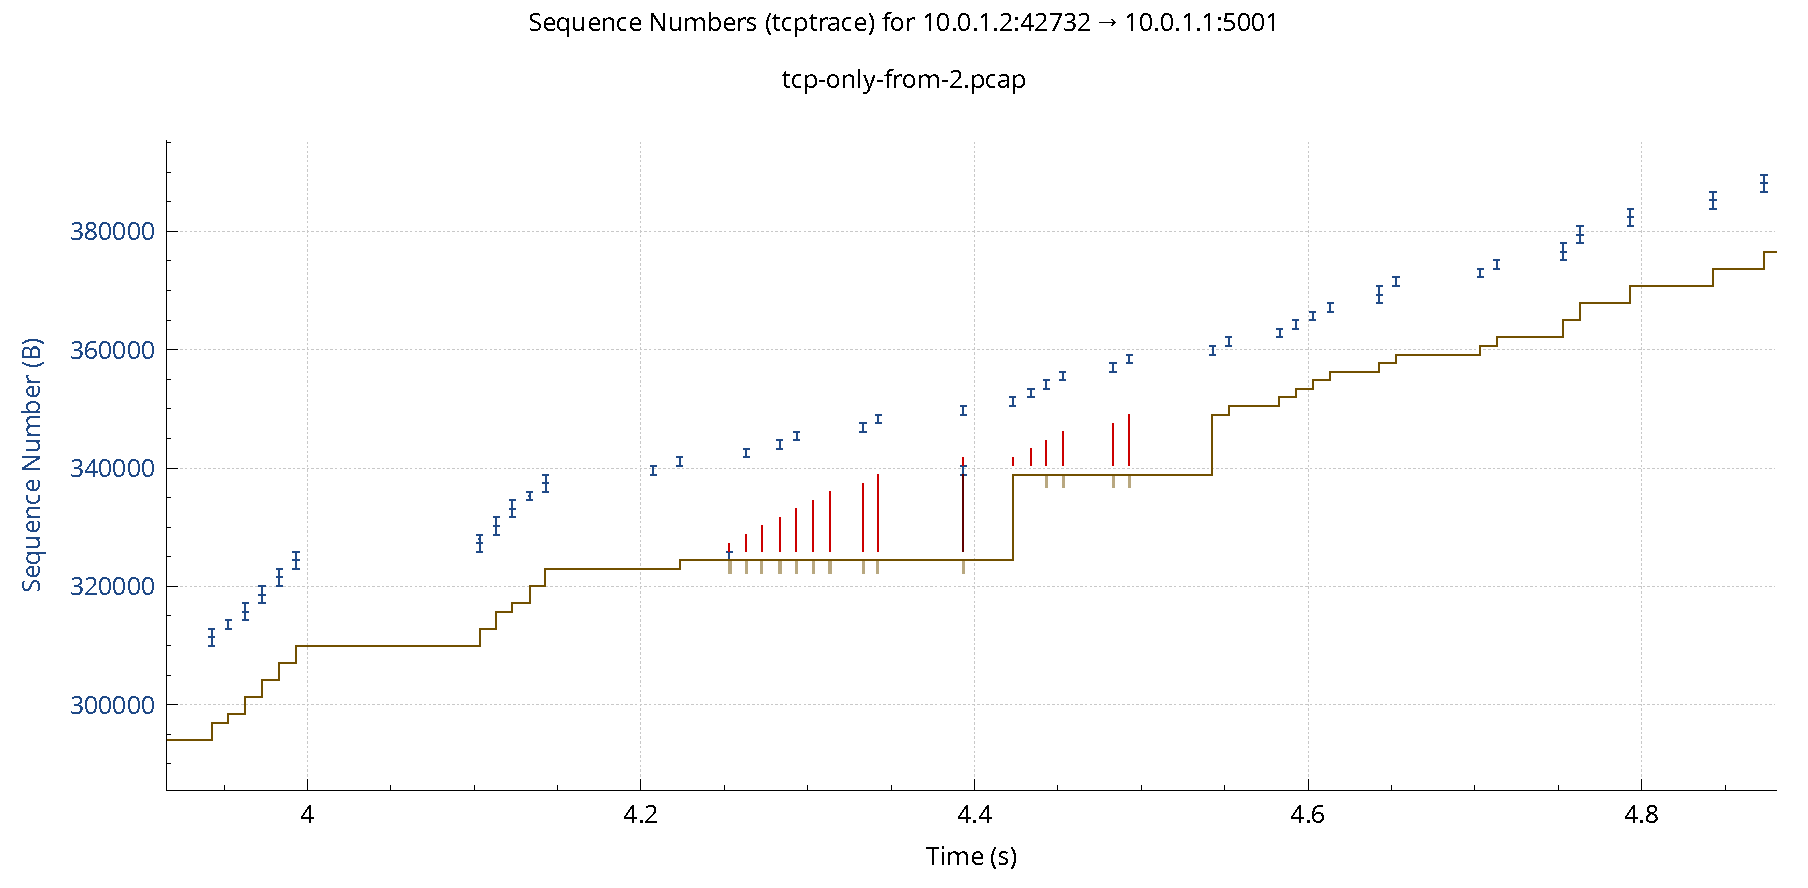
\includegraphics[width=\textwidth]{../reliable/tcptrace-example2}
% FIXME: line at bottom = acknowledgment number from server
% FIXME: blue "I"s = data packets sent
% FIXME: notches on acknowledgment line = duplicate acknowledgments
% FIXME: red lines = selective acknowledgment info
% FIXME: note --- sending new packets triggered by ACK
    % and this is observed from the client
    % so each blue line matches a red line
% FIXME: note slowdown due to congestion
\end{frame}

\begin{frame}{reading thigs graph}
    \begin{itemize}
    \item bottom line = last ack number
    \item notches on bottom line = duplicate acks
    \item red lines = selective ACK info
    \end{itemize}
\end{frame}

\begin{frame}{diff. timing in opposite direction}
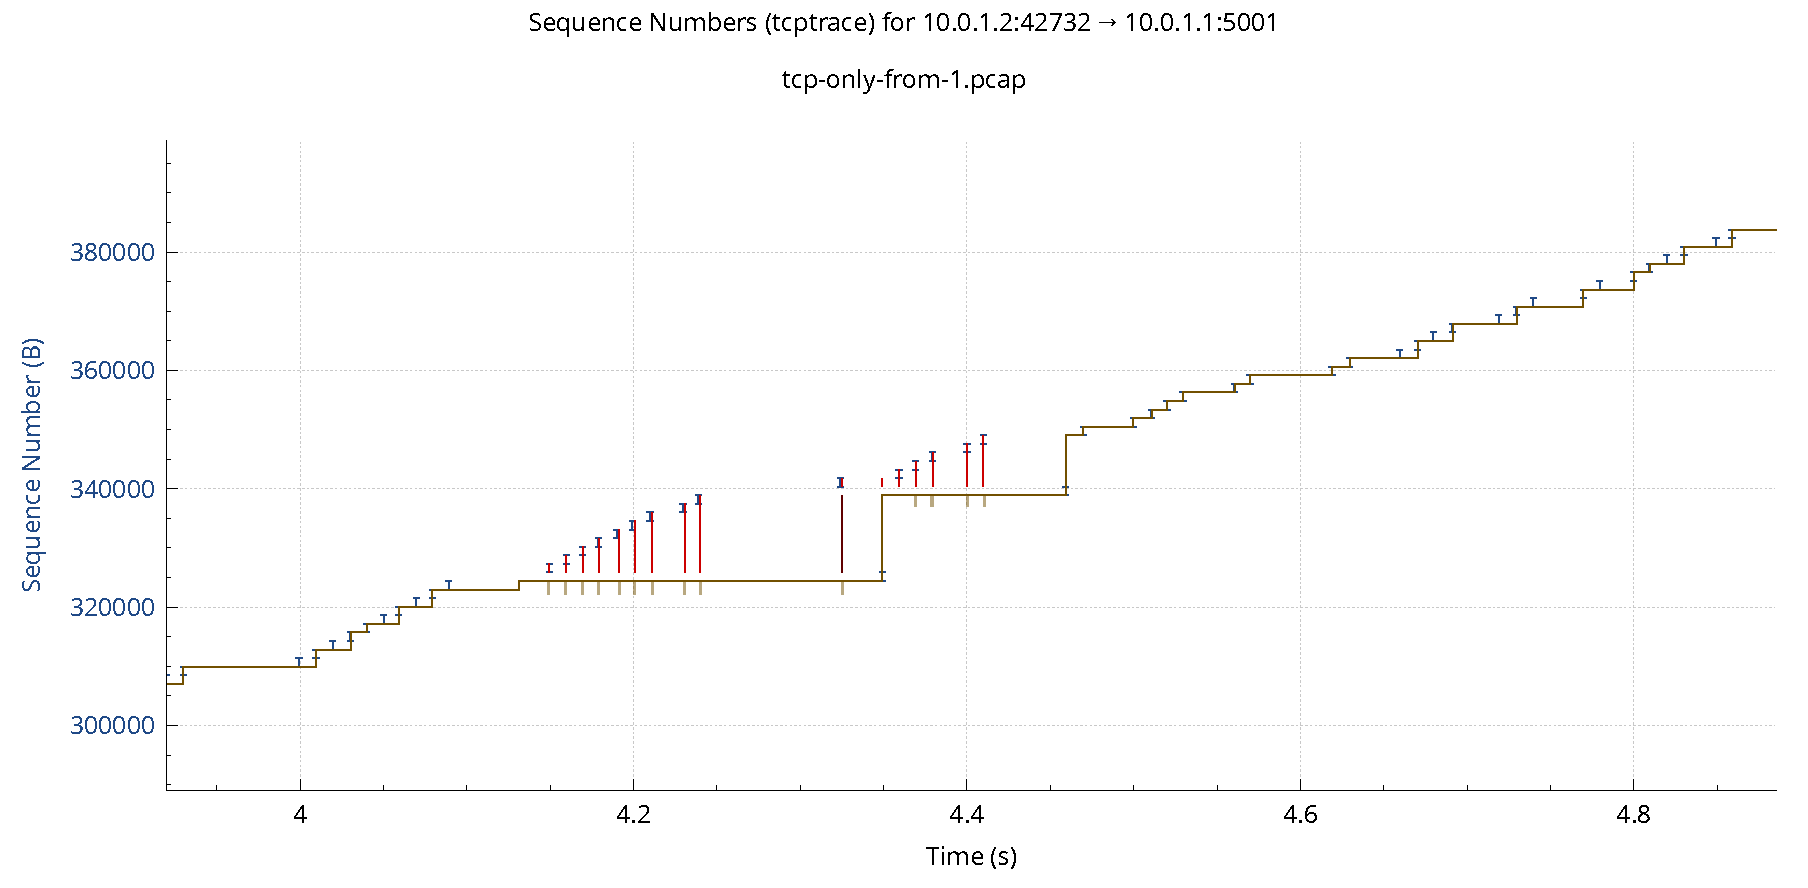
\includegraphics[width=\textwidth]{../reliable/tcptrace-example2-oppdir}
% FIXME: note different timing
\end{frame}


% FIXME: example of TCP in practice
    % FIXME: show packet trace mostly through wireshark screenshots
        % interleave with TCP format diagram from standard
    % mention I was doing large SSH transfer
    % look at client -> server packet from that transmission
    % note existence of Ethernet, IPv4 parts
    % look at TCP part
        % talk about flags
        % talk about sequence number, acknowledgment number
        % show window size, talk about calculation in packet format
        % show timestamp option

    % look at duplicate ACK -- wireshark search
        % show increasing SACK window

    % find retransmissions
        % look for trace with real retransmissions?

    % FIXME: get trace which is bandwidth limited --- from VM?

    % add ack/seq column, show

    % show ACK-only packet

% FIXME: show graphs
    % sequence number
        % include tight zoom to show sending window pattern
    % round-trip time

% FIXME: preview: congestion


\section{backup slides}
\begin{frame}{backup slides}
\end{frame}

\end{document}
